\documentclass{article}

\usepackage[utf8]{inputenc} % on touche pas 
\usepackage{graphicx}
\usepackage[bottom = 2 cm]{geometry}
\usepackage[french, english]{babel}
\usepackage{amsmath}
\usepackage{amsfonts}
\usepackage{amssymb}
\usepackage{numprint}
\usepackage{hyperref}
\usepackage[T1]{fontenc}
\usepackage{titling}
\usepackage[nottoc, numbib]{tocbibind}
\usepackage[dvipsnames]{xcolor}
\usepackage{fancyhdr}
\usepackage{blindtext}
\usepackage{titlesec}
\usepackage{titletoc}
\usepackage{array}
\usepackage{listings}
\usepackage{subfig}
\usepackage{float}
%\usepackage[amssymb]{SIunits}

\usepackage[style = numeric]{biblatex}
% \bibliographystyle{unsrt}
% \addbibresource{biblio.bib}
\bibliography{biblio.bib}


% \setlength{\hoffset}{-18pt}
% \setlength{\oddsidemargin}{0pt} % Marge gauche sur pages impaires
% \setlength{\evensidemargin}{9pt} % Marge gauche sur pages paires
% \setlength{\marginparwidth}{54pt} % Largeur de note dans la marge
% \setlength{\textwidth}{481pt} % Largeur de la zone de texte (17cm)
% \setlength{\voffset}{-18pt} % Bon pour DOS
\setlength{\marginparsep}{7pt} % Séparation de la marge
% \setlength{\topmargin}{0pt} % Pas de marge en haut
\setlength{\headheight}{20pt} % Haut de page
% \setlength{\headsep}{10pt} % Entre le haut de page et le texte
\setlength{\footskip}{50pt} % Bas de page + séparation
\setlength{\textheight}{21cm} % Hauteur de la zone de texte (25cm)
\setlength{\parskip}{1em}
\setlength{\parindent}{1em}

\setlength\tabcolsep{8pt}
\renewcommand{\arraystretch}{1.4}

\pagestyle{fancy}
\fancyhf{}
\rhead{École des Mines de Paris}
\lhead{MIG L'Eau après la Mine}
\rfoot{\vspace{-0.7 cm}\thepage}


%style de sections
\titleformat{\section}
    {\Large\bfseries}
    {\thesection}
    {1 em}
    {}
\titleformat{\subsection}
    {\large\bfseries}
    {\qquad\thesubsection}
    {1 em}
    {}
\titleformat{\subsubsection}
    {\large\bfseries}
    {\qquad\qquad\thesubsubsection}
    {1 em}
    {}

\renewcommand{\thesection}{\Roman{section})} % je préfére les parenthèses 
\renewcommand{\thesubsection}{\arabic{subsection})} % c'est + joli
\renewcommand{\thesubsubsection}{\alph{subsubsection})} 
% sinon on peut mettre Partie 1 ... aussi 

%paramétrage de la table des matières
% \titlecontents{section}
%             [0pt]
%             {\bfshape}%
%             {\contentsmargin{0pt}%
%             \bfseries
%             \makebox[0pt][r]{\large\thecontentslabel\enspace}%
%             \large}
%             {\contentsmargin{0pt}\large}
%             {\hfill\textbf{\contentspage}}
%             [\addvspace{1pc}]
            
\dottedcontents{section}[]{\Large\bfseries}{2 em}{0.6 em}
% \titlecontents{subsection}
%             [20 pt]
%             {}%
%             {\contentsmargin{0pt}\bfseries            \makebox[0pt][r]{\large\thecontentslabel\enspace}%
%             \large}
%             {\contentsmargin{0pt}\large}
%             {\hfill\textbf{\contentspage}}
%             [\addvspace{1pc}]
\dottedcontents{subsection}[30 pt]{\large\bfseries}{2 em}{0.6 em}    
% \titlecontents{subsubsection}
%             [40 pt]
%             {}
%             {\contentsmargin{0pt}\bfseries\makebox[0pt][r]{\large\thecontentslabel\enspace}\large}
%             {\contentsmargin{0pt}\large}
%             {\hfill\textbf{\contentspage}}
%             [\addvspace{1pc}]
\dottedcontents{subsubsection}[60 pt]{\bfseries}{2 em}{0.6 em}    

\makeatletter
\renewcommand\listoffigures{%
    \section{\listfigurename}% Used to be \section*{\listfigurename}
      \@mkboth{\MakeUppercase\listfigurename}%
              {\MakeUppercase\listfigurename}%
    \@starttoc{lof}%
    }
\makeatother

\lstset{numbers=left, 
    stepnumber=5, 
    firstnumber=1, 
    breaklines = true,backgroundcolor=\color{lightgray!20!},
    rulecolor=\color{black},
    frame=tb
    }%, numbersep=5pt}
    
    
\lstdefinelanguage{hytec}{language = Python,
    alsoletter =/,
    alsoletter =-,
    classoffset = 0,
    morekeywords = {darcy,velocity,diffusion-coeff,condition,coordinates,coeff,database,solver-regime,grid-regime,flow-regime,zone,head,porosity,permeability,geochem,boundary,exclude, unit,extend,kinetics,exclude,using,mineral,define,duration,timestep},
    keywordstyle={\color{blue}},
    classoffset = 1,
    % otherkeywords = {0,1,2,3,4,5,6,7,8,9,-,.},
    morekeywords = [2]{0,1,2,3,4,5,6,7,8,9,-,.},
    keywordstyle=[2]{\color{orange}},
    classoffset = 2,
    otherkeywords = {chimie_granite,chimie_granite_frac,chimie_residus_boues,chimie_residus_sable},
    morekeywords = [3]{chimie_granite,chimie_granite_frac,chimie_residus_boues,chimie_residus_sable,chimie_steriles,flux, top,gases, minerals,left,right,top},
    keywordstyle = [3]{\color{red}},
    classoffset = 4,
    morekeywords = [4]{tot, pH, fug,surface,power,rate,area,species,basis, variable,start,maximum,courant,factor,composition,logK,mg/l,umol/l,mmol/l,m/s,y-term,w-term},
    keywordstyle = [4]{\color{ForestGreen}}
}



\definecolor{dkgreen}{rgb}{0,0.6,0}
\lstdefinelanguage{gmsh}{
%   basicstyle=\footnotesize\ttfamily\color{black},   
  breakatwhitespace=false,
  breaklines=true,               
  captionpos=t,                   
  commentstyle=\color{dkgreen},
  deletekeywords={...},          
  escapeinside={\%*}{*)},                  
  frame=tb, %top/bottom lines
  language=C++,                
  keywordstyle=\color{purple},  
  morekeywords={Point, Line, Surface, Ellipse, Volume, Physical, Circle, Line Loop, Plane, Loop, newp, newreg, newl, news, newll, newv, Mesh, CharacteristicLengthMax, CharacteristicLengthMin, SetFactory, Spline, BSpline, Rectangle, Disk, Torus, Wedge, Cone, Block, Sphere, Cylinder,
    BooleanIntersection, BooleanDifference, BooleanFragments, BooleanUnion,
    Delete, Rotate, Extrude, Pi, StrCat,
  DefineConstant, ReadOnly, Step, Min, Max, Name, AutoCheck, Visible, Choices},  
  identifierstyle=\color{black},
  stringstyle=\color{blue}, 
%   numbers=left,                 
%   numbersep=5pt,                  
%   numberstyle=\tiny\color{black}, 
  rulecolor=\color{black},        
  showspaces=false,               
  showstringspaces=false,        
  showtabs=false,                
%   stepnumber=1,                   
  tabsize=5,                     
  title=\lstname,                 
}






\definecolor{couleurmines}{RGB}{22, 91, 160}

\title{ \textbf{ {\color{couleurmines}
\Huge{\textsc{École des Mines de Paris}}\\
\vspace{1.5 cm}
MIG L'Eau après la Mine\\\vspace{1 cm}Synthèse du projet}}
\vspace{1 cm}
}

\author{%Projet réalisé par les élèves : \\ 
Sophian \textsc{Akkari},
Tom \textsc{Boezennec}, 
Paul \textsc{Colombel}, 
Florestan \textsc{Fontaine},\\
Yiqiong \textsc{Hu}, 
Tasnime \textsc{Ouchtar}, 
Guillaume \textsc{Ramos}, 
Louison \textsc{Rapin}, 
Guillaume \textsc{Rouy},\\ 
Louis-Justin \textsc{Tallot}, 
Gabrielle \textsc{Vernet}, 
Guillaume \textsc{Vigne}, 
Robin \textsc{Willocquet}\\
%\\ qui furent encadrés par les enseignants-chercheurs  : \\
\\ encadrés par les enseignants-chercheurs \\
Irina \textsc{Sin}, 
Sophie \textsc{Guillon}, 
Nicolas \textsc{Seigneur}
et Vincent \textsc{Lagneau} \\
du Centre de Géosciences (Mines ParisTech - PSL)}

\date{\vspace{2 cm}Novembre - Décembre 2020}



\begin{document} % début du document %%%%%%%%%%%%%%%%%%%%%%%%%%%%%%%%%%%%%%%%%%%%%%%%%%%%%%%%%%%%%%%%%
\selectlanguage{french}

\maketitle
\thispagestyle{empty}
\vspace{2 cm}
\begin{center}
    
\includegraphics[width = 0.4\linewidth]{logoMPT.png}
\end{center}
\newpage
\pagenumbering{gobble}

\section*{Remerciements}
Les élèves remercient sincèrement les différents intervenants : 
\begin{itemize}
    \item Camille \textsc{Chautard} (Orano Mining)
    \item Caroline \textsc{Benesteau} (Orano Mining)
    \item Nadine \textsc{Himeur} (Orano Mining)
    \item Michael \textsc{Descostes} (Orano Mining)
    \item Joachim \textsc{Schick} (Orano Mining)
    \item Guillaume \textsc{Kern} (Orano Mining)
    \item Louis \textsc{Raimbault} (Mines ParisTech - PSL, Centre de géosciences) 
    \item  Emmanuel \textsc{Ledoux} (Mines ParisTech - PSL)
    \item Valentin \textsc{Robin} (Université de Limoges, Laboratoire E$^2$LIM) 
    \item Jean-Luc \textsc{Viallesseche} (Eaux de Limoges Métropole)
    \item Pascale \textsc{Blanchard} (IRSN)  
    \item Isabelle \textsc{Dublineau} (IRSN)    
    \item  Pascale \textsc{Nalon} (Mines ParisTech - PSL, bibliothèque de Fontainebleau)
    \item Anne \textsc{Schmid} (Mines ParisTech - PSL, bibliothèque de Fontainebleau)
    \item Roland \textsc{Desbordes (CRIIRAD)}
\end{itemize}

ainsi que leurs encadrants :

\begin{itemize}
    \item Irina \textsc{Sin} (Mines ParisTech - PSL, Centre de géosciences) 
    \item Sophie \textsc{Guillon} (Mines ParisTech - PSL, Centre de géosciences) 
    \item Nicolas \textsc{Seigneur} (Mines ParisTech - PSL, Centre de géosciences) 
    \item Vincent \textsc{Lagneau} (Mines ParisTech - PSL, Centre de géosciences) 
\end{itemize}


\vspace{0.5 em}
\begin{center}

\includegraphics[height = 40pt]{oranologo.png}
\hspace{0.3em}

\includegraphics[height = 40pt ]{logoMPT.png}
\hspace{0.3em}

\includegraphics[height = 40pt ]{logoUNILIM.png}
\hspace{0.3em}

\includegraphics[height = 40pt ]{Logo-PEIRENE.png}

\vspace{0.2 em}

\includegraphics[height = 80pt ]{logoeaulimoges.png}
\hspace{0.3em}

\includegraphics[height = 40pt ]{logoIRSN.png} 
\hspace{0.3em}

\includegraphics[height = 40pt]{logo_ASN.png}
\hspace{0.3em}

\includegraphics[height = 40pt]{logo_BRGM.png}

\end{center}
%Est-ce vraiment utile de mettre tous les logos ? On cite déjà les différentes entreprises/universités/labos... --S qui est S le sang
% oui c'est joli et il reste de la place sur la page et je me suis embêté à les mettre

\newpage
\pagenumbering{gobble}
\lfoot{
\includegraphics[width = 3 cm]{logoMPT.png}}
\tableofcontents

\newpage

\begin{abstract}
% A revoir
La France, autrefois grand pays minier, possède aujourd’hui de nombreux sites miniers ayant cessé toute activité, et devant donc être réhabilités : c'est ce qu'on appelle l'\emph{après-mine}

L’après-mine comprend ainsi des enjeux sanitaires et environnementaux (comme la gestion des déchets), sociaux (notamment l'entente avec les associations et les habitants), politiques (par exemple le respect des normes) et économiques.

La présente étude concerne la majorité de ces aspects. Elle a pour but d'identifier les différents acteurs de l'après-mine et ses problématiques, tout en essayant d’y répondre. Elle aborde la question des normes à respecter, le respect de l’environnement et des sociétés locales mais aussi des aspects plus techniques comme la gestion des polluants.

Nous étudions plus particulièrement le cas des anciennes mines d'uranium, ainsi que le traitement de l’eau et du radon. Une attention spécifique est portée à la nécessité du traitement de l’eau pour l’ancienne mine d’uranium de la Ribière.

Nous proposons ainsi une synthèse des problématiques de l’après-mine comprenant les contraintes des différentes normes, les restrictions imposées par les acteurs sociaux, une comparaison des différents types de traitement existants et la gestion de l'après-mine par les principaux pays miniers. Les principaux polluants, comme le radon, l'uranium et le radium, peuvent être traités efficacement. Un modèle hydrogéochimique établi pour notre étude permet également de conclure sur le cas de la Ribière : aucun traitement ne semble nécessaire pour l’uranium.

L’après-mine est ainsi un problème très important pris au sérieux et bien résolu par les exploitants mais souvent méconnu des populations. Bien que de nombreuses solutions soient mises en place, il est nécessaire de faire de l’information et de donner à l’après-mine une importance plus grande encore que celle qui lui est accordée aujourd’hui.
\end{abstract}

{\selectlanguage{english}
\begin{abstract}
France used to be a major mining country. Yet, the exploitation of most of French mines has been completely interrupted and the mining sites need to be rehabilitated. This rehabilitation is the post-mine process. It aims at addressing health related and environmental issues (such as the gestion of mining waste), as well as social (such as finding consensus with local associations and populations), political (for instance the accordance with standards) and economical issues.

This study deals with most of these questions. Its goal is to identify both the different parties the post-mine process involves and the issues it brings up, to try to solve them. It also deals with technical aspects of the process such as the treatment of polluted mining waste. We will focus on the former uranium mines, on the treatment of water and on the alleviation of radon. We will particularly study the necessity of water treatment in the former uranium mine La Ribière. After having synthesized these questions, we will draw a comparison of the diverse existing means of water treatment and investigate the strategies implemented by the major mining countries to deal with the post-mines problematics. 

We will acknowledge that the major polluting substances (radon, radium, uranium…) can be efficiently treated. A hydrogeochemical modelisation of the La Ribière site will enable us to determine whether if the treatment of the effluents is necessary. The post-mine process is a serious issue which is often well dealt with by the exploiting firms but quite ignored by the local populations. Although many measures have been enforced, it is still necessary to inform the inhabitants of former mining areas to make bring the post-mine process into even wider attention. 
\end{abstract}
}

\newpage
\pagenumbering{arabic}
\section*{Introduction}
\addcontentsline{toc}{section}{Introduction}

\newpage
\section{Contexte de l’après-mine} %bonjour irina :)

\subsection{Histoire minière de la France}

\paragraph{} Lorsqu’on parle de mine, on a souvent en tête l’image du mineur de charbon portant casque avec lampe frontale ainsi que bleu de travail, noirci par son travail et éreinté de ses journées, qui descend chaque jour dans le ventre de la mine pour excaver la roche et nourrir sa famille. L’histoire minière française est bien plus diverse que cela en réalité : bien que le charbon occupe une place importante, surtout dans le Nord de la France, bien d’autres métaux ont été exploités en France - dont notamment l’uranium.

La décision d’exploiter un gisement est le résultat d’un processus appelé exploration. Il vise à établir, avec le plus haut niveau de confiance possible, la géologie du site. On effectue pour cela des sondages puis des forages et des analyses géochimiques. Si le filon est trouvé et que l’on ne sait rien de plus, on parle de ressource. Dès lors que l’on est assuré que l’exploitation est possible, on parle de réserve. Pour décider de l’exploitation, il faut réunir plusieurs conditions : une ressource en quantité suffisante, des techniques d’exploitation suffisamment adaptées et des risques financiers limités. Une fois l’exploitation décidée, vient la phase de développement. Cette dernière consiste à décider des techniques d’exploitation et à étudier les impacts sociaux et environnementaux afin d’obtenir les autorisations légales. Il se passe ainsi une dizaine d’années entre les premières études géologiques et le début de l’exploitation. 

La moitié des mines dans le monde sont à ciel ouvert, mais ces dernières représentent 90 \% de la quantité extraite en masse. La plupart des mines existantes à ciel ouvert sont excavées par motif en escalier : cela permet de voir les différentes strates et différentes époques d’exploitation \cite{raimbault_mine_2020}.

La France est un pays avec un passif minier bien présent et ancré dans les esprits. En effet, c’est vers l’ère industrielle qu’apparaissent de nombreuses mines qui mèneront à divers bassins miniers français : or, cuivre, fer, étain, manganèse, tungstène, bauxite…. Vers le début du XXème siècle, on compte environ 800 sites miniers en France. L’industrie minière est régulée par divers organismes car les conséquences de l’exploitation touchent de nombreux acteurs \cite{ledoux_notions_2020}.

L’uranium, élément 92 du tableau périodique, est le centre de notre attention ici. En effet, il est au fondement de l’énergie nucléaire massivement utilisée en France et sert d’élément principal pour l’arme nucléaire. On en trouve naturellement, principalement de l’isotope 238. Et pourtant, c’est surtout l’isotope 235 qui intéresse le monde scientifique : en effet, son activité radioactive est plus élevée, bien qu'il représente 0,7 \% de l’uranium mondial. L'uranium comporte 2 degrés d’oxydation : le +IV se trouve surtout sous terre, il est insoluble et réducteur et est celui qui est prévalent (avec comme exemples de minerais porteurs d'uranium l'uraninite, ou la coffinite) ; le +VI se trouve principalement en surface, et est soluble et oxydant (avec comme exemple de minerai l'autunite). On le trouve aussi en quantité moindre en rétention dans de l’argile ou des oxydes \cite{descostes_introduction_2020}.

Les gisements d’uranium ont des concentrations très diverses, comme le montre la figure \ref{fig:gisements_uranium}. La plupart des gisements ont une concentration en uranium de l’ordre de 0,1 \% mais elle peut atteindre jusqu’à 10 \% dans certaines mines canadiennes (Cigar Lake, McArthur River) \cite{raimbault_mine_2020}.


\begin{figure}[H]
    \centering
    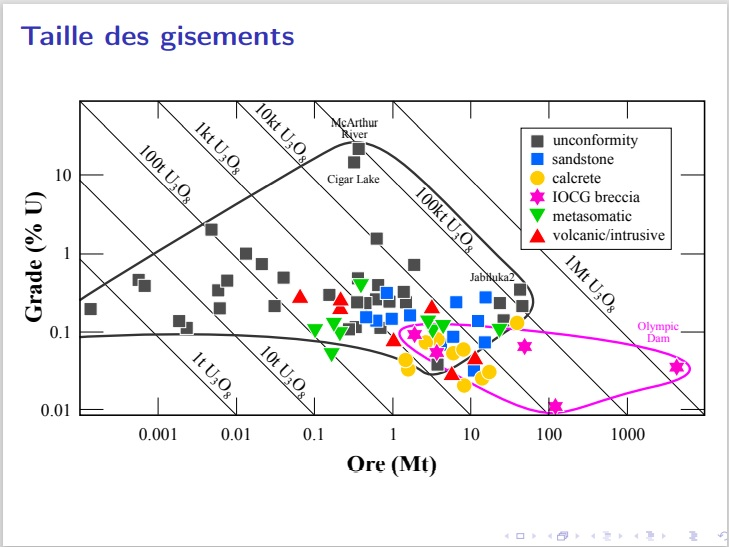
\includegraphics[width = \linewidth]{I_A_1.jpg}
    \caption{Taille des gisements d'uranium selon leur teneur et la quantité de minerai \cite{raimbault_mine_2020}}
    \label{fig:gisements_uranium}
\end{figure}
%Image 1 (prez L. Raimbault)

En France, la volonté d’exploiter l’uranium date de la fin de la Seconde Guerre mondiale. Il s’agit alors d’un enjeu stratégique majeur puisque l’objectif était d’assurer l’approvisionnement en uranium de l’armée, qui en avait besoin pour développer l’arme nucléaire. La première mine d’uranium française a ainsi ouvert en 1948. Avec la décision de développer le nucléaire civil, il a ensuite fallu approvisionner en combustibles les centrales nucléaires pour assurer l’indépendance énergétique du pays. L’épuisement des gisements français et la découverte de gisements bien plus importants à l’étranger, notamment au Niger, entraînent la fermeture des mines françaises. La dernière mine d’uranium ferme ainsi en 2001. Au total, il y a près de 230 sites miniers liés à l’uranium en France, qui ont produit environ 76 000 t en un demi-siècle (une mine française produisait quelques tonnes d’uranium par an). Ces sites sont situés dans le Massif Central ainsi qu’en Bretagne et en Vendée (voir la carte en figure \ref{fig:sites_orano}). Le Limousin est à lui seul à l’origine de près de la moitié de la production française \cite{descostes_introduction_2020}.

%    Image 2 (prez Orano C. Benesteau)
\begin{figure}[H]
    \centering
    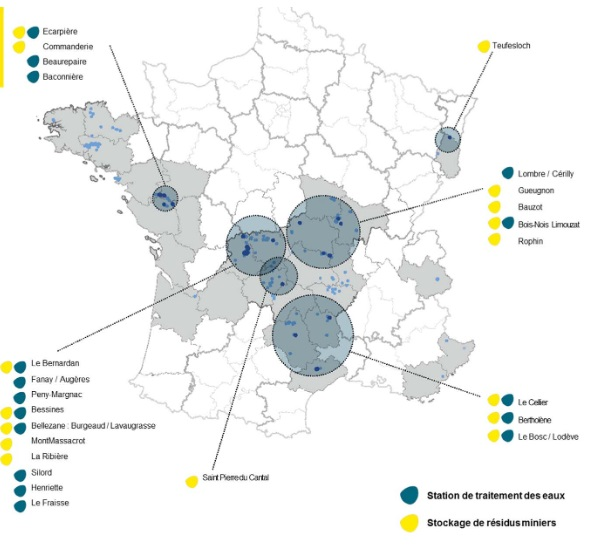
\includegraphics[width=\linewidth]{I_A_2.jpg}
    \caption{Carte des sites miniers uranifères en France (Orano)}
    \label{fig:sites_orano}
\end{figure}

Les mines sont régies par différentes autorités : le code minier par exemple, qui pose un cadre juridique récent, ainsi que diverses polices des mines, dont la police des ICPE (installation classée pour la protection de l’environnement), créée en 1976. Des polices liées à des domaines transverses tels que l’eau, les déchets, ou encore la santé, interviennent elles aussi sur ce sujet qui lie ainsi de nombreux domaines. Le RGIE (\emph{Règlement Général des Industries Extractives}) complète enfin ces polices des mines. [IRSN]

Ces polices sont nécessaires car les risques miniers sont importants et peuvent causer de lourds dégâts. On parle d’instabilité mécanique pour désigner les risques d’effondrement ou d’affaissement de pans de mines, ou de rupture des digues de rétention de l’eau. Il y a aussi des risques d’impact sur l’hydrosystème : pollution de l’eau, inondation, ou sur le cycle de l’eau lorsque les eaux qui parcourent le site minier, aussi appelées eaux d’exhaure, sortent à la surface et confluent dans d’autres cours d’eau voisins. Cela arrive souvent après l’abandon d’une mine, et un ruisseau dit d’exhaure se forme alors. Par ailleurs, les travaux miniers souterrains peuvent eux aussi affecter l’hydrosystème si l’eau se propage dans les galeries, voire créer un impact sur l’hydrodynamique même du milieu \cite{ledoux_notions_2020}\cite{raimbault_mine_2020}.
%[L. Raimbault et E. Ledoux]
%… (transition !)

Nous avons eu l’occasion de visiter virtuellement deux mines d’uranium : la mine de Bellezane et celle de la Ribière. 

Le site de Bellezane (figure 3) comporte en fait deux mines à ciel ouvert. C’est un site en Haute-Vienne qui a été exploité de 1975 à 1992. 5 \% de la production d’uranium français provient du site de Bellezane, qui employait alors jusqu’à 100 personnes. Ce site, qui fait partie de la concession minière de la Gartempe, est un site historique français, de taille conséquente (25 kilomètres de galeries souterraines). De plus, il bénéficie de sa propre station de traitement des eaux, utilisée pour traiter environ 500 000 $\text{m}^3$ d’eau par an \cite{benesteau_site_2020}.
% [C. Benesteau]

Le site de la Ribière (figure 4), abordé plus en détail dans ce rapport, est un site de plus petite taille, avec une teneur plus faible en uranium et un minéral extrait différent (de l’autunite, tandis qu’à Bellezane on extrayait surtout de l’uraninite). Le site, dans la Creuse, avantagé par sa topographie, a été exploité de 1959 à 1984, puis a servi de lieu de traitement de minerai à faible teneur en uranium de 1982 à 1985. C’est, tout comme Bellezane, un site de stockage de résidus uranifères. Contrairement à Bellezane, il n’y a pas de station de traitement liée au site \cite{descostes_introduction_2020}.
%[C. Chautard et M. Descostes]

%Image 3 (prez de Bellezane)            Image 4 (prez de la Ribière)
% \begin{figure}[!ht]
%   \centering
%   \subfloat[]{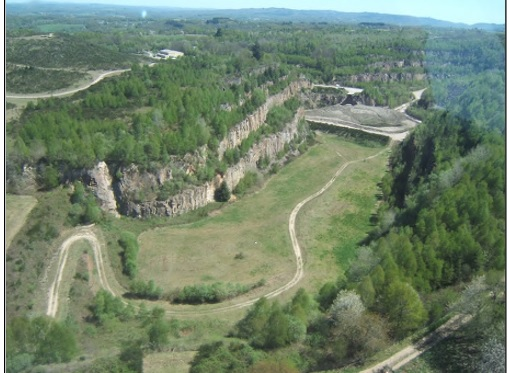
\includegraphics[width=0.4\textwidth]{I_A_3.jpg}}
%   \hfill
%   \subfloat[]{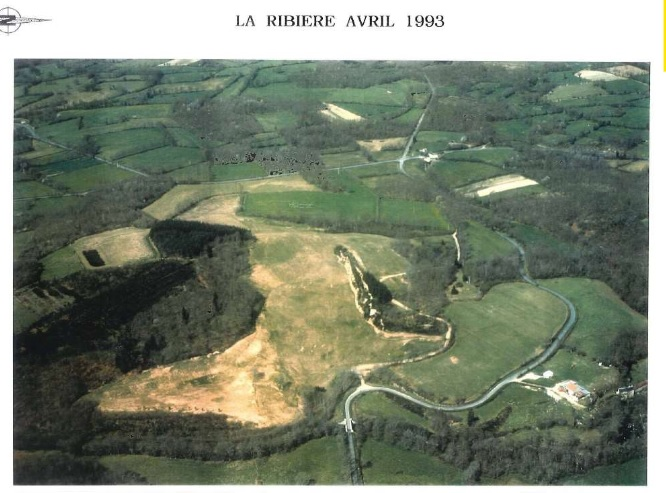
\includegraphics[width=0.4\textwidth]{I_A_4.jpg}}
%   \caption{}
% \end{figure}

\begin{figure}[H]
    \centering
    \begin{minipage}{0.5\textwidth}
        \centering
        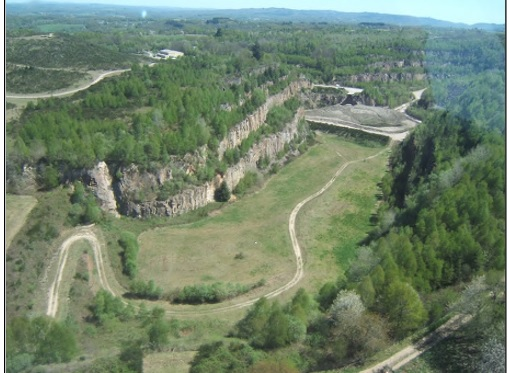
\includegraphics[width=0.9\textwidth]{I_A_3.jpg} 
        \caption{Site de Bellezane (Orano)}
        \label{fig:bellezane1}
    \end{minipage}\hfill
    \begin{minipage}{0.5\textwidth}
        \centering
        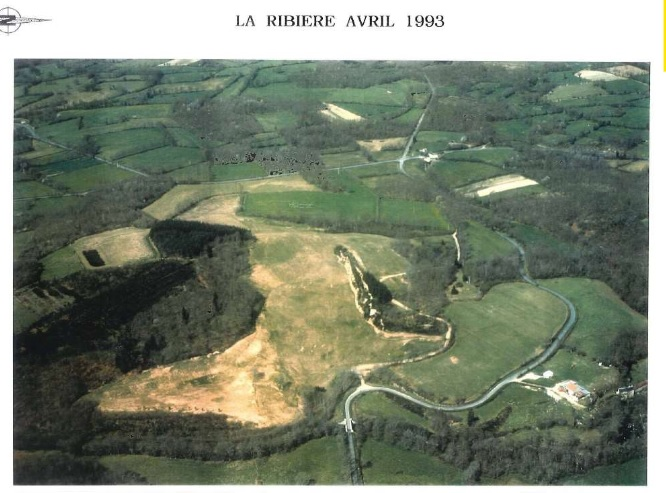
\includegraphics[width=0.9\textwidth]{I_A_4.jpg} 
        \caption{Site de La Ribière (Orano)}
        \label{fig:ribiere1}
    \end{minipage}
\end{figure}


A partir de 1967, le nombre de mines tend à décroître. Ce sont les mines de charbon qui disparaissent en premier, puis celles de bauxite, d’argent… À partir des années 1980, ce sont les mines d’uranium qui ferment massivement. Située à Jouac, non loin de Bessines, la dernière mine d’uranium française a fermé en 2001. Pour autant, cette date ne marque pas la fin de l’histoire des mines d’uranium en France. Il s’agit désormais de réaménager les sites de manière durable. C’est ce que l’on appelle l’après-mine.

%Annexe 1 Carte minière de la France 


\subsection{Importance et enjeux de l'après-mine}
\paragraph{} L’après-mine fait partie intégrante du cycle minier \cite{himeur_apres-mine_2020}. Aujourd’hui, cette phase est pensée dès les phases d’exploration et de développement du projet minier. C’est une étape clé qui comporte de nombreux enjeux. Elle dure en général plusieurs dizaines d’années, et il est nécessaire de surveiller la mine même au-delà. Il faut en effet assurer la sécurité et la salubrité de la mine.

L’objectif de ce processus est de réduire l’impact du site sur son environnement. Pour cela, il est essentiel de mettre en place un plan de réaménagement en concertation avec les autorités et les habitants. Une fois le plan établi et les différentes procédures achevées, les travaux peuvent commencer pour réinsérer le site dans le paysage. L’après-mine consiste aussi en la surveillance des sites. A l’issue du réaménagement, il faut continuer à entretenir les équipements de dépollution et vérifier que les normes sont toujours respectées.


%Image 1 (prez Après-mine Orano)
\begin{figure}[H]
    \centering
    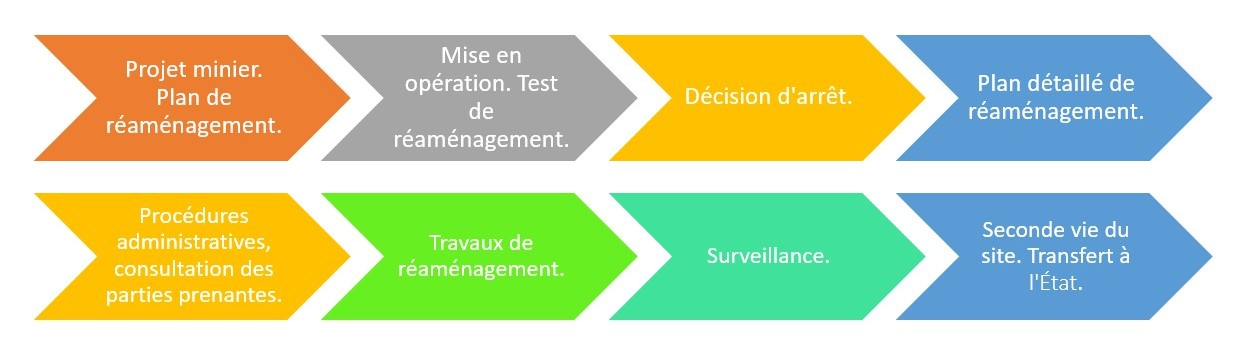
\includegraphics[width=\linewidth]{I_B_1.jpg}
    \caption{Les différentes phases du réaménagement d'une mine (Orano)}
    \label{fig:phases_reamenagement}
\end{figure}

La roche que l’on a excavé dans une mine pour atteindre le minerai constitue le stérile minier tandis que le produit issu du concassage du filon est appelé résidu minier. Ce dernier garde des propriétés radioactives : il faut donc le stocker et le surveiller.
Pour le réaménagement actif (remblayage), il s’agit souvent d’utiliser les stériles miniers pour remblayer les anciennes mines à ciel ouvert. On peut ensuite revégétaliser la zone - mais attention à ne pas planter d’arbres au-dessus des résidus, car leurs racines pourraient percer jusqu’à ces derniers. Il faut aussi s’assurer de ne pas forcer la nature, qui doit d’elle-même reprendre ses droits. Cela peut alors prendre 6 mois comme au Gabon, ou près de 10 ans comme près de Clisson en France où une forêt maritime est en train de se former. La stabilité peut être assurée avec des digues, qui retiennent les eaux d’exhaure et/ou les résidus. Des contrôles des résidus sont effectués régulièrement ainsi que des analyses de concentrations de radionucléides (uranium, radium…) dans l’eau et l’air du site \cite{himeur_apres-mine_2020}.

Des stations de traitement des eaux sont souvent utilisées pour traiter les eaux d’exhaure, certaines avec des méthodes de filtration particulières sur résines échangeuses d’ions ou sur zéolites, ce qui sera abordé plus tard dans le document. Le pôle Recherche et Développement (R\&D) de l’exploitant (Orano pour la France) a un rôle à jouer en essayant d’innover, d’optimiser ce traitement et d’étudier l’impact de l’après-mine sur les écosystèmes pour le minimiser \cite{schick_les_2020}.

Les secondes vies des mines peuvent être diverses : certaines sont transformées en parcs photovoltaïques, en zones industrielles ou agricoles, en musée (comme le musée Uréka de Bessines-sur-Gartempes), en base nautique ou encore en parc.
Les projets de parc photovoltaïques sont effectués en partenariat, ou via des appels d’offres  \cite{himeur_apres-mine_2020}.

À Bellezane, de nombreuses procédures ont été lancées. Des résidus y ont été coulés avant d’y poser une couverture en stériles et terre, puis de commencer la revégétalisation. Il y a notamment sur le site des fourrés et des mares à protéger, un écologue passe donc annuellement sur le site. L’entreprise MISTRI s’est désormais installée dans les anciens locaux du site, et un projet de centrale photovoltaïque en partenariat avec Total est en cours : il devrait aboutir vers 2023. Le stockage des résidus et sédiments marqués en radioactivité sur le site est, lui, géré par Orano \cite{benesteau_site_2020}.

%Image 2  : Bellezane avant/après
\begin{figure}[H]
    \centering
    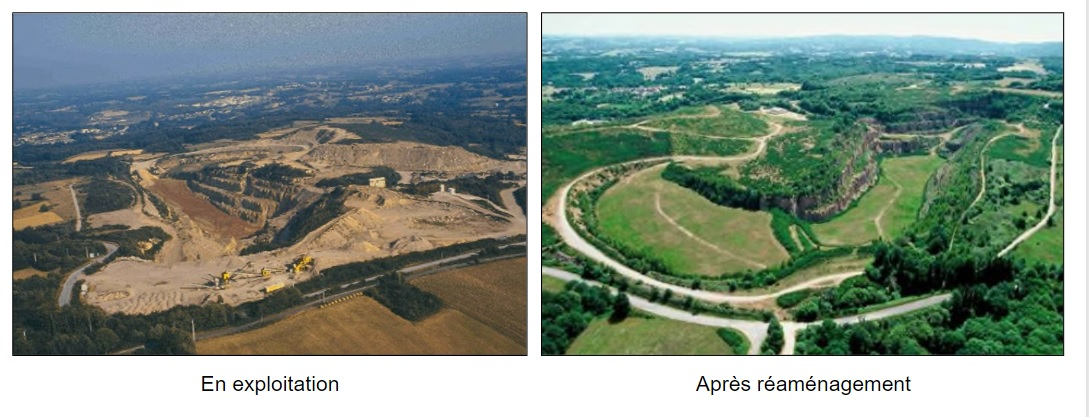
\includegraphics[width=\linewidth]{I_B_2.jpg}
    \caption{Le site de Bellezane avant et après le réaménagement (Orano)}
    \label{fig:bellezane_avant_apres}
\end{figure}

L’après-mine comprend une dimension sanitaire : les eaux d’exhaure peuvent se déverser dans des lacs ou des nappes utilisés pour le pompage de l’eau potable. C’est le cas par exemple dans le Limousin : les eaux d’exhaure de l’ancienne mine Henriette se déversent dans l’étang de la Crouzille qui est utilisé par la régie de l’eau de la métropole de Limoges pour alimenter le réseau d’eau potable. L’entreprise chargée de l’après-mine, Orano, doit donc veiller à la qualité de l’eau rejetée dans l’étang, qui ne doit pas dégrader la qualité de l’eau de l’étang. La présence de mines est également source de contraintes pour la régie de l’eau : la teneur en métaux et en minéraux de l’eau est modifiée par les eaux d’exhaure ce qui occasionne des frais de surveillance et de traitement supplémentaires. De plus, la disponibilité de l’eau est parfois réduite. Les mines ont également des effets indirects : elles ajoutent des contraintes de gestion technique et suscitent la méfiance des populations à l’égard des gestionnaires de l’eau \cite{vialleseche_station_2020}.

En raison des différents risques, notamment sanitaires, l’après-mine fait l’objet d’une réglementation. Celle-ci s’est développée en France dans les années 1970.
 La police des ICPE régie le stockage des résidus et la RGIE (Règlement général des industries extractives) le réaménagement. Ce n’est pas tout : diverses commissions de suivi sont mises en place, en général une par an pour les sites principaux : elles informent le public - notamment les riverains - sur les activités de gestion des sites.
L’IRSN, l’Institut de Radioprotection pour la Sûreté Nucléaire, est un organisme public qui participe aussi à l’après-mine : il réunit des experts scientifiques sur la question, forme et enseigne à des élèves et informe le public. Orano participe également à des congrès, à des études locales et à des groupes de travail sur le sujet. Ces derniers peuvent réunir des acteurs de domaines très divers : Ministère de la Transition Écologique, exploitant (Orano), experts techniques de l’IRSN, du BRGM ou de Geoderis, élus locaux, société civile… Ils étudient différents scénarios en se basant sur des critères et sous critères environnementaux, sociétaux et techniques différents afin de prendre en compte les avis de tous les acteurs.

Des programmes sont aussi mis en place comme le Plan National de Gestion des Matières et Déchets Radioactifs (PNGMDR) qui fixe des objectifs pour l’après-mine. Reconductible tous les 2 ans ou plus, son objectif est d’éclairer les autorités sur le réaménagement et le traitement, tout en prenant en compte l’évolution des situations et les contraintes de maintenance et de gestion.  [IRSN]

Par ailleurs, des visites de sites, des présentations et des conférences sont organisées pour sensibiliser et informer le public. Un musée, baptisé Urêka et situé à Bessines-sur-Gartempes, a été inauguré en 2013 dans le but de retracer l’histoire de l’industrie minière uranifère dans le Limousin.

Pour Orano, les mines représentent actuellement près du tiers des activités en France mais cette activité minière consiste principalement à réaménager les sites. Orano est chargé de l’après-mine uranifère en France, ce qui correspond à la gestion de près de 237 sites. Cela représente donc un enjeu important pour Orano : 26 personnes se consacrent à temps-plein à cet après-mine à Bessines-sur-Gartempes, dans le Limousin. Pour l’entreprise, l’après-mine représente 6 millions d’euros de dépenses annuelles pour la surveillance et l’entretien auxquels s’ajoutent 3 à 5 millions d’euros d’investissement dans des projets d’améliorations. Il y a donc également un enjeu économique pour l’entreprise \cite{himeur_apres-mine_2020}. 

Orano investit dans des outils spécifiques à l’après-mine afin de permettre un gain d’efficacité, ce qui démontre son importance dans le cycle minier. Des Systèmes d’Information Géographiques (SIG) ont notamment été mis en place, comme ArcGIS. Ce logiciel équipe Orano Mining afin de faciliter les tâches des techniciens chargés de la surveillance des sites. Les relevés sont notamment beaucoup plus rapides et précis grâce à cet outil. Des formulaires disponibles dans le logiciel permettent de recenser en temps réel les anomalies constatées sur le site et s’assurer qu’elles sont résolues par les autres équipes. Les points de prélèvement d’analyses d’eau et d’air y sont aussi indiqués, et les relevés peuvent eux aussi être faits en temps réel. ArcGIS permet de plus d’afficher des zones en réalité augmentée et de guider l’acquisition des données. 

D’autres outils numériques ont été développés pour l’après-mine. CartOmines est une story map permettant d’afficher d’anciennes vues minières (galeries, descenderies…) pour les comparer aux vues actuelles, grâce à d’importantes géodatabases. [CartOmines] Collector permet de modifier des données cartographiques et même de visualiser les galeries des mines en 3 dimensions ou en coupe. Le logiciel ERICA est utilisé pour évaluer les risques générés par l’uranium. Enfin, les bases de données Prodata, ainsi que les logiciels HYTEC et CHESS, que nous avons eu l’occasion d’utiliser, sont des outils importants utilisés pour la modélisation géochimique, hydrochimique et hydrogéologique des sites miniers. Puisqu’ils permettent de gérer l’après-mine en temps réel, les outils ont une grande importance. C’est pourquoi un budget annuel de 100 000€ leur est alloué %\cite{}.
%[S. Gerland]

%Image 3 (Akkari, S., Willocquet, R., 2020)
\begin{figure}[H]
    \centering
    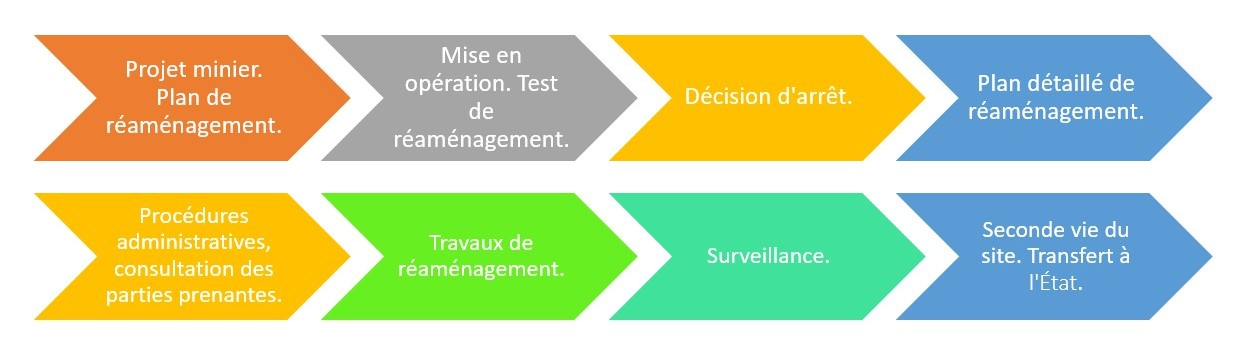
\includegraphics[width=0.9\linewidth]{I_B_3.jpg}
    \caption{Les différents acteurs de l'après-mine}
    \label{fig:acteurs_apres_mine}
\end{figure}

Ainsi, l’après-mine répond à de nombreux enjeux : il faut gérer les résidus et les stériles miniers, gérer les eaux d’exhaure, assurer la stabilité mécanique du site, surveiller l’impact radiologique, sans oublier la dimension sociale : le projet doit être accepté par les habitants et doit s’inscrire dans un projet de réhabilitation sur le long terme. Enfin, pour l’exploitant, il y a aussi une dimension économique.

\subsection{Enjeux sanitaires de l’après-mine}
\paragraph{Uranium}

Les différentes organisations de riverains et les acteurs publics en France se focalisent surtout sur la dangerosité de l’uranium. Pourtant, en ce qui concerne cet élément, il y a très peu d'études sur l’impact des mines sur la santé publique. Par exemple, au Québec, seulement 11 études sur l'impact sanitaire de l'élement uranium ont été retrouvées par l’institut national de santé publique du Québec, ce qui n’est pas suffisant pour donner de vraies conclusions sur les effets des résidus miniers. De plus, les études menées ne prennent parfois pas en compte le bruit de fond pour donner leur conclusion et sont donc inutilisables. 

Le \emph{bruit de fond} correspond à la radioactivité présente naturellement dans les roches. Elle varie selon les contextes géologiques. En France, afin d’étudier l’impact de l’uranium sur la santé humaine, l’IRSN se base sur des études sur l’influence d’un fort dosage d’uranium sur la santé des rats et a mis en évidence un effet délétère sur certains organes comme le cerveau ou les reins. 


Les sources les plus intéressantes de mise en évidence des effets sur la santé humaine proviennent d'études sur des individus étant régulièrement en contact de cet élément. Par ailleurs, des études sur les anciens mineurs ont mis en évidence que les cas de cancer du poumon étaient 127\% de fois plus élevés que la moyenne française. 

Il est avéré que l'uranium est à la fois chimiotoxique et radiotoxique. Les effets les plus importants sont observés au niveau des reins, avec atrophie tubulaire et amincissement du cortex rénal.

\paragraph{Radium}

Un autre résidu se retrouvant les résidus minier est le radium. Le radium est un élément radioactif donc il peut potentiellement être dangereux pour la santé. De plus, le radon est une autre source de pollution potentiellement dangereuse pour l’homme. Il est issu de la désintégration du radium, lui-même issu de la désintégration de l'uranium. Le radon est un gaz nocif pour l’humain. Les principales études sanitaires sur ce gaz ont été menées dans les années 1920. D’après elles, une exposition chronique au radium par ingestion peut causer non seulement des anémies mais aussi des cancers et une détérioration des tissus du squelette.

Plus récemment, l’IRSN a mené une étude sur le lien entre l’augmentation du taux de décès par cancer du poumon et la présence de radon dans les maisons. Les résultats ont été publiés en 2004 dans la revue « Epidemiology » [ Baysson et al 2004]. Ils montraient une augmentation faible du risque de cancer du poumon associée à l’exposition au radon  domestique. Cependant, les résultats sont très peu fiables étant donné qu’ils ont donné des résultats à la limite de la significativité statistique.  

\paragraph{Autres polluants}

Alors que l’on a tendance à se focaliser sur l’uranium et le radium dans l’étude des anciennes mines d’uranium, il ne faut pas oublier que l’on observe dans les mines la présence d'autres métaux qui peuvent être nocifs pour l’homme. Il y a par exemple le fer qui peut être trouvé à des concentrations assez élevées, lié à la présence d'oxydes de fer dans le milieu.  L'inhalation de concentrations excessives d'oxyde augmente le risque de développement de cancer du poumon, particulièrement pour les ouvriers exposés. Le plomb nuit également au système sanguin, au système nerveux, et au système rénal.

L’aluminium a quant à lui un impact sur le système osseux et sur le système nerveux. Cependant, d’après Santé Publique France, la détermination de l'impact sur la santé de l'exposition humaine à l'aluminium reste encore extrêmement difficile et source de nombreuses controverses. Une étude a été menée par l’Agence Française de Sécurité Sanitaire et a mis en évidence que l’aluminium pouvait avoir un impact négatif sur l’environnement et les hommes mais sans pouvoir définir précisément les impacts.  Par exemple, des effets neurologiques de l’aluminium sur l’humain ne se sont pas retrouvés avérés.

Ces polluants sont importants pour les entreprises et doivent être pris en compte pour le réaménagement des mines. Pour celà, de nombreux modèles hydrogéologiques sont mis en place pour quantifier la pollution. C'est que nous nous sommes proposé d'étudier dans cette deuxième partie. 

\newpage
\section{Problématique de l’après-mine}
\subsection{Les différentes pollutions}
\subsubsection{L'uranium}

\subsubsection{Le radon, un polluant gazeux issu des résidus de traitement}

\paragraph{Formation et émanation du radon}

\paragraph{} Les résidus de traitement, dont on a extrait l’uranium, contiennent encore des traces d’uranium et de radium, qui se situe dans la chaîne de désintégration radioactive de l’uranium (figure \ref{fig:desintegration_uranium}).

Au sein d’un grain de résidu, les atomes de radium, dont la demi-vie est de 1602 années, se désintègrent en atomes de radon en libérant une particule alpha. Alors que la radioactivité alpha de l’uranium ou du radium, libérée en profondeur, ne pose pas de risque radiologique direct, le radon naît à l’état gazeux et peut atteindre la surface. Il est donc impératif de savoir quelle proportion de radon est transportée vers la surface, pour évaluer les risques et prendre les mesures de sûreté nécessaires.

La première étape du transport du radon est appelée émanation. Le radium se désintègre au sein des résidus de traitement, qui sont sous forme de grains, et ainsi, tous les atomes de radon ne parviennent pas à atteindre les porosités. En effet, la distance $R_s$ que les atomes peuvent parcourir de l’ordre de 30 nm dans un minéral de densité commune. Cette distance est de 50 $\mu$m dans l’air et de 50 nm dans l’eau.

On définit alors le facteur d’émanation comme étant la proportion d’atomes de radon qui atteignent les porosités sans être absorbés par un autre grain. Il est possible d’estimer le facteur d’émanation \cite{fleischer_theory_1983} dans le cas simplifié d’un grain sphérique de diamètre D, sans prendre en compte l’humidité ou la potentielle absorption des atomes par un grain adjacent (détails en annexe B\ref{annexe:emanation}). La littérature scientifique \cite{ferry_migration_2000} permet de confirmer l’ordre de grandeur obtenu par le calcul simplifié à sec pour des grains dont le diamètre est de l’ordre du micromètre ($E \simeq 10^{-2}$). On note que le facteur d’émanation est d’autant plus élevé que les résidus sont humides ($E\simeq 0,3$) puisque l’eau, avec une distance d’arrêt plus courte, empêche les atomes d’être absorbés par les grains adjacents.

Pour nos valeurs numériques dans les résidus miniers, enfouis en zone saturée, on a sélectionné une valeur du coefficient d’émanation $E=0,3$.

\paragraph{Équilibre séculaire}

\paragraph{} Au sein des résidus, le radium se désintègre en radon, mais le radon se désintègre également, plus rapidement. Au bout d’un certain temps, autant de radon est créé que désintégré. La concentration de radon dans les résidus est alors constante, c’est l’équilibre séculaire.

On peut déterminer l'activité volumique du radon $a_0$ (en $Bq/m^3$) dans les résidus atteinte à cet équilibre, en fonction de l'activité massique du radium $A_{Ra}$ ($Bq/kg$), du facteur d'émanation $E$ du milieu, de sa masse volumique $\rho$, de sa porosité $\omega$ et de sa une saturation en gaz $S_g$ (détails et valeurs sélectionnées en annexe B\ref{annexe:seculaire} :
$$
a_0 =\frac{E(1-\omega)\rho}{\omega S_g} A_{Ra} =9,1 \; \text{MBq/m}^3
$$

\paragraph{Transport du radon vers la surface}

\paragraph{} Plusieurs processus peuvent expliquer le transport du radon vers la surface \cite{irsn_ineris_radon_nodate} : sa diffusion ou le déplacement de la matière environnante.

Le moteur de la diffusion du radon dans les pores est son gradient de concentration, dans la mesure où le radon est transporté vers les zones où sa concentration est plus faible. Par ailleurs, le radon étant un gaz inerte, dense et très dilué, son transport est surtout lié au mouvement de son environnement, c’est-à-dire d’autres gaz ou l’eau infiltrée dans le sous-sol. Le gradient de température est le moteur de la convection de ces fluides, mais c’est surtout le gradient de pression - le moteur de l’advection - qui induit une vitesse de Darcy et qui engendre le transport du radon. Autrement dit, si l’eau est en mouvement, le radon emprisonné dans l’eau se déplace avec elle.

\paragraph{Impact radiologique : calcul de dose efficace}

\paragraph{} Le radon gazeux, à l’air libre, est susceptible d’être inspiré par des êtres humains. Sa désintégration de type alpha pose alors un risque radiologique important. Son impact a donc été quantifié par plusieurs agences de radioprotection, et des normes ont été imposées.

Il y a tout d’abord une norme sur la dose efficace de radioactivité absorbée. En France, la dose efficace moyenne liée au radon est de 1,43 mSv/an (figure \ref{fig:exposition_moyenne}) \cite{irsn_quelle_nodate}. Cette exposition est en partie d’origine naturelle, puisque le radon est un élément chimiquement présent dans les sols, notamment dans les zones granitiques. En revanche, l’exposition au radon peut également être d’origine anthropique, et c’est là qu’intervient la norme \cite{inrs_rayonnements_nodate}. La valeur limite d’exposition du public ou des travailleurs non exposés au radon est de 1 mSv, et de 20 mSv pour les travailleurs majeurs exposés (figure \ref{fig:comparaison_normes}).

Depuis le 1er juillet 2018, le niveau de référence de l’activité volumique du radon dans l'air est fixé à $300 \; Bq/m^3$ en moyenne annuelle \cite{autorite_de_surete_nucleaire_reglementation_nodate}, dans les bâtiments habités, publics ou accueillant des travailleurs. Il est possible de déduire la dose efficace d’exposition au radon sur le lieu de travail à partir de l’activité volumique en radon $a$ en $Bq/m^3$, le temps de travail en heures $\Delta t$ et du facteur d’équilibre $F$, qui est une image de la qualité de la ventilation du milieu. Un facteur d’équilibre proche de $0$ caractérise un milieu bien aéré, et un facteur d’équilibre proche de $1$ signifie que l’air du milieu n’est que très peu renouvelé. Le facteur d’équilibre $0,4$ correspond à la moyenne dans les habitations françaises. Une ventilation forcée peut baisser ce paramètre. L'INRS donne alors une expression \cite{blanchardon_evaluation_2019} de la dose efficace (en Sieverts) :
$$
d = r F a \Delta t
$$
Où $r=7,8 \; .10^{-6} \; mSv/(Bq/m^3.h)$ est un coefficient lié à l’impact du radon, que l'on approxime en annexe B\ref{annexe:estimation_r}.

La figure (II-Ab-6) permet de visualiser la position du niveau de référence de $300 \; Bq/m^3$ par rapport aux limites d’exposition (les cases rouges sont les doses dépassant la limite légale de dose efficace) pour des travailleurs qui ont travaillé 35 heures pendant 56 semaines de l’année. On note que le niveau de référence est bien positionné.

\begin{figure}[H]
    \centering
    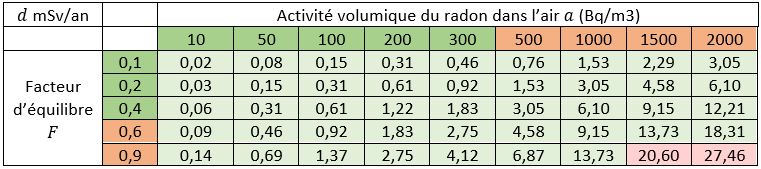
\includegraphics[width=\linewidth]{II_A2_6.png}
    \caption{Dose efficace en $mSv/an$ en fonction de $F$ et $a$ pour un travailleur}
    \label{fig:exposition_double_entree}
\end{figure}

A la surface de la zone d’enfouissement des résidus de la Ribière, on peut approximer analytiquement la valeur de l’activité volumique à $a=180 \; Bq/m^3$. Pour une ventilation naturelle $F=0,4$ et 56 semaines de travail à 35h, la dose efficace absorbée par un travailleur est de $1,1 \; mSv$. Cette valeur respecte les normes établies par le code du travail.

\subsection{La dimension sociétale}
\subsubsection{La prise en charge des tensions entre riverains et entreprises}
\paragraph{} De nos jours, des tensions sont encore présentes entre ORANO et les riverains. Le manque d’informations transmises par COGEMA (l’ancien nom d’ORANO) lors de l’ouverture des mines a rendu la population locale méfiante envers les différentes actions que l’entreprise a prises pour enfouir les déchets radioactifs. Les organisations locales, comme l’association Source et Rivière du Limousin, se tournent alors vers des organisations à but non lucratif pour accéder à des informations fiables sur les sites. 

L’une de ces organisations est la CRIIRAD (Commission de Recherche et d'Information Indépendantes sur la Radioactivité). Cette association, créée en 1986, agit pour un accès plus direct à l’information sur la radioactivité à l’aide d’un laboratoire de recherche indépendant. Dans les années 90, elle décide de se tourner vers la surveillance des anciens sites miniers à la demande d’acteurs locaux qui doutent des informations transmises par ORANO. Le but initial de la CRIIRAD est de faire des constats sur les sites en prélevant des échantillons, puis de former des citoyens à continuer cette surveillance. Ensuite, un dialogue s'instaure avec les différents partis concernés, comme les entreprises en charge du réaménagement, des CSS (comité de suivi des sites) ou d’autres acteurs comme l’IRSN. Suite à ce dialogue, les mines peuvent passer ICPE (Installation Classée pour la Protection de l'Environnement) où l’exploitant se voit obligé d’apporter des mesures complémentaires au site. Cependant, un enjeu économique entre en jeu lors de la demande de travaux complémentaires, qui peuvent donc ne pas être aussi efficaces que l’espèrent les organisations locales. 

Pour poursuivre la surveillance des sites sur des périodes de temps plus longues, la CRIIRAD a mis en place un Collectif Mines d’Uranium (CMU). Le CMU (regroupant plusieurs associations dont l’Association Oui à l'avenir (Creuse), l’Association Noria (Vendée), l’Association Sources et Rivières du Limousin (SRL), et bien d’autres) déplore  l’état dans lequel les entreprises minières laissent le territoire et  affirme que les déchets miniers sont souvent « disséminés dans l’environnement ou stockés dans des conditions totalement inappropriées » et qu’ils « génèrent des pollutions environnementales multiples (air, eau, sol, chaîne alimentaire) induisant des dangers sanitaires inacceptables aujourd’hui et pour les générations futures ». Il tiennent ORANO pour responsable de la dégradation de la faune et de la flore et protestent contre une « législation complaisante ». Ils se plaignent, entre autres, de la contamination des terrains par des éléments radioactifs, de la pollution des ressources aquatiques, de la mauvaise gestion des sites de stockage des déchets, de la perte de mémoire sur la localisation des sites, de l’absence de normes sanitaires et environnementales intégralement respectées… Accompagnés de la CRIIRAD, ils reprennent les rapports d’ORANO et de l’IRSN pour en dégager les erreurs et avoir un impact assez important pour que les acteurs publics agissent.

Cependant, même avec l’action de la CRIIRAD, certains maires ou organisations territoriales se trouvent impactées par la mauvaise gestion de l’Après-Mine. L’impact sur le tourisme et l’accès au ressource n’est pas négligeable, puisqu’il est impensable de construire un complexe sur un ancien site minier, ou de se servir de l’eau d’un lac pollué pour l’agriculture par exemple. AREVA ayant laissé les entreprises utiliser les stériles miniers pour différents projets, il faut aussi détruire des infrastructures qui présentent un danger radioactif.


\subsubsection{Gestion des risques par un acteur extérieur: le rôle de l’IRSN}
Plus spécifiquement en ce qui concerne les risques liés à la radioactivité, l'Institut de Radioprotection et de Sûreté Nucléaire (IRSN), est un Établissement Public à caractère Industriel et Commercial créé en 2001 qui fonctionne sous la tutelle conjointe des ministères de la Défense, de l’Environnement, de la Recherche de la Santé. Il s’agit de l’expert français en matière de recherche et d’expertise sur les risques nucléaires et radiologiques. L’IRSN s’intéresse à l’impact radiologique sur la santé et sur l'environnement et intervient dans la gestion de la sûreté et de la sécurité nucléaire.  Lors de la prise en charge d’un projet comportant un risque radiologique, l’IRSN, les concepteurs ou constructeurs, les autorités publiques et les parties prenantes (comme les Commissions Locales d’Informations) sont en interaction mutuelle.

L’IRSN s’occupe donc  du réaménagement des anciennes mines d’uranium en France. Pour ce faire, l’institut doit tout d’abord connaître l’impact radiologique de l’ancienne mine sur l’environnement et sur les populations. Le modèle ERICA (méthode d’évaluation du risque environnemental associé aux rejets de substances radioactives mise en place dans le cadre du projet européen ERICA) est utilisé pour déterminer  le risque environnemental en effectuant des mesures dosimétriques sur le terrain. L’objectif est de quantifier la probabilité de l’existence d’un risque potentiel sur les écosystèmes aquatiques.

L’institut  mène  des  expertises  afin  d’évaluer  des  points  techniques  particuliers,  concernant notamment l’impact radiologique de certains sites. Lorsqu’elles sont réalisées à la demande des préfets, les interventions de l’IRSN prennent en général la forme de tierces expertises, portant sur les documents techniques produits par ORANO au sujet des travaux qu’il mène sur  ses  sites  ou  de  l’impact  environnemental  de  ceux-ci.

Pour les sites miniers, l’enjeu est le long terme: les polluants seront là pendant des dizaines de milliers d’années. Les réglementations qui s’appliquent sur ces sites sont le code de la santé publique, pour la protection du public contre les rayonnements ionisant autour des anciens sites miniers d’uranium; le code minier, pour la partie exploitation, surveillance et réaménagement; et le code de l’environnement, pour le stockage des résidus.

L’objectif pour les entreprises est de faire en sorte que les eaux rejetées dans l’environnement   soient conformes aux limites fixées par arrêté préfectoral. Il est  basé sur les limites fixées par le RGIE (Règlement Général des Industries Extractives).

Au niveau sanitaire, l’impact radiologique sur la santé a été évalué par la Commission Internationale de Protection Radiologique qui a évalué le risque à 17 cancers pour 100 000 personnes exposées à 1 mSv/an. La limite fixée pour le public est de 1 mSv/an et pour les travailleurs miniers de 20 mSv/an. Or, certains acteurs comme des associations pour les travailleurs au Niger ou les Amis de la Terre en France dénoncent Orano pour ne pas avoir admis mettre en danger ses travailleurs en les exposant à 20 mSv/an. Selon eux, d’une part les études scientifiques ne sont pas précises et donc Orano n’est en rien obligé de se plier aux seuils définis par la CIPR et d’autre part Orano ne prend pas en compte dans ses calculs les émissions radiologiques liées au fond géochimique lorsque le travailleur rentre chez lui.

\subsection{Les différentes normes mises en place sur l’eau}
\subsubsection{Acteurs de la législation}
\paragraph{} De nombreux acteurs interviennent dans la mise en place d’une législation régissant la qualité des eaux. Tout d’abord, c’est l’Union Européenne qui établit des directives. Les états-membres doivent transposer ces actes juridiques dans leur législation nationale. En France, le  ministère de l’environnement contrôle le Comité National de l’Eau, qui évalue la qualité et le prix de l’eau, et l’Office National de l’Eau et des Milieux Aquatiques  qui contrôle les usages des milieux aquatiques. Il existe aussi des institutions régionales : la direction régionale de l’environnement, de l’aménagement et du logement, l’agence régionale de santé et la direction départementale du territoire  appliquent les directives nationales dans les différents régions. De manière encore plus locale, les collectivités territoriales (communauté de communes ou d’agglomérations, métropoles) donnent des ordres pour les travaux de Gestion des Milieux Aquatiques et de Prévention des Inondations. Enfin, les acteurs économiques et les diverses associations de protection de l’environnement entrent en jeu : les industriels et les agriculteurs sont responsables de leurs installations de dépollution et de prélèvement. Parallèlement, les associations sont associées aux décisions au sein du Comité de bassin, appliquées par l’agence de l’eau.

\subsubsection{Cas de l’eau rejetée dans l’environnement}
Lorsqu’il n’est pas nécessaire que l’eau soit potable, la DCE (Directive-Cadre sur l’Eau) est la directive européenne qui fait loi. Adoptée en 2000 pour préserver la ressource en eau, elle indique des valeurs seuils pour protéger la vie humaine mais aussi l’environnement. Les NQE (Normes de Qualité de l’Eau) sont définies dans la DCE au niveau européen pour les substances polluantes prioritaires. La NQE est la plus faible des PNEC (“Predicted No Effect Concentration”) : concentration en dessous de laquelle aucun effet inacceptable n’est observé. Ces NQE n’étant définies que pour les polluants considérés comme prioritaires, des VGE (Valeur Guide Environnementale) ont été établies: elles sont calculées comme les NQE mais n’ont pas de valeur réglementaire (donc ne sont pas obligatoirement respectées).

Pour définir ces normes, il faut notamment prendre en compte le fond géochimique. Le fond géochimique est la composition chimique d'un sol et des roches du sous-sol dont il est la décomposition. Il détermine en partie la qualité du sol, de l'eau et la vie de la flore et de la faune. On distingue généralement le fond géochimique naturel, résultant exclusivement de l'évolution de la roche-mère et d'apports naturels : salinité, confinement d’une eau, phénomène de drainance, et le fond d'origine anthropique, qui exprime la part des éléments exclusivement introduits dans le milieu par les activités humaines ou à la suite de ces activités. Le fond géochimique naturel est parfois confondu avec le  “bruit de fond”, mais ce dernier comprend également des apports anthropiques diffus. Les substances généralement considérées pour l’évaluation d’un fond géochimique sont  l’arsenic, le baryum, le bore, le fluor, le cadmium, le chrome, le mercure, le cuivre, le nickel, le plomb, le zinc, l’antimoine, le sélénium, l’aluminium, l’argent, le fer et le manganèse.

Pour quantifier la quantité de polluants dans le milieu, les différents acteurs ont besoin de connaître le fond géochimique du milieu afin de savoir s’ils dépassent sa valeur pour les polluants lors du rejet des eaux dans l’environnement. Or, ce bruit de fond géochimique est difficile à quantifier car il dépend du milieu, et au sein d’un même site sa valeur peut varier d’un point à un autre. Les acteurs ont alors du mal à quantifier la quantité de polluants qu’ils rejettent dans l’environnement et peuvent parfois dépasser les valeurs seuils en prenant en compte une valeur de bruit de fond géochimique plus importante. De plus, la proportion naturelle en certains éléments est parfois supérieure à celle fixée par la législation. C’est en France le cas du baryum (concentration maximale naturelle de 1600 mg/L alors que la norme est à 700 mg/L), du fluor (12 g/L contre 1.5 g/L) ou encore du nickel (100 mg/L contre 20 mg/L) par exemple. D’où la difficulté à établir des normes qui puissent être respectées partout. %/ cf tableau

Un autre moyen pour établir l’impact de la pollution des eaux de surface sur l’environnement est d’étudier la faune et la flore du milieu. Cela pose un problème car les effets sont donc observés après la pollution du milieu et peuvent ne pas être pris en compte par les entreprises. 

\subsubsection{Cas de l’eau potable} 

\paragraph{} Lorsque l’eau est destinée à la consommation humaine, les critères de potabilité sont établis sur la base des recommandations en vigueur de l’Organisation Mondiale de la Santé (OMS) et sur celle de données scientifiques établissant des doses maximales admissibles (DMA), définies comme la quantité maximale d’une substance qu’une personne peut absorber tous apports confondus (alimentaires, hydriques), sans danger, chaque jour, sa vie durant. Ces doses sont calculées pour des personnes fragiles (bébés, femmes enceintes, immunodéprimés).

Ces critères sont basés sur les principaux indicateurs de la qualité de l’eau. Ils indiquent les  germes pathogènes, virus et bactéries, micro-organismes parasites ainsi que les autres polluants chimiques à éliminer, et de même quels sels minéraux et quels oligo-éléments sont à conserver (comme le calcium, le magnésium, le chlore ou le fer). Afin de fixer une réglementation adaptée, une différence fondamentale est établie entre références de qualité et normes de qualité: les normes de qualité, impératives, concernant des substances pouvant avoir une répercussion sur la santé tandis que les références de qualité (couleur, odeur) sont des indicateurs reflétant le bon fonctionnement des installations de production d’eau potable.
La qualité de l’eau potable est encadrée par une réglementation européenne, le Code de la Santé publique, des décrets, des arrêtés, des circulaires et en particulier par la Directive européenne 98/83 du 3 novembre 1998 et par  le décret 2001-1220 qui fixe les limites et références de qualité pour l’eau potable. Plus spécifiquement, en France, le code de santé publique (CSP) régit le socle de la réglementation en matière de qualité, de production et de distribution de l’eau et transpose les directives européennes. 

\subsubsection{Comparaison avec d’autres pays}

\paragraph{Australie}

En Australie, les \textit{Environmental Requirements} (ER) pour la mine d’uranium de Ranger, établis en 1999, fixent les normes de protection environnementale auxquelles l’entreprise responsable d’un site minier doit se soumettre. L’entreprise doit s’assurer que les opérations minières ne compromettent pas l’écosystème environnant et la santé de la population locale. Elle doit maintenir la biodiversité des écosystèmes et assurer la continuation des processus biologiques. Elle doit par ailleurs réhabiliter le site minier de sorte à établir un environnement correspondant à sa zone géographique, en assurant la revégétalisation avec des espèces natives de cette zone, avec la même densité et abondance, ou encore en faisant en sorte que les caractéristiques d’érosion du site soient cohérentes, afin d’assurer la viabilité à long terme et, à terme, de permettre à la zone de se développer sans maintenance particulière par rapport aux zones alentour. De plus, l’entreprise doit assurer des conditions radiologiques stables afin que la dose reçue par les travailleurs et le public soit aussi basse que raisonnablement possible. Elle doit pour cela minimiser le volume d’eau contaminée nécessaire pour faire fonctionner le site, et minimiser la quantité de contaminants présente dans cette eau, tout en s’assurant que ces contaminants soient contenus dans le site. De même, les émissions gazeuses et particulaires doivent être minimisées. L’objectif étant de limiter autant que raisonnablement possible les risques pour la santé des locaux. L’entreprise doit pour cela suivre le principe BTP (\textit{Best Practicable Technology}), en implémentant la technologie disponible ayant le plus de retombées positives sur l’environnement. L’Australie a donc mis en place un mode de gestion ALARA (\textit{As Low As Reasonably Possible}) pour le contrôle et la réhabilitation de ses mines d’uranium.
Les mesures correctives doivent être prises en accord avec le ministère de l’environnement, mais ce sont les compagnies minières qui ont la responsabilité de réaliser la réhabilitation et de payer les coûts associés jusqu’à ce que les autorités (comme par exemple le \textit{Northern Territory Department of Mines and Energy} : NTDME) estiment que le site a été réhabilité à un niveau satisfaisant. La surveillance du site doit par ailleurs s’effectuer par des prélèvements réguliers sur les eaux souterraines.

\paragraph{Allemagne}

En Allemagne, le \emph{Radiation Protection Act} (StrlSchG), établi en 2017, fournit le cadre juridique de la protection face aux effets néfastes des radiations et établit les bases légales de la radioprotection. Cet acte implémente la directive 2013/59/Euratom du conseil européen qui met en place des standards de protection face à l’exposition aux radiations. Cet acte met donc en place des valeurs limites de concentration d’activité, d’activité et de dose effective annuelles précises pour des espèces radioactives et des publics distincts. 


Par exemple, la limite générale de la dose effective annuelle pour le public est de 1 mSv, et la concentration d’activité de l’uranium ne doit pas dépasser 10 kBq/kg. Cependant, il n’existe pas de loi spécifique à la gestion des mines d’uranium après la fin de leurs activités, pas de législation globale sur les méthodes à appliquer. Le gouvernement allemand préfère appliquer des méthodes distinctes pour chaque site afin d’apporter des réponses adaptées à des questions spécifiques.

La réhabilitation des mines d’uranium allemandes est principalement gérée par la société Wisbut GmbH, détenue et financée par le gouvernement. Elle est chargée du démantèlement des mines, du traitement du site et de la surveillance des installations et des émanations. La surveillance implique des mesures menées sur le long terme à des positions précises afin d’assurer la cohérence du site avec la loi et un meilleur contrôle sur les actions de réhabilitation.

\paragraph{Etats-Unis}

Aux États-Unis, en 1950, le \textit{US Public Health Service} commençait une étude sur les mineurs d'uranium, conduisant à la première publication d'une corrélation statistique entre le cancer et l'extraction d'uranium, publiée en 1962. Le gouvernement fédéral a finalement réglementé la quantité standard de radon dans les mines, fixant le niveau à 0,3 WL en 1969. 

Plus tard, l'USAEC (\textit{United States Atomic Energy Commission}) a donné l’objectif et des conseils pour la réhabilitation de l’eau dans les anciens sites miniers, surtout pour les eaux souterraines contaminées par l'ISR. L’objectif est de restaurer la qualité de l'eau dans les nappes aquifères affectées à l’état avant l'exploitation minière. Bien que toutes les caractéristiques chimiques ne puissent pas être retournées à celles avant l'extraction, l'eau doit être assurée aux mêmes utilisations qu'auparavant. 

L'USAEC formule des recommandations concernant la caractérisation du niveau de base (baseline) de la qualité des eaux souterraines avant le début des opérations minières, la surveillance pour détecter l’évolution de lixiviat pendant l'exploitation minière et la surveillance à long terme pour déterminer à quel moment la qualité des eaux souterraines se stabilise après la fermeture des opérations minières.

L'eau avant l'exploitation est généralement de mauvaise qualité (teneurs élevées en métal, en uranium et parfois de haute salinité), résultant des mécanismes de genèse du minerai. L'objectif de qualité physico-chimique à atteindre dépend de la réglementation locale, généralement de concentration aussi proche que possible du niveau de base.

Par exemple, au Texas, c’est la TCEQ (\textit{Texas Commission on Environmental Quality}) qui définit le niveau de base pour ses sites miniers locaux et surveille la réhabilitation. Le tableau suivant résume les données de référence des eaux souterraines avant l'extraction. Au Texas, 26 éléments chimiques sont mesurés avant l'exploitation minière pour établir le niveau de base, qui est l’objectif initial de restauration. On sélectionne la concentration moyenne la plus élevée de la zone de mine. Dans le site Zamzow, 0,171 milligramme par litre d'uranium était la valeur moyenne la plus élevée de cette zone.

%Figure 2 – Niveau de base du site Zamzow
\begin{figure}[H]
    \centering
    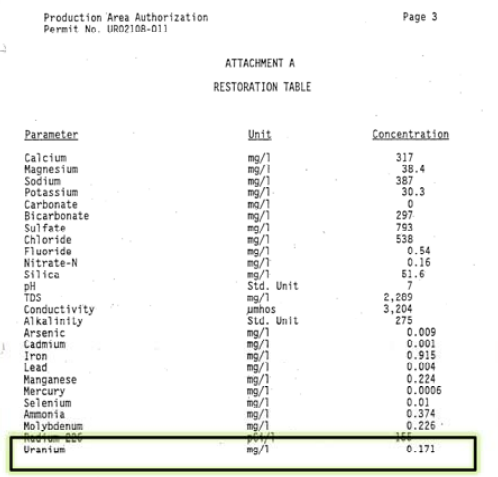
\includegraphics[width=0.8\linewidth]{II_C_2.png}
    \caption{Niveau de base du site Zamzow}
    \label{fig:site_zamzow_base}
\end{figure}

Cependant, une étude publiée par l'\textit{U.S. Geological Survey} en 2009 a révélé que « À ce jour, aucune opération après ISR aux États-Unis n'a réussi à restaurer l'eau dans l'aquifère au niveau de base ». Tous les sites du Texas ont reçu des objectifs de restauration modifiés pour au moins un élément, déterminés par TCEQ. Les données de restauration finale pour Zamzow montrent une limite modifiée de 3,00 milligrammes par litre pour l'uranium. 


%Figure 3 - Données de restauration finale du site Zamzow
\begin{figure}[H]
    \centering
    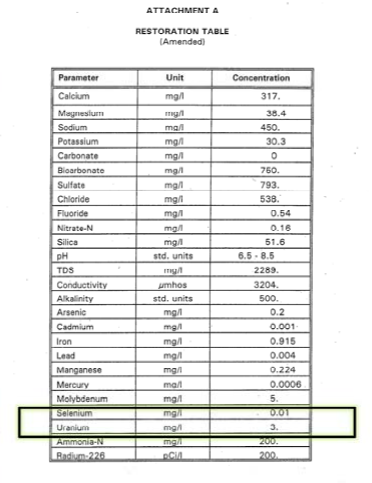
\includegraphics[width=0.7\linewidth]{II_C_3.png}
    \caption{Données de restauration finale du site Zamzow}
    \label{fig:restauration_finale_zamzow}
\end{figure}


Ce graphique de concentration d'uranium pour divers sites du Texas illustre la relation entre les niveaux de base, les valeurs finales après réhabilitation et les objectifs de restauration modifiés. Les barres bleues représentent les niveaux de base. Les barres rouges représentent les concentrations finales pour l'uranium, et les barres vertes représentent les objectifs de restauration modifiés par TCEQ.

%Figure 4 - Concentration d'uranium pour divers sites du Texas

\begin{figure}[H]
    \centering
    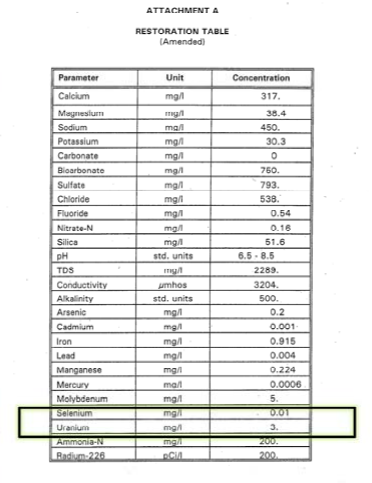
\includegraphics[width=\linewidth]{II_C_3.png}
    \caption{Concentration d'uranium pour divers sites du Texas}
    \label{fig:conc_u_texas}
\end{figure}

\newpage

\paragraph{Canada}

Le Canada est un État fédéral et la responsabilité de la réglementation de traitement et la réhabilitation est partagée entre les gouvernements provincial et fédéral. Le 30 juin 1996, la dernière mine de la région d'Elliot Lake, la mine Stanleigh, était fermée. Après, seule la province de la Saskatchewan produit de l'uranium, mais comme la teneur en uranium du gisement de la Saskatchewan est élevée, le Canada restera le plus grand producteur d'uranium au monde.

L'AECB (\textit{Atomic Energy Control Board}), un organisme indépendant du gouvernement du Canada, est responsable des affaires liées à l'énergie nucléaire et aux matières radioactives. Le règlement R-90 traite de la fermeture et de la réhabilitation des sites. Bien que le Canada réglemente les mines d'uranium, les provinces sont les principaux propriétaires fonciers. Par conséquent, les mines d'uranium fermées reviendront finalement aux provinces ou redeviendront des terres de la Couronne. Les agences environnementales provinciales sont les principaux régulateurs de la qualité de l'eau de tous les sites miniers.

En 1996, l'AECB a établi la réglementation stratégique de gestion des déchets radioactifs pour s'assurer que les déchets après les mines sont gérés de manière responsable. Les objectifs de cette réglementation canadienne sont :
\begin{itemize}
    \item protéger l'environnement, en tenant compte des facteurs sociaux et économiques
    \item minimiser le besoin de contrôle et de surveillance à long terme
    \item s'assurer que les risques pour la santé sont conformes aux normes en vigueur 
    \item ne pas interdire l'utilisation future des ressources naturelles contenues dans les déchets miniers.
\end{itemize}

Cela signifie en fait que des normes spécifiques sont développées, dépendant des situations actuelles de chaque site. Néanmoins, un certain nombre de critères communs sont applicables à tous les sites. Par exemple, une valeur de 1 mSv par an pour l'équivalent de dose efficace moyen est à respecter sur une période de 50 ans après la fermeture des sites d'uranium, ainsi que les autres exigences légales sur la sécurité nucléaire et la protection radiologique mises en place par l'AECB.

Dans ce cadre, les propriétaires des déchets sont responsables du financement, de l'organisation, de la gestion et de l’élimination des installations. Pour les anciennes mines d'uranium, dont beaucoup ont été fermées il y a plus de 50 ans, plusieurs facteurs doivent être pris en compte. Dans de nombreux cas, l'entreprise qui exploitait la mine, ou son successeur, existe toujours et s'occupe des déchets sur ses sites. Cependant, dans certains cas, le site est retourné à la Couronne lorsque les entreprises n’existent plus et alors la responsabilité de traitement des déchets est partagée entre les gouvernements provincial et fédéral. Lorsque ces anciennes mines fonctionnaient, les réglementations environnementales appliquées à l'industrie minière n'étaient pas très strictes. Cependant, il n'est pas souvent pratique ou rentable de remettre en état les anciens sites en respectant les normes actuelles. La plupart des sites présentent un risque très faible, en raison des faibles teneurs de minerai, de leurs emplacements éloignés et du fait que les polluants se sont dissipés au cours des 50 dernières années.

\newpage
\section{Traitements/Solutions}
\subsection{Les différentes méthodes de traitement des eaux}
Le traitement des eaux en sortie de mines est ainsi un enjeu central de l’après-mine. En France, plusieurs techniques de traitement sont utilisées dans les quinze stations stations dédiées. Elles diffèrent par les installations qu’elles requièrent tant que par leurs implications socio-économiques.

\subsubsection{Fonctionnement et coûts}
\paragraph{Traitement par précipitations} \hspace{1 em}

%(IMAGE $III_A_1$)
\begin{figure}[H]
\centering
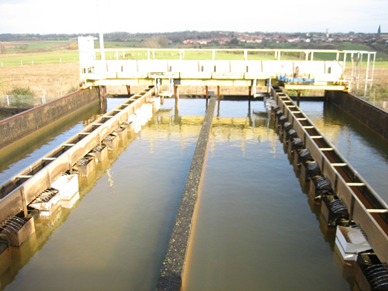
\includegraphics[width = 0.5\linewidth]{III_A_1.png}
\caption{Bassin de décantation}
\label{fig:bassin_decantation}
\end{figure}

Le procédé de traitement des eaux le plus répandu en France est le traitement actif par précipitation et coagulation-floculation-décantation. Il équipe onze des quinze stations de traitement des eaux de sortie de mine d'uranium françaises. 
L’étape de précipitation vise la transformation des métaux dissous dans l’eau (généralement fer, aluminium, uranium, radium) en précipités insolubles par l’ajout de réactifs, souvent de la chaux ou de la soude, selon la réaction suivante :   
$$Me^{n+} + n(OH) \rightarrow Me(OH)_{n}$$
          	
L’ajout de sulfate d’alumine permet la formation d’hydroxyde d’aluminium sur lequel l'uranium est susceptible d'être fixé par sorption. De même, l’utilisation de chlorure de baryum permet de piéger de radium par la création d’un co-précipité baryum-radium. Ces réactions s’accompagnent d’une augmentation du pH. Étant donné que le pH favorisant la précipitation est différent selon les polluants, il faut ajuster le pH à une valeur optimale en fonction des polluants à éliminer, par exemple par l’ajout de soude ou de chaux.  

La coagulation-floculation consiste en l’agrégation des précipités non décantables en microflocs puis en flocs  pour permettre leur décantation. Les réactifs couramment utilisés à cette fin sont la chaux pour la coagulation et les polymères organiques à longue chaîne carbonée pour la floculation. 

Enfin, la décantation consiste à séparer les phases eau et flocs. Elle peut se faire par passage des effluents dans plusieurs bassins successifs, ou par passage à travers un lit de boue. Les eaux à la surface des décanteurs sont évacuées et les boues créées chargées en polluants sont récupérées au fond des cuves pour être déshydratées puis traitées.

Ce procédé est largement répandu pour le traitement industriel d’eaux riches en métaux. Il nécessite de nombreuses installations pour contenir les matières (cuves de préparation ou de stockage des réactifs nécessaires aux différentes étapes, cuves de précipitation, coagulation, décantation), pour traiter les déchets formés (filière de traitement des boues) et contrôler les caractéristiques des eaux en réaction comme en sortie (mesure de la stoechiométrie, du pH…). 

La maintenance nécessaire pour un site de traitement se divise entre le nettoyage préventif du site à hauteur de douze heures hebdomadaires et l’étalonnage des dispositifs de mesure à hauteur d’une demi-heure hebdomadaire. En prenant également en compte de la consommation énergétique du site (pompes à boues, agitateurs à cuves…) et du prix des réactifs, le prix de traitement d’un mètre cube d’effluent par précipitation-coagulation-floculation varie entre 0,20 € et 0,50 € en fonction des réactifs utilisés.

\paragraph{Traitement par résines échangeuses d’ions} \hspace{1 em}


%(Image $III_A_2$)
\begin{figure}[H]
\centering
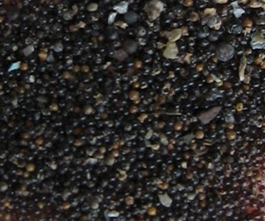
\includegraphics[]{III_A_2.png}
\caption{Une résine échangeuse d'ions}
\label{fig:resine_echangeuse_ions}
\end{figure}

Les résines échangeuses d’ions sont des macromolécules granulaires insolubles. Elles possèdent des radicaux capables de permuter avec certains ions d’une solution de manière réversible. Lors du traitement, la résine se trouve dans un réservoir cylindrique fermé sous pression relié à un filtre et alimenté par un dispositif collecteur du liquide à traiter. Cet ensemble est appelé colonne.

Le processus de traitement consiste à remplacer les ions centraux de complexes polluants par un autre type d’ion qui rendra le nouveau complexe inerte. Il existe 2 types de résines échangeuses d’ions : les résines cathodiques qui remplacent les cations des complexes de la solution (comme l’uranium $\text{U}^{4+}$) par des cations inoffensifs présents sur ces radicaux et les résines anodiques qui permutent des anions de la même manière.
L’échange se fait selon l’équation suivante, de manière réversible sans altération ni solubilisation :
$$R-A^+ + B^+ = R-B^+ + A^+$$
R est le radical de la résine, A l’ion de la résine fixé sur ce radical, et B l’ion à éliminer de la solution.

Le traitement se décompose en plusieurs étapes. Si l’espèce polluante n’est pas sous forme ionique, ou si l’eau contient trop de précipités, une élution est nécessaire. L’eau à traiter est ensuite envoyée grâce à une pompe dans le réservoir jusqu’à saturation de la résine. Ce réservoir est ensuite remplacé et transporté jusqu’au lieu de régénération de la résine, où est opéré le procédé inverse du traitement. L’injection d’une solution régénérante permet de remplacer les ions polluants (comme les ions uranium) par de nouveaux ions inertes. Les résines sont ensuite rincées à faible puis fort débit afin d’éliminer les traces de la solution régénérante. Elles peuvent ensuite être réutilisées pour le processus de traitement de l’eau.

Les réservoirs contenant les résines peuvent être disposés en série, pour augmenter l’efficacité du traitement de l’eau ou bien en parallèle pour augmenter le débit d’eau traité.

Lorsque les colonnes sont en série, le remplacement se fait de manière cyclique : la deuxième colonne prend la place de la première qui est envoyé au site de régénération tandis que la troisième colonne prend la place de la deuxième et ainsi de suite. Une seule nouvelle colonne est ajoutée à la fin de la série. %(Image $III_A_3$)

\begin{figure}[H]
\centering
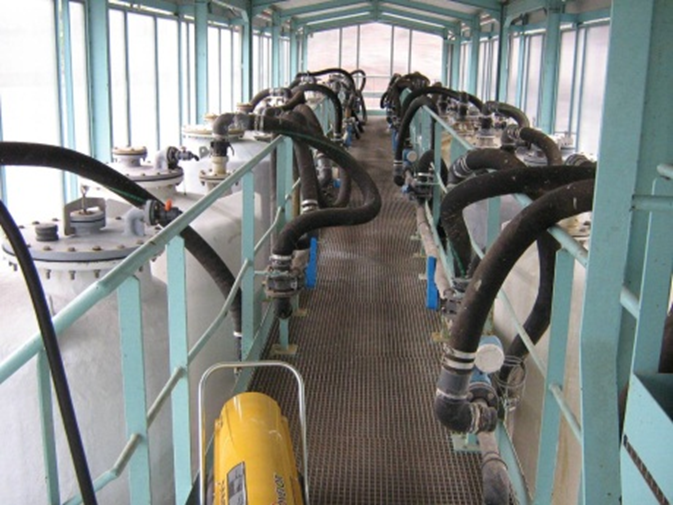
\includegraphics[width=0.9\linewidth]{III_A_3.png}
\caption{Les résines échangeuses d'ions de l'usine de traitement des eaux de Lodève dans l'Hérault (Orano)}
\label{fig:usine_traitement_resines}
\end{figure}

Lors de la régénération des résines, il est possible de traiter la solution régénérante qui ressort du réservoir pour récupérer la substance polluante, soit pour une mise en déchet soit pour réutilisation. Ce processus est notamment très utilisé lors du traitement des eaux pour les mines d’uranium : l’uranium récupéré peut alors être utilisé ou vendu.
Ce type de traitement s’applique principalement à l’uranium dans le cadre des mines et il permet également de traiter des eaux contenant des métaux solubles, des sulfates, des nitrates, des cyanures, des halogénures… Le procédé est plus rarement utilisé pour les polluants organiques.
La majorité des coûts du traitement par résines échangeuses d’ions correspond à l’élution, aux coûts humains, matériels et de transport de la matière polluante.
Un demi équivalent temps plein est nécessaire pour surveiller les différents paramètres de suivi (débits d’eau, concentrations et paramètre de fonctionnements comme la consommation électrique…), pour remplacer les colonnes et nettoyer les filtres.
%(Tableau $III_A_1$)
% \begin{figure}[Ht]
% \centering
% 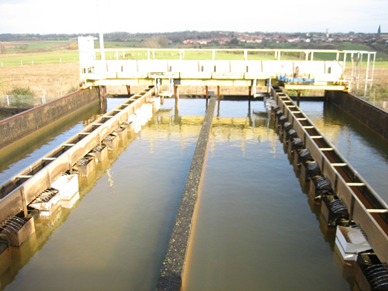
\includegraphics[]{III_A_1.png}
% \caption{Bassin de décantation}
% \label{fig:bassin_decantation}
% \end{figure}


\begin{center}
\begin{tabular}{ |c |c |}
\hline
 Tâche à réaliser & Temps nécessaire pour un fonctionnement hebdomadaire permanent \\ 
 \hline
 Nettoyage des filtres & 8 h / semaine \\ 
 \hline
 Changement des colonnes & 8,5 h / colonne / semaine  \\
 \hline
Analyses & 4h / semaine  \\
 \hline
\end{tabular}
\end{center}

Dans le cas d’une mine d’uranium, la régénération des résines saturées permet de récupérer et revendre l’uranium à un prix avoisinant 80 €/kg.
Le coût du matériel dépend directement du nombre de colonnes nécessaires et donc du débit d’eau à traiter : une colonne coûte 10 500 €.

Le coût du transport correspond notamment aux déplacements des résines vers les lieux de régénération et dépend donc de l’éloignement entre le site de traitement de l’eau et le site de régénération des résines.
L’ensemble des coûts de traitement pour un volume d’eau varie alors entre 0,10 et 0,50 €/$\text{m}^3$.

\paragraph{Traitement par zones humides}

A l’inverse des traitements précédents, les traitements passifs reposent sur des réactions chimiques à l’œuvre naturellement dans l’environnement. Ils ne nécessitent donc pas d’apport d’énergie supplémentaire. 

L’utilisation d’une zone humide (\textit{wetland} en anglais) constitue un moyen de traitement passif des effluents miniers. Le procédé est encore à l’étude et son emploi est encore très marginal en France : parmi les quinze stations de traitement des eaux françaises, une seule en est équipée. Un wetland désigne une étendue d’eau artificielle reproduisant les conditions d’une tourbière dans laquelle transitent des effluents miniers. 

L’abaissement des concentrations en polluants dans l’eau repose sur trois procédés conjoints. D’une part, des bactéries sulfato-réductrices sont nourries par la matière organique présentes dans la tourbe et permettent le maintien du caractère réducteur du milieu. Dans ces conditions, l’uranium tend à précipiter en uraninite insoluble. D’autre part, uranium et radium peuvent être sorbés sur la matière organique ou sur les fractions argileuses présentes dans la tourbe. Enfin, dans le cas des eaux d’exhaure riches en fer, la présence d’une couche d’eau à la surface de la tourbière favorise la précipitation d’oxy-hydroxydes de fer capables de fixer uranium et radium. 

Les coûts d’entretien d’une tourbière sont négligeables. Les seuls coûts significatifs lors de son fonctionnement sont ceux des analyses des eaux en sortie de la zone humide.

%(Image III_A_4)
\begin{figure}[H]
\centering
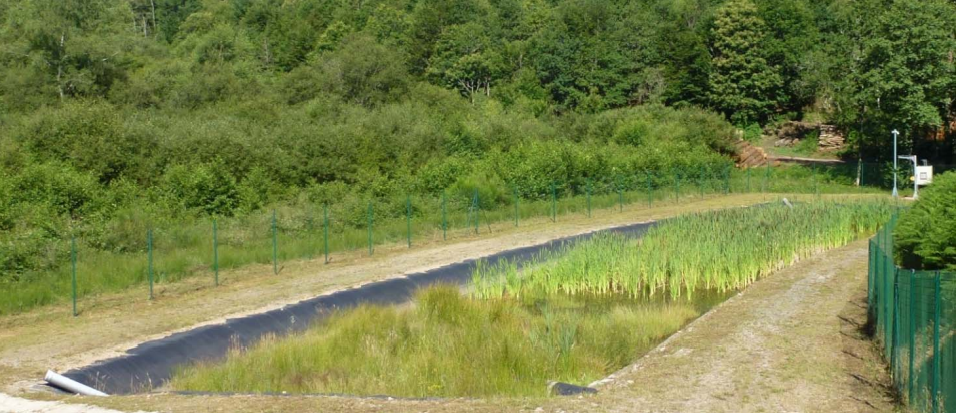
\includegraphics[width=0.8\linewidth]{III_A_4.png}
\caption{Une tourbière}
\label{fig:tourbiere}
\end{figure}


\paragraph{Pas de traitement : prélèvements et analyses}

Il est assez fréquent qu’aucun traitement ne soit nécessaire sur un site minier, lorsque le site est assez isolé ou bien lorsque le traitement qui était nécessaire lors de l’exploitation est devenu inutile (voir III.B). Le coût n’est cependant pas nul, il faut continuer les prélèvements et analyses pour vérifier en permanence que l’eau n’a effectivement pas à être traitée et pouvoir traiter rapidement si un phénomène imprévu présente des dangers (apparition d’un nouveau rejet, effet saisonnier...). Les prélèvements doivent être réalisés au moins une fois par semaine et impliquent donc un coût humain. Il faut également payer les laboratoires responsables des analyses de ces prélèvements.

Le coût est donc, même si aucun traitement n’est mis en place, non négligeable  par rapport au coût total de l’après-mine. Avec ou sans traitement, les prélèvements et analyses réalisés dans l’ensemble de la filière après-mine représentent un investissement de 700 000 à 800 000 € par an.

Il est de même préférable de laisser les infrastructures en place après l'interruption d’un traitement, et de les entretenir régulièrement pour pouvoir recommencer le traitement si nécessaire, et permettre  une meilleure entente avec les associations et les locaux. 


\subsubsection{Comparaison et faisabilité des méthodes de traitement de l'eau}
Les trois méthodes de traitements discutées ci-dessus sont aujourd’hui utilisées en France. Bien qu’elles soient toutes les trois non destructives, elles ne sont pas perçues de la même manière et présentent chacune certains avantages ou aspects contraignants importants à étudier pour savoir quel type de traitement utiliser sur chaque site.


\paragraph{Investissement et mise en place}

Les coûts détaillés à la partie précédente représentent principalement les OPEX (dépenses d’exploitation). Les CAPEX (dépenses d’investissement) représentent également une dépense conséquente qui s'additionne à toute la gestion de l’après-mine. Ce type de dépense doit donc être pris en compte pour choisir un type de traitement plutôt qu’un autre.

Les CAPEX prennent en compte les dépenses liées aux infrastructures et à l’achat du gros matériel non remplacé pendant l’exploitation. Ce coût est équivalent pour ce qui concerne les traitements par précipitation et par zone humide, mais il est 4 à 5 fois plus important pour le traitement par résines échangeuses d’ions.

Il faut cependant également prendre en compte la durée de vie du matériel pour faire un retour sur investissement. Par exemple, si la construction d’un wetland demande un faible investissement, les travaux se réduisant souvent à quelques opérations de terrassement, la tourbe nécessaire à son fonctionnement semble devenir inefficace en quelques années. Or, l’approvisionnement en tourbe a un impact économique et environnemental important, puisque, l’exploitation industrielle de la tourbe française étant strictement réglementée, il peut être nécessaire de l’importer, notamment des pays baltes. 

L’impact environnemental des infrastructures est aussi à prendre en compte. Par exemple, alors que le traitement par précipitation nécessite la construction de nombreux bassins spacieux et pouvant empiéter sur l’environnement, le wetland s’insère dans le paysage, accueillant la végétation et permettant le développement d’une faune spécifique.

\paragraph{Exploitation et maintenance}

Les méthodes de traitement présentent chacune des avantages et inconvénients relatifs à leur exploitation. D’une part, leurs caractéristiques techniques ne leur permettent pas de prendre en charge les mêmes débits d’effluents. Le traitement par précipitation et coagulation-floculation-décantation est le plus productif, avec environ 200 $\text{m}^3$ traités par heure, mais aussi le plus flexible, avec une bonne capacité d’adaptation aux variations saisonnières du volume d’effluent entrant. 
Le traitement par résines échangeuses d’ions permet le traitement d’environ 100 $\text{m}^3$ d’effluent par heure et présente une bonne adaptabilité au débit grâce à la possibilité de placer les bouteilles en série ou en parallèle. Au contraire, le wetland ne traite que de très faibles débits, de l’ordre du $\text{m}^3$ par heure.

Le traitement par résines échangeuses d’ions est le traitement le plus efficace pour abattre la concentration en uranium de l’eau avec un rendement pouvant atteindre 95\% ou même 98\% lorsque les colonnes sont disposées en série.  Tout comme le procédé de précipitation, qui permet d’atteindre dans de bonnes conditions des rendements de 90\%, il est en mesure d’éliminer une large gamme de polluants grâce au recours à différentes résines. L’efficacité de ces deux traitements est en outre sensible aux caractéristiques chimiques de l’effluent, telles que son pH ou la présence de certains éléments. Pour le traitement par résines, la présence de précipités peut très fortement nuire au traitement. Un prétraitement, l’élution, est alors nécessaire et représente la majorité des coûts du traitement par résines. Le wetland est de nouveau la solution la moins efficace, l’abattage des concentrations en uranium et radium étant de l’ordre de 50 à 70\%.

Le traitement par résines met en jeu des réactions rapides qui permettent, sous réserve de bonnes conditions chimiques, un traitement rapide des eaux. A l’inverse, le traitement par précipitation repose sur une longue phase de décantation pouvant durer plusieurs jours. Les deux solutions de traitement actif présentent également des coûts importants en maintenance (transport des résines, manutention des colonnes, nettoyage préventif des cuves) et en réactifs tandis que l’utilisation du wetland ne requiert pas la présence permanente d’un opérateur. Les seuls coûts associés à son fonctionnement sont les coûts des analyses de l’eau en sortie.  Néanmoins, la durée d’efficacité du wetland semble courte : des données relevées en 2020 au bassin pilote de la mine d’Henriette ouvert en 2014 montrent que l’abattage des concentrations en polluants est moins important après cinq ans d’activité. 

En termes de coûts, les traitements par zones humides et par précipitation sont plus avantageux que celui par résine car l’investissement et l’élution sont trop coûteux, même en prenant en compte les éventuelles ventes après régénération de la résine.
%(Tableau III.A.2)


\begin{figure}[H]
    \centering    
    \begin{tabular}{ |c |c |}
        \hline
         \textbf{Type de traitement} & \textbf{Coût d’exploitation en €/m$^3$} \\ 
         \hline
         Précipitations & 0,20 à 0,50 \\ 
         \hline
         Résines échangeuses d’ions & 0,10 à 0,50 (avec revente du polluant)  \\
         \hline
        Zones humides & Négligeable  \\
         \hline
    \end{tabular}
    \caption{Coût d'exploitation des différents traitements \cite{schick_les_2020}}
\label{tab:cout_exploitation_traitements}
\end{figure}

L’un des principaux enjeux de l’après-mine est de diminuer ces coûts car le traitement par résine est très avantageux lorsque le polluant peut être récupéré.

\paragraph{Gestion des déchets }

Les traitements produisent des déchets sous différentes formes qu’il est nécessaire de stocker où d’évacuer en respectant les normes et les sociétés locales.

Le traitement par zone humide engendre des tourbes saturées au bout de quelques années. La question de la gestion de cette matière organique chargée est encore à l’étude. En outre, l’utilisation d’un wetland peut entraîner le relargage des métaux fixés dans l’environnement avoisinant.
De même, le traitement par précipitation donne naissance à d’importants volumes de boues qui impliquent de nouveaux coûts de traitement ou de déshydratation. Il peut également augmenter les concentrations en sulfates dans l’eau. 

Au contraire, le traitement par résines échangeuses d’ions est très bien perçu par les associations car il permet de retirer définitivement un certain type de polluant du site minier. C’est notamment le cas pour les mines d’uranium : les associations qui se focalisent sur les dangers liés à l’uranium sont satisfaites par l’exportation de ce dernier vers d’autres lieux ou il va être traité puis revendu lors de la régénération des résines.

Cependant ce type de traitement provoque la création de nouveaux déchets, à l’extérieur du site minier, lorsque le polluant ne peut pas être réutilisé après avoir été récupéré lors de la régénération des résines. Le problème est donc dans ce cas le même que la gestion des déchets liés aux traitements par zones humides et précipitations.

Le traitement de l’eau par résine échangeuse d’ion est alors plus avantageux que les autres principalement dans le cas où le polluant peut être récupéré après régénération de la résine: le coût est diminué grâce à la revente et le processus ne produit presque pas de déchets.

Ne pas traiter une eau dont les teneurs en polluants sont en adéquation avec les normes en vigueur est aussi une solution pertinente sur les plans environnementaux et économiques, son coût se réduisant aux frais de contrôle et d’analyse des eaux. Cette solution pourrait également être pertinente dans le cas où l’évacuation de l’eau vers un cours d’eau met en jeu des dilutions importantes. Néanmoins, du fait de l’exacerbation de la dangerosité de l’uranium dans l’opinion collective, un traitement, même s’il est plus susceptible de dégrader la qualité de l’eau que de l’améliorer, est souvent préféré par les populations locales. De même, l’interruption d’un traitement des eaux est susceptible d’être mal accueillie par les riverains.

\subsubsection{Présentation des situations des autres pays}
\paragraph{Situation générale de mines d’uranium de chaque pays}
\paragraph{Les méthodes de traitement préférées par pays}

\subsection{Les traitements sont-ils toujours nécessaires ? Étude de cas du site de la Ribière}
\subsubsection{Présentation du site de La Ribière}
L’étude du traitement des eaux d’exhaure d’une mine nécessitait de se baser sur un exemple concret, et c’est pour cette raison que nous nous sommes penchés sur le site de la Ribière. 

Situé sur la commune de Domeyrot dans la Creuse, ce site a été exploité de 1959 à 1984 par la compagnie TCMF (\emph{Total Compagnie Minière France}), qui en a extrait 142,9 tonnes d’uranium sur l’ensemble de la durée d’exploitation. Pour récupérer cette quantité d’uranium, il a fallu extraire 628 kt d’une mine à ciel ouvert (MCO) d’une superficie de 17 472 m². Il n’y a pas de travaux miniers souterrains à la Ribière.

Le traitement du minerai brut extrait a conduit, d’une part à l’uranium, et d’autre part à un volume important de résidus et de stériles miniers. Ainsi, une partie de ces résidus a été stockée sur le site, dans l’emplacement correspondant à l'ancienne mine à ciel ouvert, et pour une masse totale de 192 000 tonnes.

Ces résidus, placés en grande partie dans l’ancienne MCO, ont été traités de manière statique, par lixiviation \textit{in situ} entre 1982 et 1985. Il s'agissait d’un minerai pauvre en uranium, avec une concentration de l’ordre de 350 ppm. 

Puis, une fois cette phase de dépôt effectuée, le site est entré en phase de réaménagement entre 1991 et 1992, par son recouvrement avec une couche de stériles et de terre épaisse de 4 mètres et sa végétalisation (partielle). La surface est recouverte d’herbe étant donné que l’on ne peut pas laisser un système racinaire développé s’implanter, car cela favoriserait une infiltration trop importante d’eau.

Le site constitue un bassin versant d’altitude maximale 405 mètres, avec le ruisseau Le Verraux qui le longe dans sa partie inférieure, à un altitude de 348 mètres.

Désormais géré par Orano Mining, le site de la Ribière a été équipé d'appareils de mesure et de surveillance, notamment pour ce qui est de l’eau qui traverse le site. Ainsi sont répartis sur les 14 ha 4 points de surface pour la surveillance environnementale, et 9 piézomètres qui s’enfoncent dans le sol afin d’en avoir une vision détaillée, et notamment le profil géologique et hydrologique de la zone.

Selon Orano Mining, le site, qui ne dispose pas de station de traitement des eaux, respecte les normes environnementales en vigueur en termes de qualité des eaux à l’exutoire. La concentration en uranium mesurée est de $7,6 \cdot 10^{-6} $ mol/L et la dose mesurée est de $1,37$ Bq/L pour le $^{226}$Ra.

Nous nous proposons donc de mettre en œuvre deux modèles du site, hydrologique et géochimique, afin de confirmer ces mesures et d’obtenir une prévision de long terme quant au respect de ces normes. 

\subsubsection{Modèle géochimique et 1D}
\paragraph{Modélisation}

Nous avons réalisé, dans le cadre de l’étude de cas du site de La Ribière, un modèle géochimique des résidus, dans le but de modéliser ce qui se passe sur le site, en accord avec les mesures piézométriques, et comprendre les mécanismes de la mobilité de l’uranium. Nous avons également utilisé le modèle pour effectuer des prévisions à long terme.
Pour réaliser le modèle, nous nous sommes servi des mesures effectuées dans les deux faciès, qui visaient à reconnaître les minéraux présents et la concentration des oxydes. (Annexe image 1 et 2) Nous avons sélectionné les oxydes principaux et ensuite déduis les minéraux qui pouvaient les contenir, pour arriver à une liste de 9 minéraux représentatifs de chaque faciès. Les concentrations de chaque minéral a ensuite été calculée en kilogramme par litre d’eau à l’aide des concentrations en oxydes. 
	
	(tableau à mettre) + (voir annexe)
	
Nous avons ainsi pu écrire un code Hytec pour calculer l’équilibre initial des deux faciès. Nous avons comparé les valeurs de pH, de concentration aqueuse en $UO_2^{2+}$, et en $SO_4^{2-}$ avec les mesures du piézomètre 3. Notre modèle correspondant bien à la réalité, nous avons gardé la géochimie précédemment calculée. Nous avons choisi de ne pas prendre en compte le radium.
	
	(deuxième tableau)
	
Pour étudier la mobilité de l’uranium, nous avons utilisé notre modèle géochimique pour créer une colonne 1D avec au début 30 mètre de résidus (faciès sableux) puis 170 mètres de granite. Nous avons ensuite ajouté un flux d’eau partant de la gauche pour s’écouler vers la droite. Les paramètres physiques correspondent à ceux du site de La Ribière. Pour la vitesse de l’écoulement, nous avons utilisé la hauteur de charge, la porosité et la perméabilité des différents faciès traversés. Pour obtenir un modèle le plus réaliste possible, nous avons choisi d’équilibrer l’eau injectée dans les résidus avec un granite basique, comme celui placé après le bloc de résidus. (code en annexe)


\begin{figure}[H]
    \centering
    \includegraphics[width=0.9\linewidth]{III_B_1.png}
    \caption{Modélisation 1D des blocs de résidus (en rouge) et de granite (en gris)}
    \label{fig:modele_bloc}
\end{figure}

Enfin, nous avons réalisé différentes simulations sur 100 ans pour étudier la mobilité de l’uranium et les facteurs l’influençant et nous les avons visualisées à l’aide du logiciel ParaView.


\paragraph{Résultats du modèle géochimique }
\paragraph{Etude du faciès sable}

La première simulation réalisée vise à étudier la mobilité de l’uranium dans les conditions du site. Le pH de l’eau injectée est fixé à $6,1$, pH mesurer au niveau du piézomètre 2, juste avant la zone de résidus. Dans un premier temps, nous avons regardé l’effet de l’écoulement d’eau sur les résidus, et en particulier sur l’autunite, de formule $Ca(UO_2)_2(PO_4)_2(H_2O)_3$.

\begin{figure}[H]
    \centering
    \includegraphics[width=0.9\linewidth]{III_B_1.png}
    \caption{Modélisation 1D des blocs de résidus (en rouge) et de granite (en gris)}
    \label{fig:modele_bloc}
\end{figure}

On peut alors remarque que la quantité d’autunite est dissoute au cours du temps. Le phénomène en jeu ici est la dissolution de l’autunite. Un équilibre chimique va s’établir entre l’eau et les résidus. La concentration aqueuse en $UO_2^{2+}$ de l’eau injectée est nulle, ainsi l’autunite va se dissoudre pour que le système soit à l’équilibre. Cependant, on remarque que la concentration aqueuse en $UO_2^{2+}$ au niveau des résidus chute assez rapidement.

(image 3)

La concentration à l’équilibre initiale est environ $1 \mu mol/L$, puis en seulement 5 ans, elle est divisée par 10, pour finalement atteindre moins de $10^{-2} \mu mol/L$. L’uranium ne reste pas en solution. Il est en fait fixé sur la Montmorillonite et la Ferrihydrite grâce au phénomène de sorption.

(image 4)

La sorption est un phénomène d’échange cationique sur des sites libres en surface de minéraux, notamment sur les argiles. Son efficacité dépend donc de la surface spécifique des minéraux impliqués dans la sorption (typiquement $600 m^2/g$ pour les argiles) et de la capacité de fixation, qui est de l’ordre de $1 \mu mol/m^2$ (soit $6 \times 10^{-4} mol/g$ pour les argiles). Cependant, $UO_2^{2+}$ n’est pas le seul cation présent en solution pouvant être fixé. Les cations $Ca^{2+}$, $K^{+}$, $H^{+}$ et $Mg^{2+}$ peuvent également se fixer sur la Montmorillonite. Cependant, pour le pH étudié, seul $Ca^{2+}$ se fixe au cours du temps. Les trois autres ont plutôt tendance à être libérés, ils n’empêchent donc pas la sorption de l’uranium. \emph{(annexe images 1 à 4)}
Dans un deuxième temps, nous avons regardé les caractéristiques physico-chimiques de l’eau rejetée dans la rivière : le pH, la concentration aqueuse en $UO_2^{2+}$, en $Fe^{3+}$ et en $Ba^{2+}$.

\begin{figure}[H]
    \centering
    \begin{minipage}{0.5\textwidth}
        \centering
        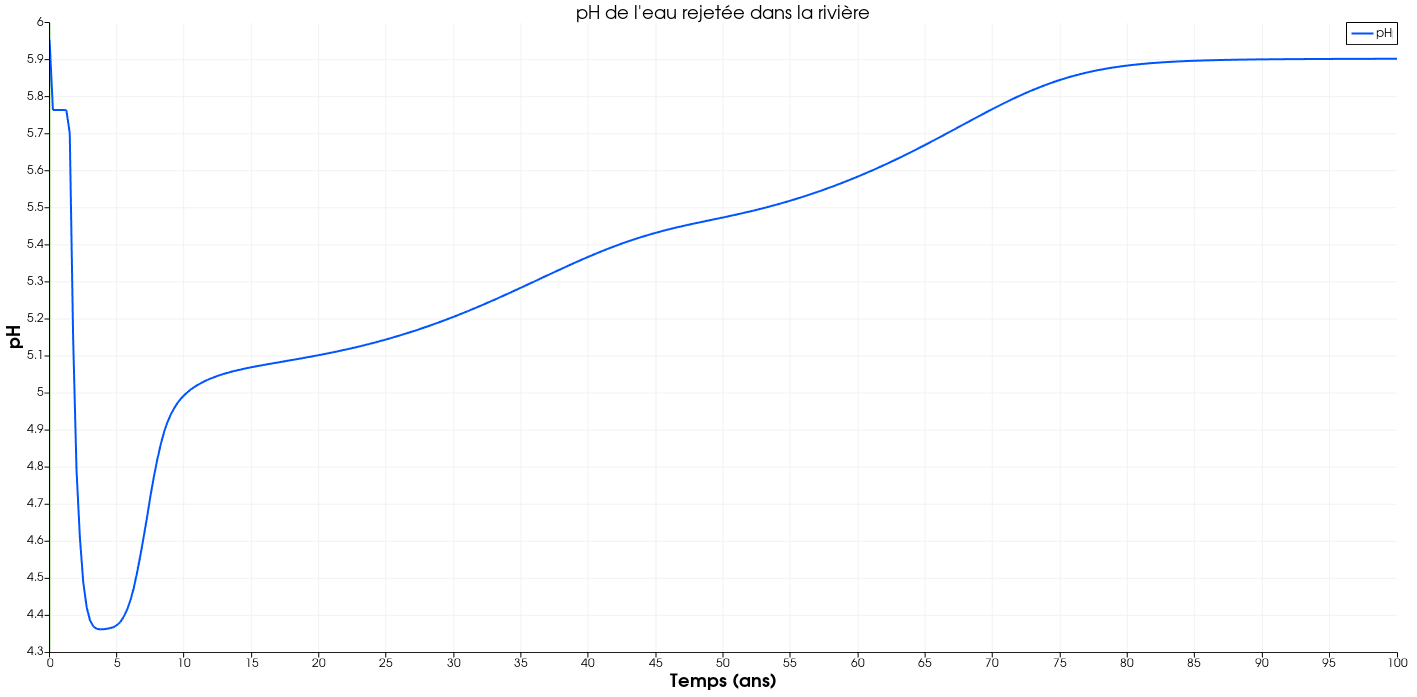
\includegraphics[width=0.9\textwidth]{III_B_2_5.png} 
        \caption{}
        \label{fig:pH_sable_Base}
    \end{minipage}\hfill
    \begin{minipage}{0.5\textwidth}
        \centering
        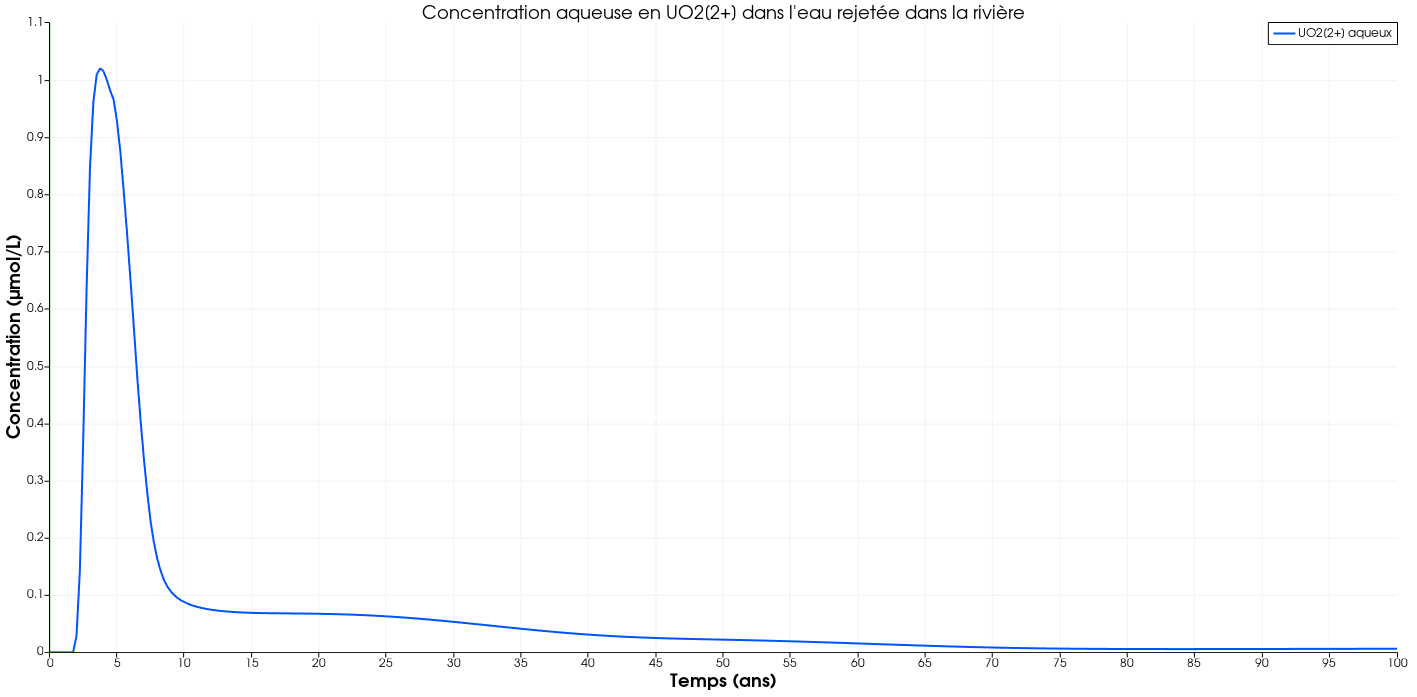
\includegraphics[width=0.9\textwidth]{III_B_2_6.png} 
        \caption{}
        \label{fig:UO2_riviere_sable_base}
    \end{minipage}
\end{figure}

\begin{figure}[H]
    \centering
    \begin{minipage}{0.5\textwidth}
        \centering
        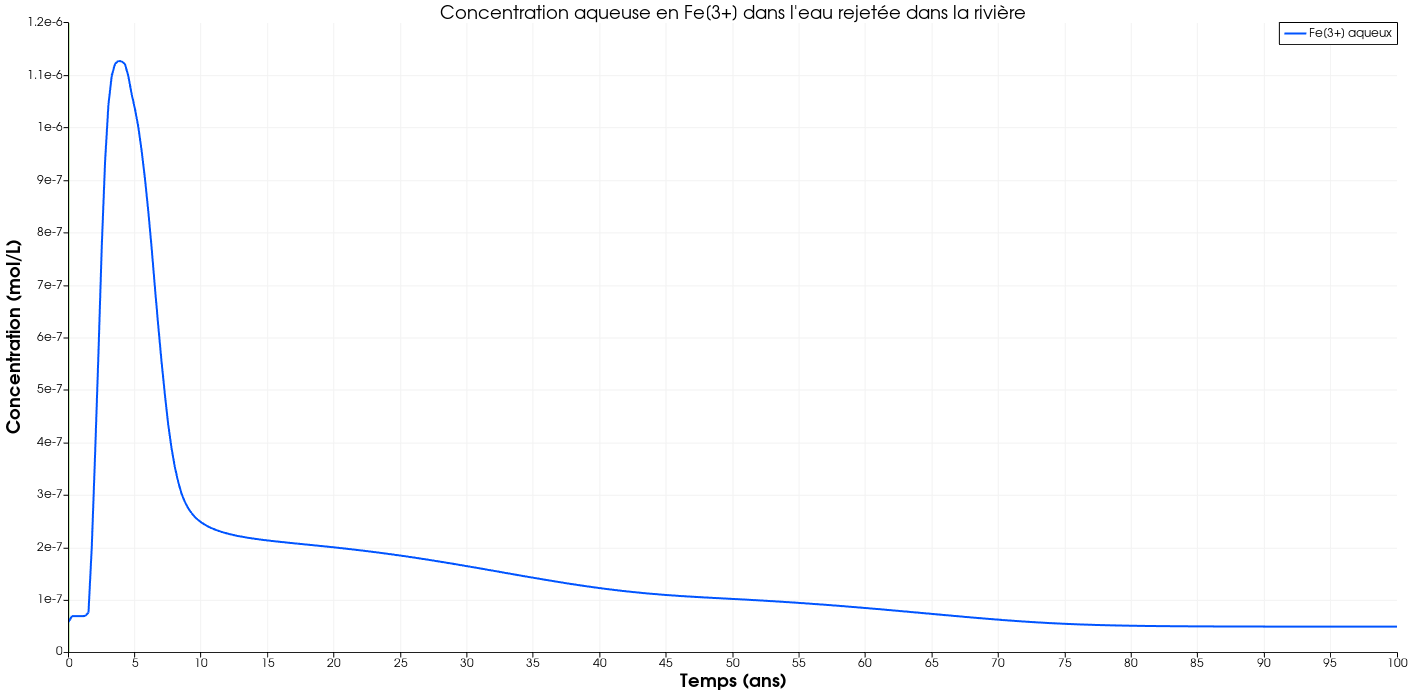
\includegraphics[width=0.9\textwidth]{III_B_2_7.png} 
        \caption{}
        \label{fig:Fe_riviere_sable_Base}
    \end{minipage}\hfill
    \begin{minipage}{0.5\textwidth}
        \centering
        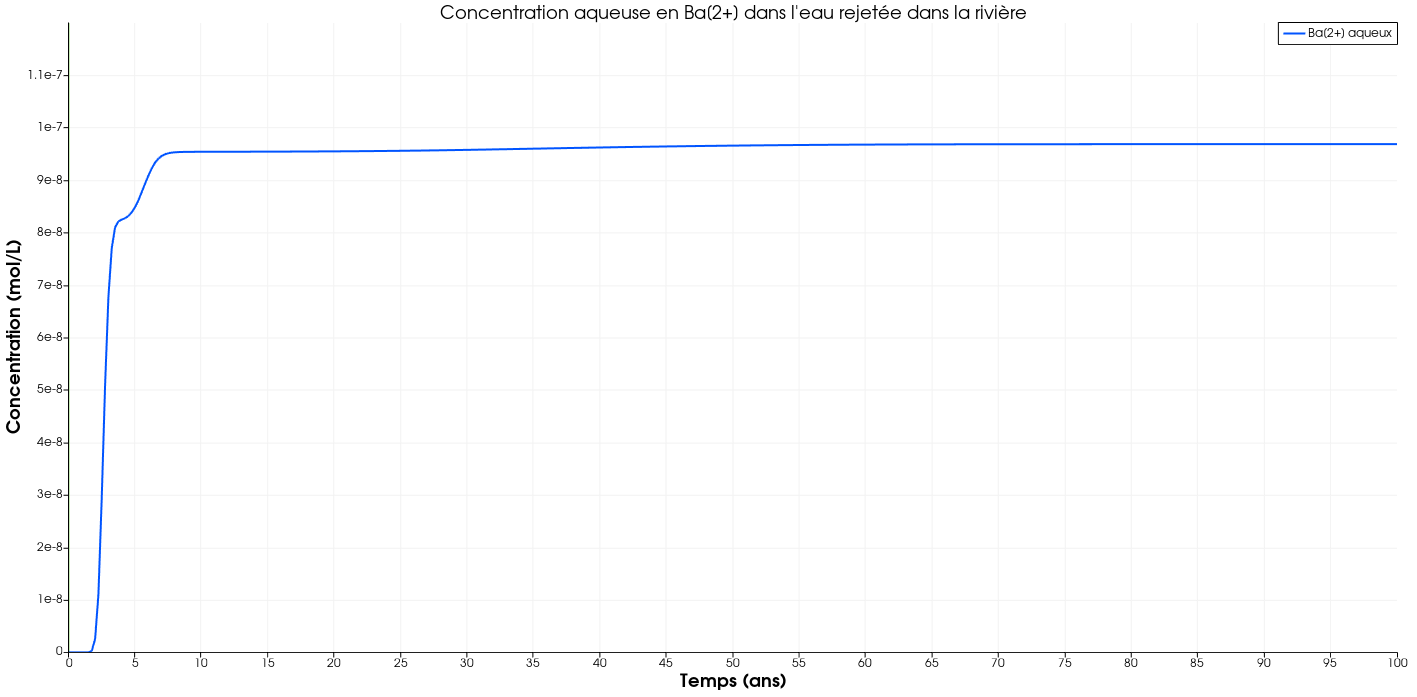
\includegraphics[width=0.9\textwidth]{III_B_2_8.png} 
        \caption{}
        \label{fig:Ba_riviere_sable_base}
    \end{minipage}
\end{figure}

On remarque alors pour l’uranium un pic à $1 \mu mol/L$ correspondant au déplacement des ions en solution à l’équilibre initial, puis un établissement de la concentration inférieur à $0,1 \mu mol/L$. Cependant, la concentration augmente doucement à partir de 80 ans. En effet, les sites de sorption disponibles sont de moins en moins nombreux et donc les cations d’oxyde d’uranium sont de moins en moins fixés dans les résidus. Mais le phénomène reste faible. La concentration en baryum est négligeable et celle en fer ne dépasse pas les $70 \times 10^{-3} mg/L$. la norme de potabilité pour le fer est placée à $0,2 mg/L$, il n’y a donc aucun problème pour le fer.


\paragraph{Influence du pH sur la mobilité de l'uranium}

Pour étudier l’influence du pH sur la mobilité de l’uranium, nous avons choisi de changer le pH de l’eau injectée en entrée du modèle. Nous avons fait les simulations pour deux autres pH d’entrée : $4$ et $8$. Les résultats pour les trois pH sont superposés sur les mêmes courbes.

\begin{figure}[H]
    \centering
    \begin{minipage}{0.5\textwidth}
        \centering
        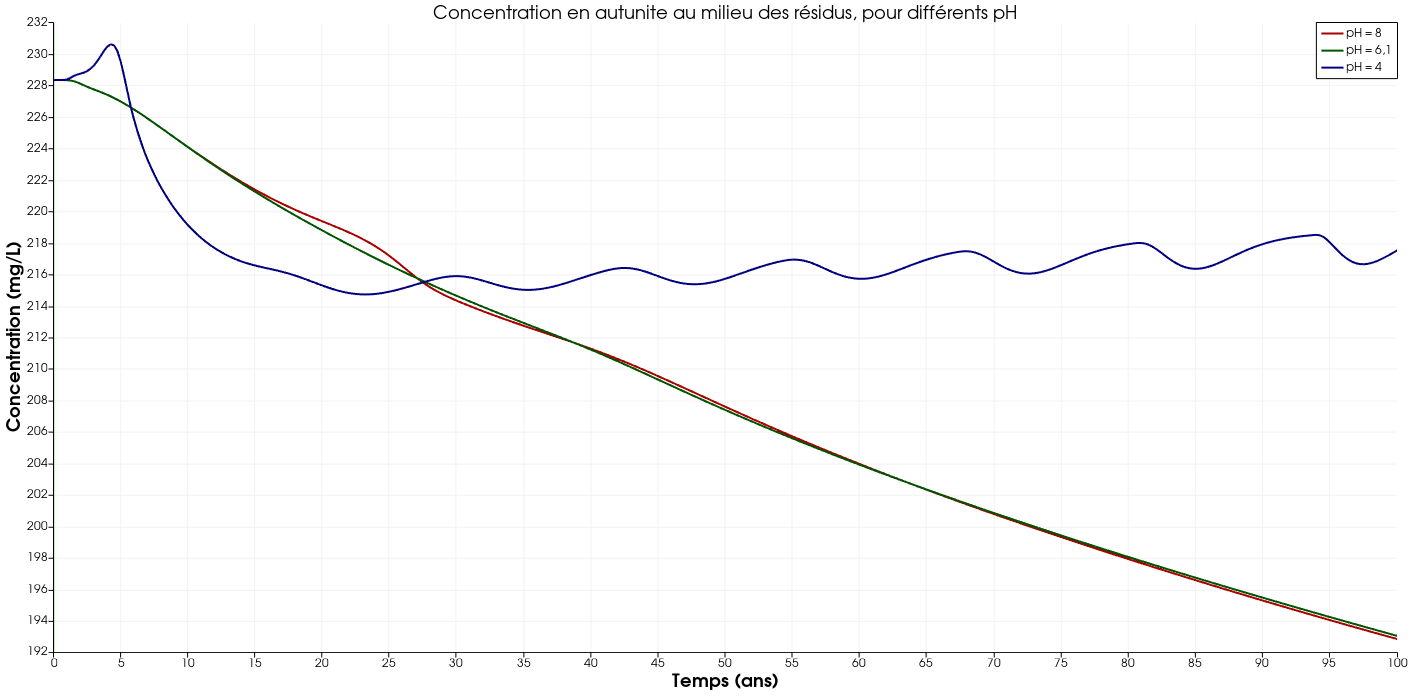
\includegraphics[width=0.9\textwidth]{III_B_2_9.png} 
        \caption{}
        \label{fig:autunite_residus_comparaison}
    \end{minipage}\hfill
    \begin{minipage}{0.5\textwidth}
        \centering
        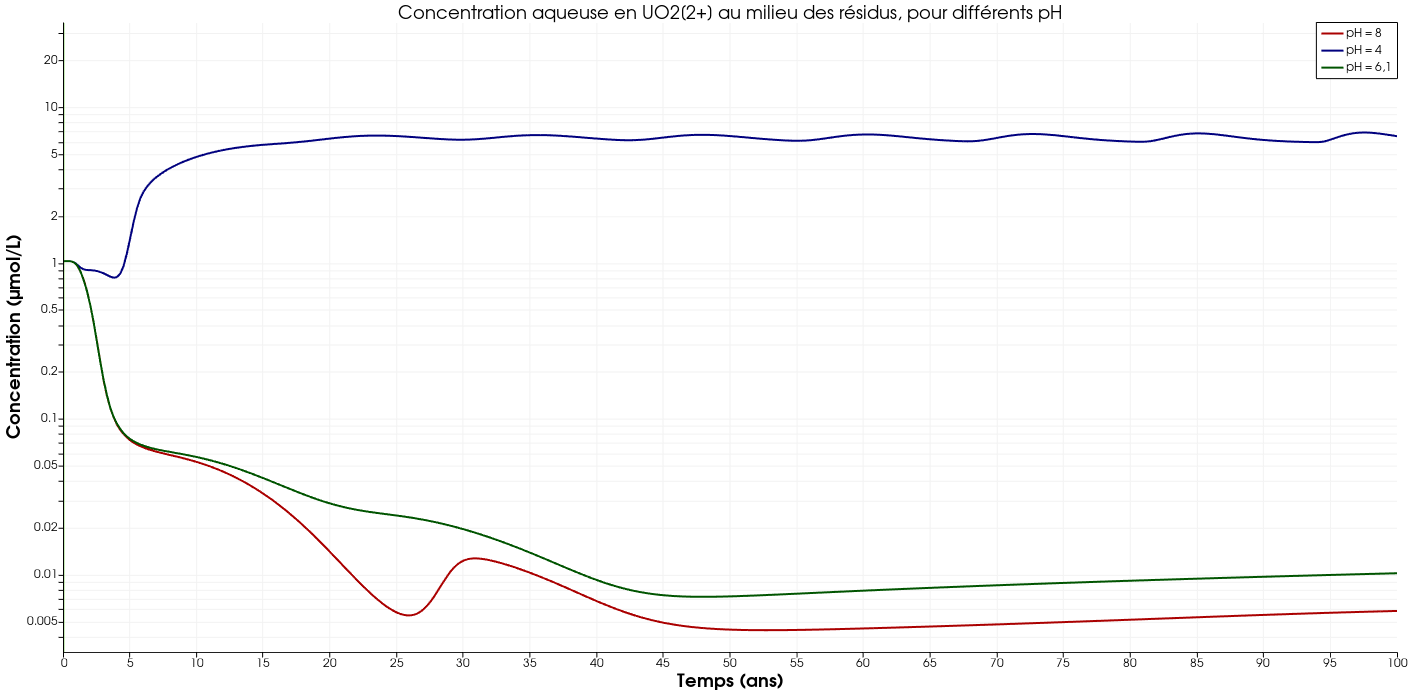
\includegraphics[width=0.9\textwidth]{III_B_2_10.png} 
        \caption{}
        \label{fig:UO2_residus_comparaison}
    \end{minipage}
\end{figure}

\begin{figure}[H]
    \centering
    \begin{minipage}{0.5\textwidth}
        \centering
        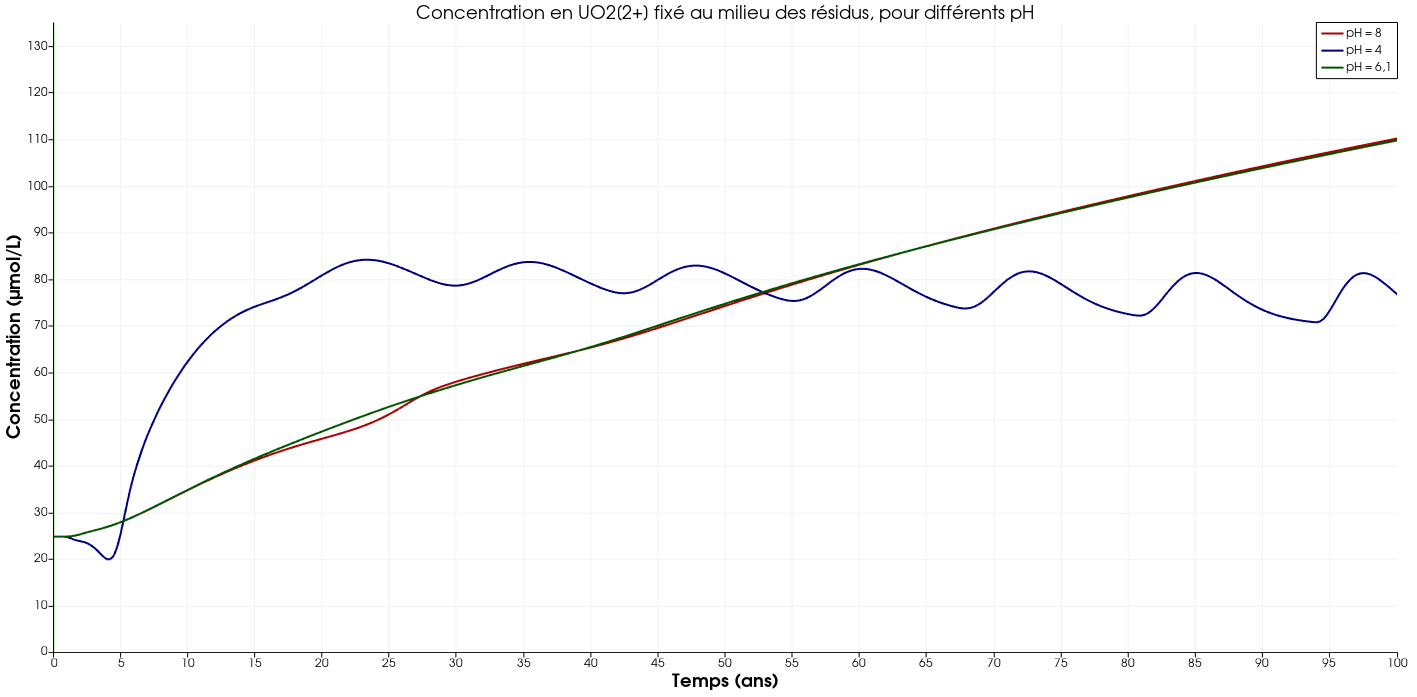
\includegraphics[width=0.9\textwidth]{III_B_2_11.png} 
        \caption{}
        \label{fig:UO2_fixe_rsidus_comparaison}
    \end{minipage}\hfill
    \begin{minipage}{0.5\textwidth}
        \centering
        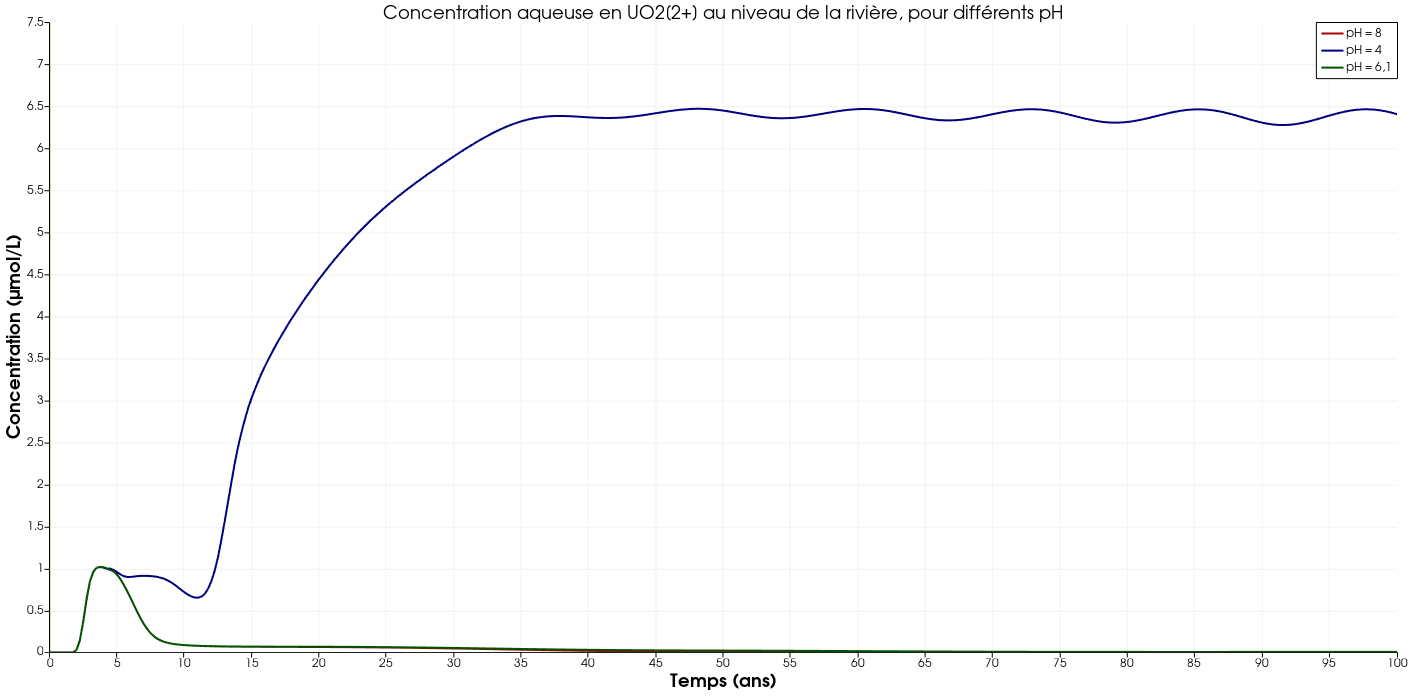
\includegraphics[width=0.9\textwidth]{III_B_2_12.png} 
        \caption{}
        \label{fig:UO2_riviere_comparaison}
    \end{minipage}
\end{figure}


Lorsque que le pH devient très acide, la concentration aqueuse en $UO_2^{2+}$ au niveau des résidus augmente et la concentration d’ions fixés diminue par rapport aux pH neutre et basique. La dissolution de l’autunite est moins régulière : elle se fait plus par paliers, en commençant par le premier endroit en contact avec le pH acide. Il y a donc plus d’ion $UO_2^{2+}$ en solution et ils sont beaucoup moins fixés. On peut donc voir qu’une concentration bien plus importante atteint la rivière (presque 100 fois plus que pour un pH neutre ou basique). De plus, d’autre polluant comme le fer et le baryum sont également plus présent.

\begin{figure}[H]
    \centering
    \begin{minipage}{0.5\textwidth}
        \centering
        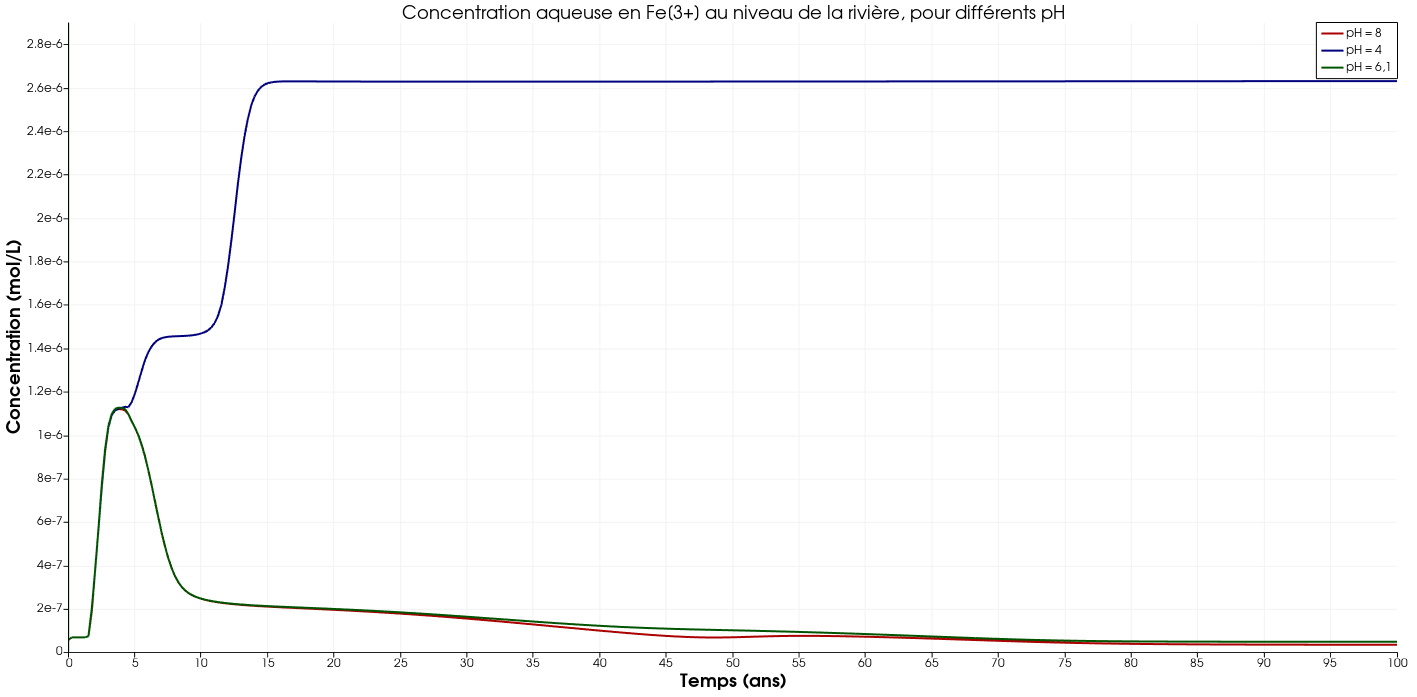
\includegraphics[width=0.9\textwidth]{III_B_2_13.png} 
        \caption{}
        \label{fig:Fe_riviere_comparaison}
    \end{minipage}\hfill
    \begin{minipage}{0.5\textwidth}
        \centering
        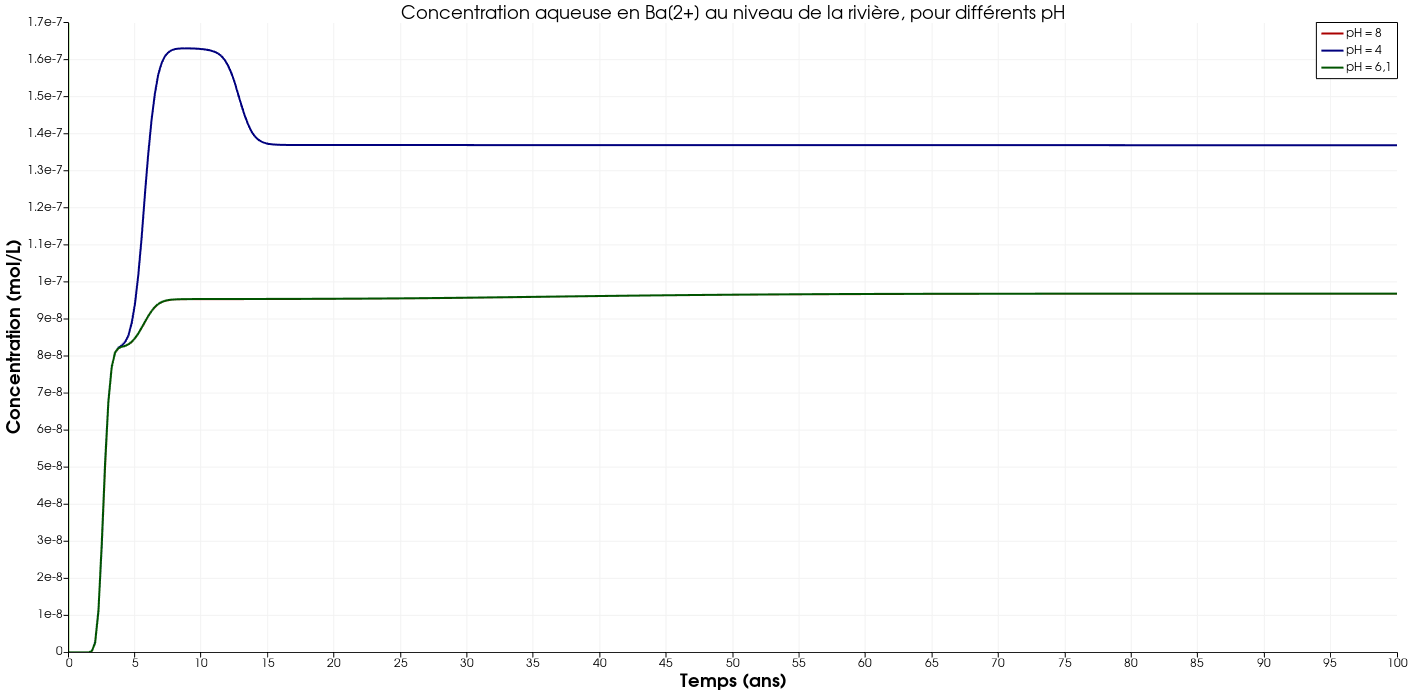
\includegraphics[width=0.9\textwidth]{III_B_2_14.png} 
        \caption{}
        \label{fig:Ba_rivier_comparaison}
    \end{minipage}
\end{figure}

Pour comprendre pourquoi l’uranium était moins fixé, nous avons regardé les concentrations des autres cations fixés sur la montmorillonite.

(images 17)
\begin{figure}[H]
    \centering
    \begin{minipage}{0.5\textwidth}
        \centering
        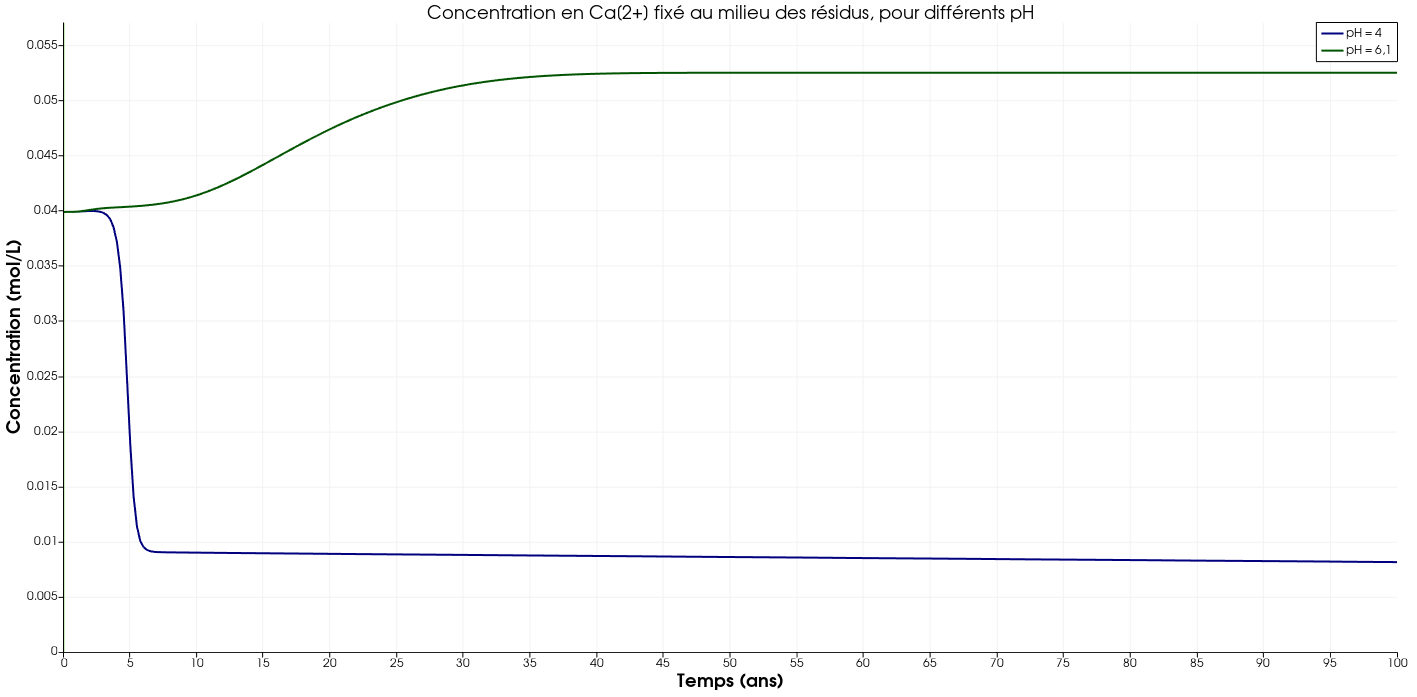
\includegraphics[width=0.9\textwidth]{III_B_2_15.png} 
        \caption{}
        \label{fig:Ca_residus_comparaison}
    \end{minipage}\hfill
    \begin{minipage}{0.5\textwidth}
        \centering
        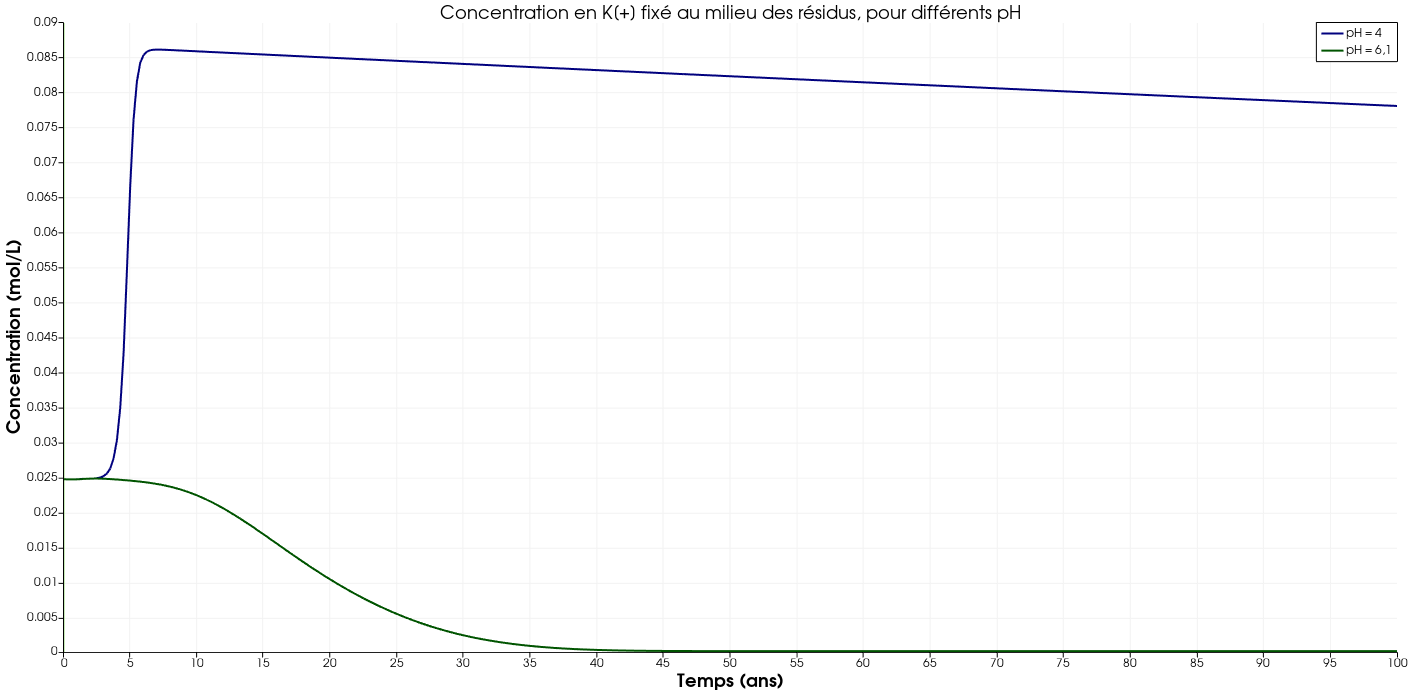
\includegraphics[width=0.9\textwidth]{III_B_2_16.png} 
        \caption{}
        \label{fig:K_residus_comparaison}
    \end{minipage}
\end{figure}


Hormis le calcium, les autres cations sont plus fixés avec un pH bas. Un pH plus élevé ne change presque rien. Les sites de fixation sont en fait préférentiellement utilisés par les cations $Mg^{2+}$ et $K^{+}$, empêchant alors l’uranium de se fixer.
En conclusion, le pH influence beaucoup la mobilité de l’uranium. Un pH plus élevé (basique) ne change presque rien à la sorption de l’uranium et donc à la concentration aqueuse en $UO_2^{2+}$ dans l’eau rejetée dans la rivière par rapport au pH initial de $6,1$. Cependant, lorsque le pH devient acide, les cations d’uranium sont beaucoup moins fixés, car remplacés par du magnésium et du potassium. Il y a donc une concentration en $UO_2^{2+}$ beaucoup plus élevée en sortie du modèle. Le contrôle du pH en amont des résidus est donc primordial pour le site.

\paragraph{Etude d'une possibilité de sorption sur des hydroxydes d'aluminium précipités}
Avec le modèle, nous avons essayé de mettre en place un traitement de l’eau par sorption sur des hydroxyde d’aluminium. Nous avons donc injecté des ions $Al^{3+}$ en solution en entrée du modèle. Cependant, la précipitation de $Al(OH)_3$ consomme des ions $OH^{-}$ et donc diminue le pH (il est alors autour de $4,5$). On observe donc une augmentation d’ions $UO_2^{2+}$ en solution. De plus, l’hydroxyde d’aluminium ne précipite que à l’entrée du modèle (dans les deux premières mailles).

\begin{figure}[H]
    \centering
    \begin{minipage}{0.5\textwidth}
        \centering
        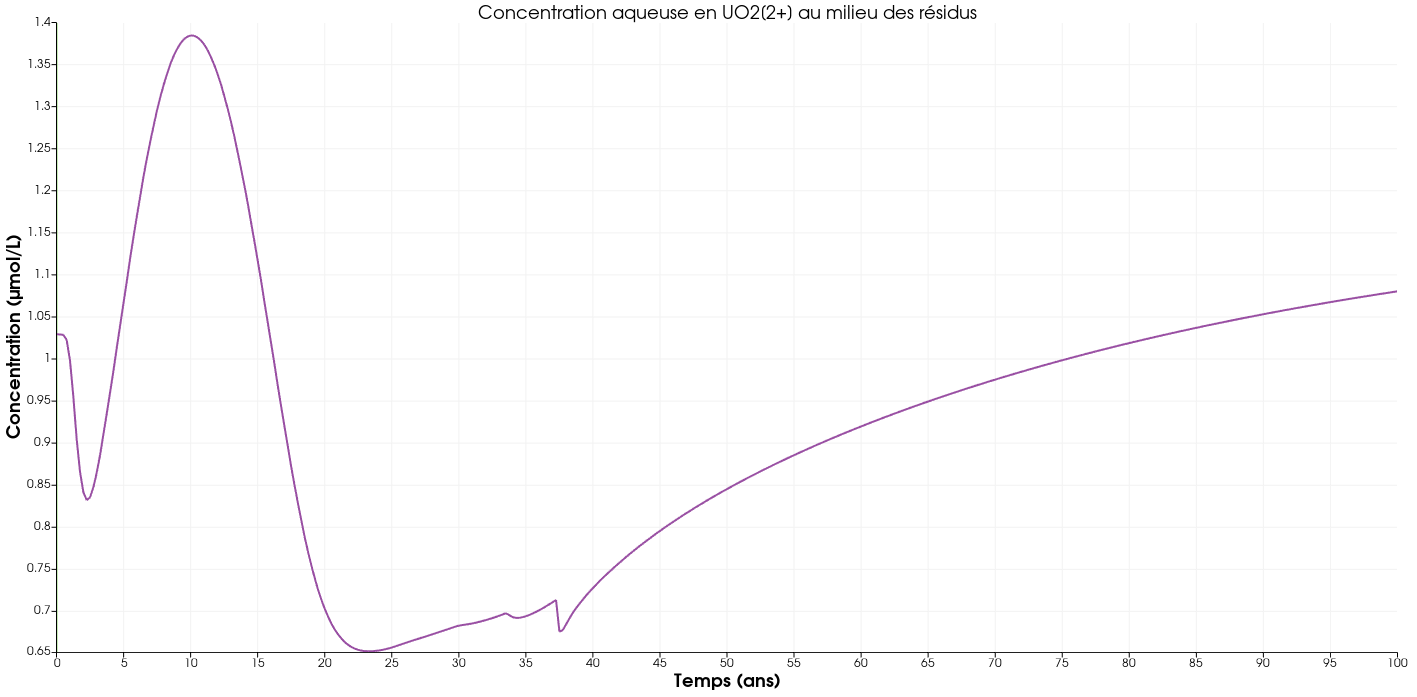
\includegraphics[width=0.9\textwidth]{III_B_2_18.png} 
        \caption{}
        \label{fig:UO2_residus_Al}
    \end{minipage}\hfill
    \begin{minipage}{0.5\textwidth}
        \centering
        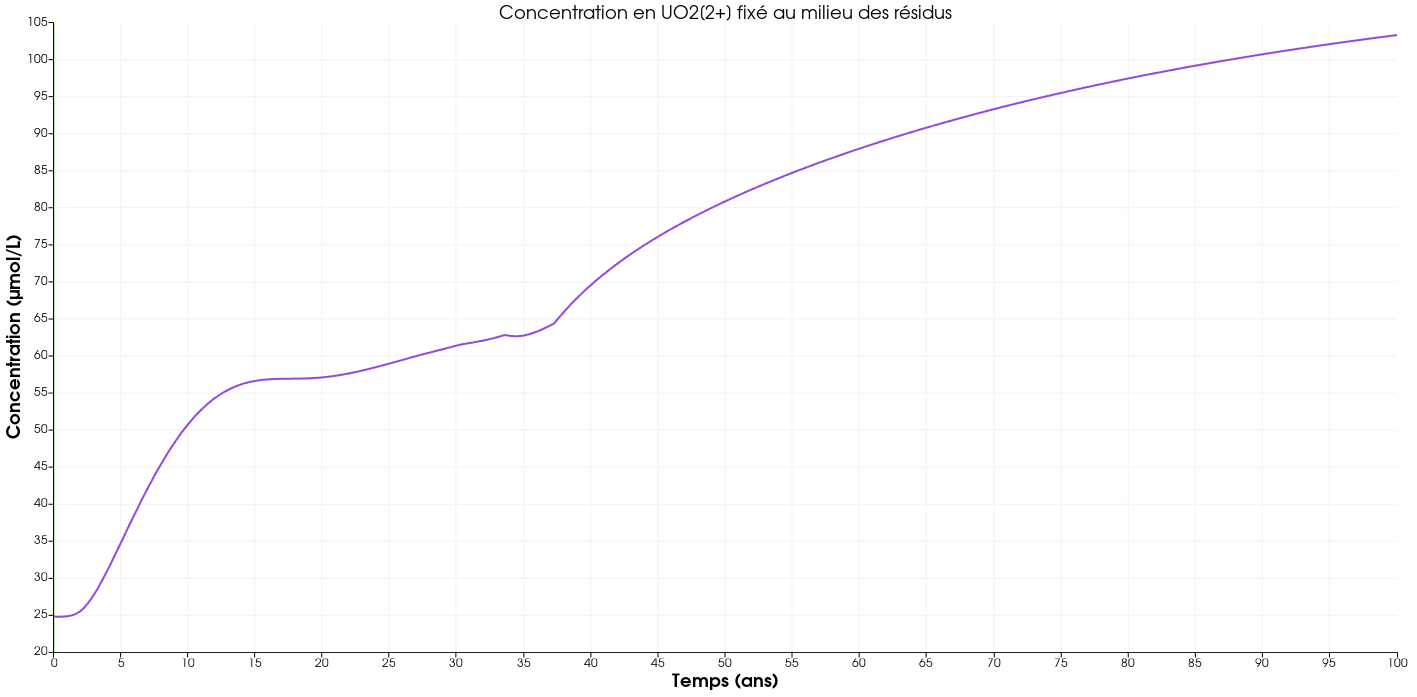
\includegraphics[width=0.9\textwidth]{III_B_2_19.png} 
        \caption{}
        \label{fig:UO2_fixe_residus_Al}
    \end{minipage}
\end{figure}

\begin{figure}[H]
    \centering
    \begin{minipage}{0.5\textwidth}
        \centering
        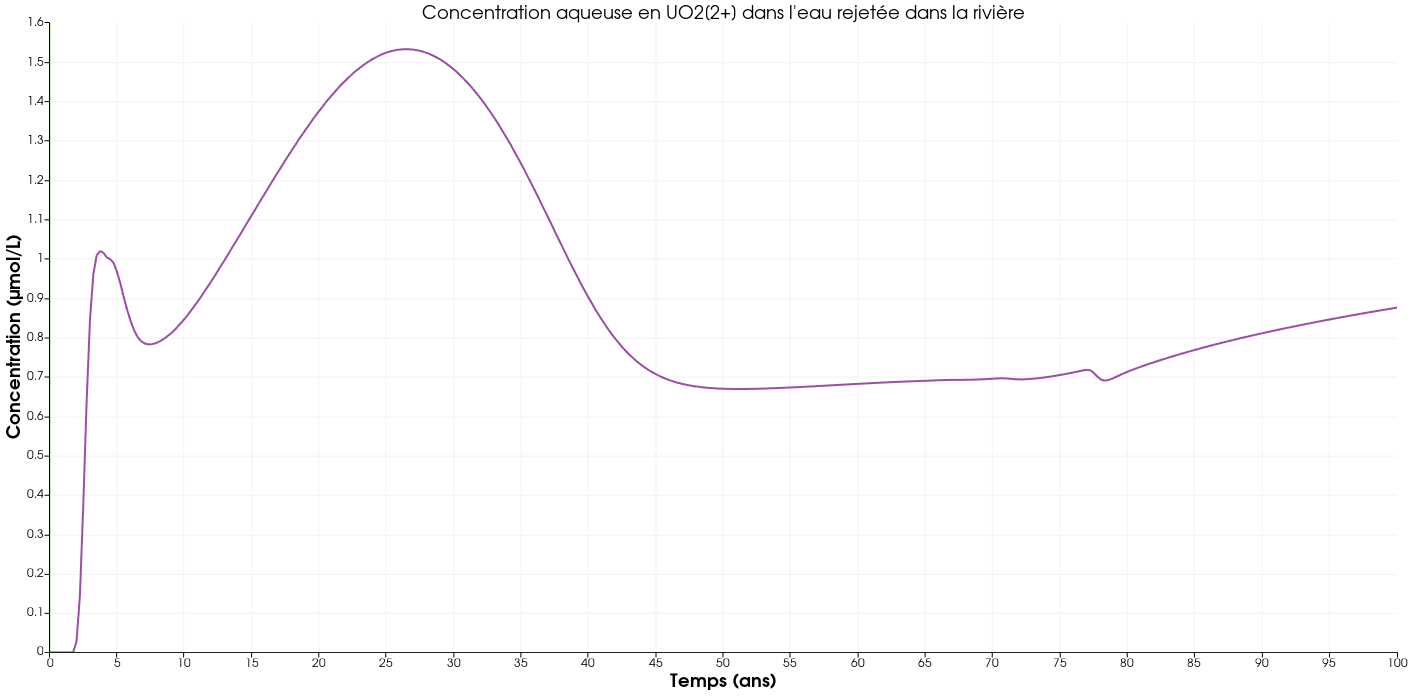
\includegraphics[width=0.9\textwidth]{III_B_2_20.png} 
        \caption{}
        \label{fig:UO2_riviere_Al}
    \end{minipage}\hfill
    \begin{minipage}{0.5\textwidth}
        \centering
        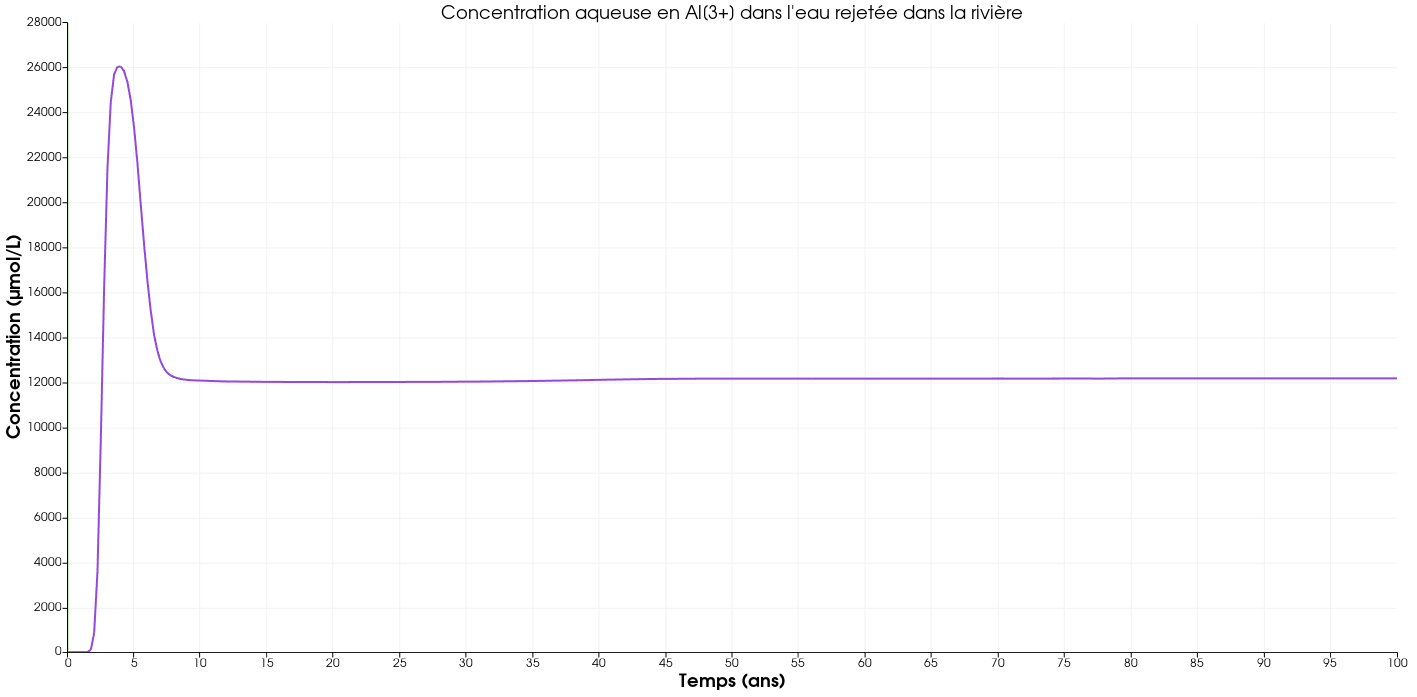
\includegraphics[width=0.9\textwidth]{III_B_2_21.png} 
        \caption{}
        \label{fig:Al_riviere_Al}
    \end{minipage}
\end{figure}


En sortie du modèle, on obtient une forte concentration en aluminium dans l’eau ($324 mg/L$ contre $200 \mu g/L$ pour la norme) et en uranium. Nous avons donc ajouté des hydroxydes d’aluminium en aval des résidus pour simuler une résine échangeuse d’ions et ajouter de la sorption.
Nous regardons alors les caractéristiques physico-chimiques de l’eau en sortie du modèle, comparée avec celle que nous avions sans $Al(OH)_3$ en aval des résidus.

(images 22, 23 et 24)

On obtient effectivement moins d’uranium en solution pendant les 50 premières années, mais ensuite, la concentration se stabilise à $0,7 \mu mol/L$ pendant 30 ans puis augmente. La sorption est alors de moins en moins efficace On remarque de plus que le pH reste acide, ce qui explique des concentrations en $UO_2^{2+}$ élevées. Pour l’aluminium, on reste bien au-delà des normes en vigueur.
Finalement, un traitement par sorption sur les hydroxydes d’aluminium semble efficace, mais pas sur le long terme. Pour envisager un tel traitement, il faut être capable de renouveler les hydroxydes d’aluminium tous les 30 ans, ou bien injecter des ions $Al^{3+}$ dans l’eau dans une station de traitement, puis réguler le pH (on n’a alors plus le problème du pH acide qui empêche l’$UO_2^{2+}$ de se fixer sur la montmorillonite). Il faut cependant faire attention aux autres polluant, notamment à l’aluminium, dont la quantité en solution est non négligeable en sortie de traitement.




\subsubsection{Modèle hydrogéologique 2D}
\paragraph{Modélisation}
Nous voulons réaliser un modèle hydrogéologique du site, afin de pouvoir analyser et prévoir à long terme l'écoulement des eaux qui traversent le site. L'eau arrive grâce aux précipitations, s'infiltre dans le site ou ruisselle, puis est évacuée en partie dans le ruisseau le Verraux en contrebas. Nous voulons donc connaître le niveau piézométrique sous le site, le profil de vitesse sur une coupe tranversale, ainsi que le débit d'exhaure au niveau du ruisseau.

La modélisation du site sera réalisée à l'aide du logiciel HYTEC, développé depuis 1993 au sein du consortium \emph{Pôle Géochimie Transport} fondé autour du Département de Géosciences de Mines ParisTech - PSL \cite{site_hytec_hydrodynamique_nodate}. 
Ce logiciel comporte un volet réalisant le calcul hydrodynamique nommé R2D2, qui est couplé avec le logiciel CHESS réalisant la simulation chimique \cite{lagneau:hal-00614306} afin d'obtenir un modèle complet de transport réactif. 

Nous réaliseront le modèle géographique du site (code n°\ref{lst:modele_topo}) à l'aide du logiciel libre GMSH \cite{gmsh_site} afin de représenter fidèlement les données de terrain. Le choix du maillage n'est pas anodin, puisqu'il va servir de support pour que la machine puisse effectuer la simulation. Par exemple, puisque la couche de surface est estimée à 4 mètres d'épaisseur, il est nécessaire que les mailles fassent moins de 4 mètres : si possible, on choisira des paramètres de maillage qui permettront d'en avoir deux ou trois dans toute cette zone. Inversement, la zone de granite sain forme un socle presque imperméable, donc les flux hydrologiques seront moins importants. C'est pourquoi un maillage plus épais pourra être choisi. Enfin, puisque la zone de résidus de traitement contient les espèces à suivre, il faut être très précis, et choisir des mailles fines pour pouvoir bien rendre compte des deux faciès.

Pour proposer un modèle convaincant du site, il est nécessaire de s’intéresser aux flux hydrogéologiques. Nous avons pour cela utilisé un rapport hydrogéologique du site, daté de 2011 \cite{societe_areva_nc_etude_2011}. Nous nous sommes basés sur les relevés des 9 piézomètres du site et avons décidé de faire une modélisation en coupe, ce qui permet à la fois de décrire « l'épaisseur » du site dans toute sa richesse tout en évitant de réaliser un modèle 3D beaucoup trop complexe. Cette coupe (figure \ref{fig:coupe_ribiere}) a été choisie car d'une part elle comprend l'intégralité de l'étendue du site (de 348 m à 395 m d'altitude), la zone de résidus et la rivière. Nous disposons également de cinq piézomètres pour nous renseigner sur le terrain.

\begin{figure}[H]
    \centering
    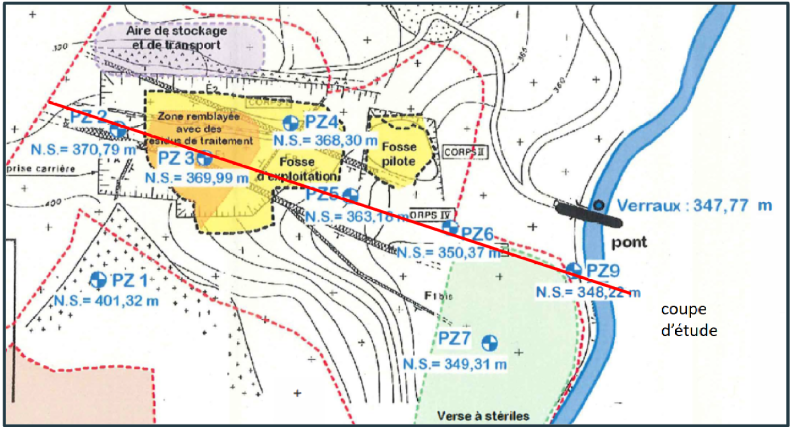
\includegraphics[width=0.8\linewidth]{III_B_3_1.png}
    \caption{Vue aérienne de la zone, avec représentation de la coupe (Google Earth)}
    \label{fig:earth_ribière}
\end{figure}


\begin{figure}[H]
    \centering
    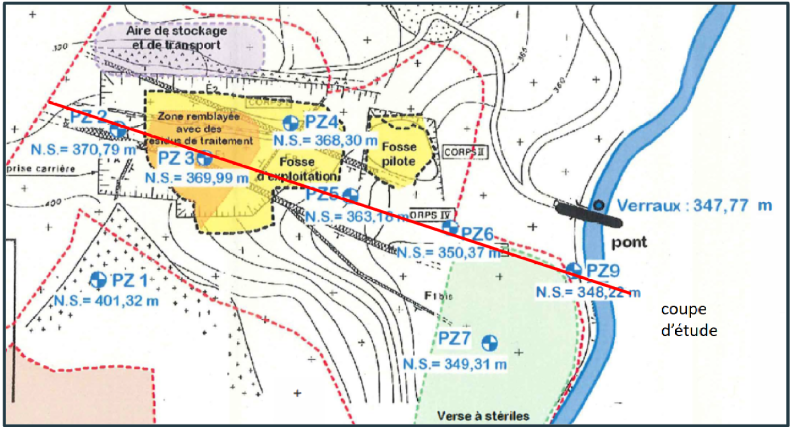
\includegraphics[width=0.8\linewidth]{III_B_3_2.png}
    \caption{Coupe réalisée pour l'étude du site (Orano) \cite{societe_areva_nc_etude_2011}}
    \label{fig:coupe_ribiere}
\end{figure}



Les relevés piézométriques permettent de définir plusieurs zones. On note tout d’abord une zone de surface, composée d’une arène granitique, et de stériles miniers au dessus de la zone de résidus, d’une épaisseur moyenne de 4 m. Celle-ci est composée de deux faciès, un faciès sableux et un faciès boueux. Une zone de granite fracturé est également présente, en dessous de laquelle on trouve une zone de granite sain. Les résidus de traitement apparaissent donc comme localisés et situés proches d’une zone de granite fracturé.

\begin{figure}[H]
    \centering
    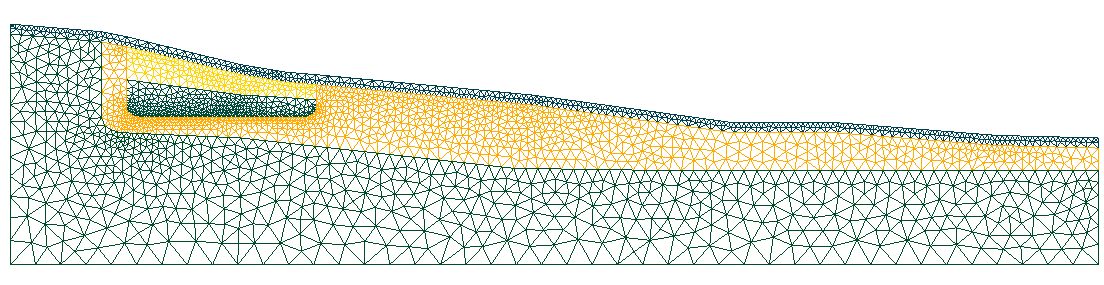
\includegraphics[width = 0.9\textwidth]{III_B_3_3.png} 
    \caption{Modélisation des différentes zones}
    \label{fig:zones_ribieres_geogebra}
\end{figure}


\begin{figure}[H]
    \centering
        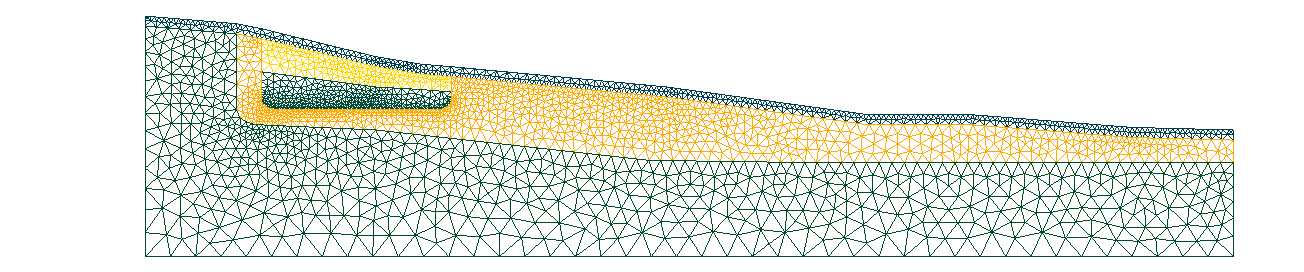
\includegraphics[width=0.9\textwidth]{III_B_3_4.png} 
        \caption{Maillage de la zone obtenu avec GMSH}
        \label{maillage_ribiere}
\end{figure}

Les relevés piézométriques permettent aussi de définir un niveau de charge: le piézomètre PZ2 indique une profondeur d’eau à environ 24 m, et le piézomètre PZ9 à 1 m, ce qui correspond au Verraux.

Les données météorologiques montrent des précipitations effectives (c’est à dire la différence entre les précipitations totales et l’évapotranspiration) variables au cours de l’année : en effet, on remarque que les mois de novembre, décembre, janvier et mars correspondent à de hautes valeurs de précipitations effectives, alors qu’elles sont presque nulles le reste de l’année. La couche de surface sert d'interface au système, et permet à l'eau en surface de pénétrer dans les autres zones, ce qui génère un flux vertical qui va notamment impacter la mobilité dans la zone de résidus. En modélisant les saisons, on modélise les fortes variations de ce flux, qui est nul une grande partie de l'année, et très intense de novembre jusqu'en janvier, ainsi qu'en mars.


\begin{figure}[H]
    \centering
    \includegraphics[width=0.8\linewidth]{III_B_3_5.png}
    \caption{Précipitations annuelles sur le site de la Ribière (Orano)}
    \label{fig:precipitations_ribiere}
\end{figure}

\paragraph{Résultats}

Les modélisations montrent l’importance de la perméabilité et de la porosité des différentes zones, puisque de faibles variations induisent des comportements différents à long terme. Il est donc nécessaire d’avoir des valeurs les plus précises possibles et les plus représentatives du site. En effet, un gradient de perméabilité trop élevé, ou bien des discontinuités de perméabilité peuvent engendrer des comportements non représentatifs, comme une remontée du traceur dans les résidus en surface. Il est également important de noter l'impact de l'anisotropie ou de l'isotropie de ces paramètres de transport. En effet, si il est possible de modéliser la perméabilité du granite sain comme isotrope, il n'en va de même pour la couche en surface. Un perméabilité verticale plus élevée qu'une perméabilité horizontale signifierait que l'eau s'infiltrant dans le sol serait plus à même de s'enfoncer dans les roches, et donc dans les couches granitiques en profondeur, que de se déplacer vers la rivière en contrebas, ce qui n'est pas cohérent. Inversement, puisque les résidus miniers sont sous forme de boue et de sable, il faut avoir une perméabilité isotrope dans ces zones.

On retrouve l'impact des paramètres de transfert dans l'étude du champ de vitesse dans la zone de précipitation. À 40 et 140 m, on remarque une infiltration plus élevée que partout ailleurs: ceci est du à une discontinuité forte de perméabilité verticale, puisque la zone de surface a une perméabilité presque dix fois plus faible que la zone de résidus selon cet axe. On remarque également sur cette simulation l'impact des saisons, avec un champ de vitesse parfois orienté vers la rivière (moment où les précipitations sont faibles) et parfois orienté verticalement (moment de fortes précipitations, donc l'infiltration prédomine). Une fois le régime permanent établie, on observe à environ 10 m du sol, un champ de vitesse toujours orienté vers la rivière: ceci correspond au déplacement de l'eau dans la couche de granite fracturé, puisque le granite sain est presque imperméable.

\begin{figure}[H]
    \centering
    \begin{minipage}{0.5\textwidth}
        \centering
        \includegraphics[width=0.9\textwidth]{III_B_3_6.png} 
        \label{fig:v_précipitations_ribiere_1}
    \end{minipage}\hfill
    \begin{minipage}{0.5\textwidth}
        \centering
        \includegraphics[width=0.9\textwidth]{III_B_3_7.png} 
        \label{fig:v_précipitations_ribiere_2}
    \end{minipage}
    \caption{Variation des vitesses d'écoulement dues aux précipitations au cours d'une année}
\end{figure}

La détermination du temps de résidence de l'eau dans le système, c'est à dire le temps qu'il faut pour que l'eau passe des résidus à la rivière, peut se faire de différentes façons. Une approximation linéaire permet un calcul d’ordre de grandeur : une modélisation par deux zones, une zone de résidus et une de granite fracturé, donne un temps de résidence d’environ 15 ans. La solution analytique donne également le même ordre de grandeur, avec un temps de résidence entre 20 et 22 ans de l'eau dans le système. Enfin, le modèle hydrogéologique montre l’évolution du traceur des résidus : on obtient ici un temps de résidence de 25 ans.

\begin{figure}[H]
    \centering
    \includegraphics[width=0.8\linewidth]{III_B_3_8.png}
    \caption{Résultat de la simulation du modèle hydrogéologique après 25 ans}
    \label{hytec_hydro_25ans}
\end{figure}

Ces résultats sont à nuancer, puisqu’à ce stade aucun modèle chimique n’a été intégré. De plus, certaines données non renseignées permettraient d’aller plus loin. Il serait possible d’affiner les bords de la fosse à résidus: nous l’avons modélisé par un trapèze, mais il est très probable que les pentes de la fosse aient une forme de gradins, afin d’assurer la stabilité de la zone. La donnée de la hauteur et de la largeur des marches permettrait une modélisation plus fine.

La nature des résidus est également peu connue. Il y a une alternance entre les deux faciès, mais la proportion réelle de chaque n’est pas renseignée. Or ces deux zones ont des comportements hydrogéologiques très différents, avec des porosité et perméabilités différentes. Une analyse géochimique des résidus pourrait donc être réalisée. De plus, seul un unique piézomètre est présent dans cette zone, ce qui induit des incertitudes : on ne dispose que des données en un point pour une zone de 80 m de long et d’environ 20m de profondeur.

Le granite fracturé aux alentours n’est pas non plus très bien connu. Des analyses seraient nécessaires pour déterminer ses caractéristiques, afin de les comparer avec celles du granite sain. Le fait que la zone soit fracturée va en effet modifier drastiquement le comportement hydrologique, puisqu’il s’agit de la zone la plus en contact avec les résidus miniers.

\paragraph{Modèle hydrogéochimique}

Une fois le modèle hydrogéologique et le modèle chimique établi, nous avons pu concevoir un nouveau modèle, prenant en compte la dynamique des flux hydrologiques et les interactions chimiques entre les éléments mis en jeu. Ceci introduit de nouvelles sensibilités, puisque l’augmentation ou la diminution de la concentration ou de la distribution d’un élément peut impacter tout le modèle. On obtient donc un modèle à la fois très sensible aux caractéristiques des roches, mais aussi à des données chimiques comme le pH.

Il a fallu néanmoins interpréter certaines données. Des relevés et analyses chimiques dans les différentes zones mises en jeu pourraient être réalisées pour évaluer précisément les compositions et concentrations en les différentes espèces. Par exemple, les taux précis en gypse ne sont pas connus partout.

\subsubsection{Conclusion pour le site}
Le modèle réalisé nous a permis de comprendre comment l’uranium pouvait circuler pour le site de la Ribière, et ce qui influence cette circulation. Ainsi, l’acidité de l’eau en entrée du système est un facteur déterminant pour la fixation de l’Uranium : en effet, si pour un pH de 6 ou de plus, l’uranium est globalement sorbé, pour un pH de 4, c’est plutôt le potassium et le magnésium qui se fixent. On obtient alors de l’uranium mobile, et donc de concentrations élevées en aval du système. De même les paramètres de transport des roches, comme la porosité et la perméabilité, vont permettre de délimiter des zones dans lesquelles l’écoulement est plus ou moins favorisé, ce qui va directement impacter la localisation et la vitesse des réactions chimiques.

Puisque l’acidité de l’eau joue un rôle si important pour ce site, il serait judicieux de contrôler le pH de l’eau de pluie, afin de pouvoir réagir et traiter si celui-ci devient trop faible. Il faudrait aussi contrôler la teneur en aluminium, puisqu’il peut y avoir précipitation de ALOH3 ce qui ferait baisser le pH. Il ne semble pas pour l’instant y avoir de problème de pollution au fer.

Le modèle construit admet toutefois certaines limites. Par exemple, nous n’avons modélisé que 9 minéraux pour les résidus. On peut se demander si ceci est bien représentatif de la zone, et il pourrait être intéressant de voir si cela reflète bien la composition réelle. En effet, l’ajout d’un seul minéral de plus peut impacter grandement les équilibres et les résultats. De même, le granite a été modélisé comme un granite usuel : peut être faudrait il étudier plus précisément le site, et notamment la zone de granite fracturé afin de voir quelles sont les particularités pour la Ribière. Enfin, on peut encore essayer d’améliorer le modèle numérique, puisque la modélisation des zones est encore un peu brutale : peut être pourrait on envisager des zones de transition, avec des modifications des paramètres physiques continues pour éviter des anomalies.

\newpage
\subsection{Atténuation de la teneur en radon gazeux}

\paragraph{} Le radon, dont la production est réalisée en grande partie dans les résidus de traitement, peut être diffusé jusqu’à la surface. Selon les caractéristiques du milieu utilisé et la profondeur des résidus, la concentration en radon à la surface est plus ou moins atténuée. Nous nous sommes inspirés du carottage réalisé dans les résidus de la Ribière (figure \ref{fig:carottage_residus}) pour construire nos modèles analytique et numérique. En effet, un modèle analytique unidimensionnel permet d’obtenir une première idée des ordres de grandeur en question, et les simulations numériques permettent d'entrer dans les détails des processus en jeu.

\subsubsection{Diffusion unidimensionnelle : modèle analytique}

\paragraph{Mise en équation et longueur caractéristique}

\paragraph{} On se place dans la couche de stériles, au-dessus de la couche de résidus, où on néglige la production de radon dans un premier temps. On prend en compte la désintégration radioactive du radon et sa diffusion, de coefficient effectif $D_{eff}=D \omega^a {S_g}^b$ ($a$ et $b$ sont les coefficients de Millington-Quirk, on peut prendre $a=b=2$ dans les stériles miniers et $a=b=1$ dans l’air ou l’eau). La concentration de radon gazeux $c(z,t)$ en mol/m$^3$ évolue selon l’équation \cite{ferry_migration_2000} :

$$
\frac{\partial \omega S_g c}{\partial t} = D_{eff}  \frac{\partial^2 c}{\partial z^2}-\lambda \omega S_g c
$$

Notons que l’on travaille dans la zone non-saturée en eau, au-dessus du niveau piézométrique. La saturation en gaz n’est donc pas uniforme dans la réalité. Ce modèle donne toutefois de bonnes estimations des ordres de grandeur en question. 

L’équation admet une longueur caractéristique de diffusion :
$$
L=\sqrt{\frac{D_{eff}}{\lambda \omega S_g }}=\sqrt{\frac{D \omega^a {S_g}^b}{\lambda \omega S_g }}
$$
Les applications numériques donnent :

\begin{figure}[H]
    \centering
    \includegraphics[width = \linewidth]{III_C_2.png}
    \caption{Longueurs caractéristiques de diffusion dans l'air, les stériles et l'eau}
    \label{fig:longueur_diffusion}
\end{figure}

Notons tout d’abord qu’une couche de protection est nécessaire : l’air ne suffit pas à atténuer le radon. On peut donc envisager d’enterrer les résidus sous une couche de stériles, ce qui leur donne une utilité et un emplacement de stockage. On remarque aussi qu’une couche d’eau peut permettre d’atténuer le radon autant qu’une couche de stérile, mais sur une épaisseur de couche 20 à 30 fois plus courte.

\newpage
\paragraph{Résolution de l'équation}

\paragraph{} On montre en annexe que le régime transitoire ne dure que quelques jours. En régime stationnaire, l’équation différentielle admet la solution :
$$
c(z)=A \exp \Big(-\frac{z}{L} \Big)+B \exp \Big( \frac{z}{L} \Big)
$$
La constante $B$ est nulle, car la concentration est nulle à l’infini. On place l’interface résidus/stériles à la cote $z=0$. L’équilibre séculaire dans les résidus implique alors l’égalité $c(0)=A=c_0$. Ainsi, on a :
$$
\left\{ \begin{array}{cl}
c(z)=c_0 \exp\Big(-\frac{z}{L}\Big) \\
a(z)=N_a \lambda c(z) =a_0 \exp\Big(-\frac{z}{L}\Big)
\end{array} \right.
$$

\paragraph{Premières conclusions sur l'épaisseur de stériles nécessaire}

\paragraph{} Dans un bâtiment habité, le niveau de référence d’activité volumique est de $a_n=300 \; \text{Bq/m}^3$. Imaginons que l’on souhaite respecter cette valeur à la surface de l’endroit où sont enfouis les résidus. Le facteur d’atténuation minimum requis est alors :
$$
r_{min}=\frac{a_0}{a_n} =3,03 \; .10^4
$$
Déterminons l’épaisseur de couche de stériles $h$ minimale nécessaire pour respecter ce facteur d’atténuation dans différentes circonstances. On a la relation :
$$
a(z)=a_0 \exp(-\frac{z}{L})
$$
Ce qui donne :
$$
h_{min}=\ln(r_{min}) \,L =10,3 \,L 
$$

Ainsi, pour atténuer le radon et respecter le niveau de référence, il est nécessaire d’ajouter une couche de protection environ dix fois plus grande que la longueur caractéristique de diffusion $L$.

\paragraph{Sensibilité des différents paramètres}
\paragraph{} Cette partie s'intéresse à la sensibilité des différents paramètres quant à leur impact sur l'efficacité de la diffusion du radon. Dans le modèle analytique, la variabilité tourne autour de la longueur caractéristique de diffusion, qui est déterminée selon le coefficient de diffusion, la porosité, la saturation et les coefficients de Millington-Quirk. Comme on s'intéresse en particulier à l'effet de la saturation en eau plus loin, focalisons nous d'abord sur les autres paramètres.

La figure \ref{fig:sens_diffusion} montre l'impact significatif que le coefficient de diffusion a sur la diffusion du radon. Sur le site de la Ribière, on peut l'estimer autour de $1 \; .10^5 \; \text{m}^2 \text{s}^{-1}$.

D'autres paramètres rentrent également en compte. La porosité et les coefficients de Millington-Quirk, qui interviennent dans l’expression du coefficient de diffusion effectif, peuvent grandement impacter la longueur effective de diffusion :
$$
L=\sqrt{\frac{D_{\text{eff}}}{\lambda \,\omega\, S_g }}=\sqrt{\frac{D \,\omega^a {S_g}^b}{\lambda\, \omega \,S_g }}
$$

Le tableau suivant donne une gamme de valeurs possibles de la longueur caractéristique $L$ en fonction de ces différents paramètres. On a retenu une saturation en gaz moyenne $S_g=0,3$.

\begin{figure}[H]
    \centering
    \includegraphics[width = \linewidth]{III_C_9.png}
    \caption{Valeur de $L$ en fonction de $a=b$, $D$ et $\omega$}
    \label{fig:sens_mq_poro}
\end{figure}

Sur le site de la Ribière, il y a une couche protectrice d'environ $6,5\;m$ au dessus des résidus. Ainsi, la longueur caractéristique doit être inférieure à $0,65\;m$ afin de respecter le niveau de référence à la surface des résidus. L'échelle de couleur donne les valeurs de $L$ pour lesquelles la référence est respectée. On peut estimer que les stériles miniers de la Ribière ont des coefficients de Millington-Quirk proches de $2$, et des porosités inférieures à $0,43$. Ainsi, le modèle analytique prévoit que le niveau de référence d'activité en radon peut être respecté.

\newpage
\subsubsection{Introduction des modèles numériques}

\paragraph{Deux modèles numériques}
\paragraph{} Nous utilisons le code de calcul HYTEC introduit plus haut dans sa dimension transport. 2 types de modèles sont utilisés par la suite pour obtenir les résultats. Les 2 modèles se limitent au cas unidimensionnel : on modélise une colonne de stériles et/ou résidus pour étudier comment le radon est produit et diffusé vers la surface. La différence entre les 2 types de modèles est la façon de modéliser le terme source de radon. Le premier type de modèle, le plus simple et le plus utilisé par la suite, ne comprend que des stériles dans la colonne. En effet pour modéliser les résidus source de radon nous utilisons une condition limite : une fugacité constante en radon à la limite stériles/résidus. Le deuxième type de modèle modélise les stériles et les résidus, la production du radon est intégré dans la roche elle-même : le gaz émane là où il y a du radium. Ce deuxième modèle n'est utilisé que dans la modélisation numérique de l'impact d'un terme source . Il s’agit là d’une présentation sommaire de ces modèles, pour des détails techniques sur leur implémentation dans le code HYTEC, se reporter à l'annexe \ref{annexe:detail_modele_radon_sec} \ref{annexe:detail_modele_radon_sub_sec}, pour les codes HYTEC utilisés se reporter aux annexes (citer annexe à ajouter)

\paragraph{Sensibilité des modèles numériques aux différents paramètres}
\paragraph{} Cette partie est consacrée à la sensibilité des paramètres sur les modèles numériques. Les simulations ont été réalisées avec un même coefficient de diffusion $D = 1.10^{-6}$ m$^2 \!$ s$^{-1}$, une porosité élevée $\omega = 0,43$ et une saturation variable dans la zone des stériles.

La figure \ref{fig:sens_hytec_mq} donne, en pourcentage, l'atténuation du radon en fonction des coefficients de Millington-Quirk sélectionnés. La simulation a été réalisée sur un modèle de 2 mètres, réduit par rapport à la réalité du site, mais cela suffit pour visualiser la sensibilité. On note que ces coefficients influent grandement sur la diffusion du radon.

Les coefficients de Van-Genuchten, notés $\alpha$ et $n$, interviennent dans l’expression de la pression capillaire, qui joue un rôle lorsque la saturation en eau n’est pas uniforme, en particulier dans un modèle vertical. En posant $S_{e,\text{eff}}$ la saturation effective en eau, son expression est donnée par :
$$
p_c (S_e)= \dfrac{1}{\alpha} \left( {S_{e,\text{eff}} }^{\frac{n}{n-1}} -1 \right)^{1/n}
$$

Les figures \ref{fig:sens_hytec_alpha} et \ref{fig:sens_hytec_n} illustrent la sensibilité des paramètres de Van-Genuchten, et montrent qu'avec des coefficients de Millington-Quirk égaux à 2, une variation d’ordre $\pm 1$ du paramètre $\alpha$ ou une variation d’ordre $\pm 0,1$ du paramètre $n$ ne modifie pas l’ordre de grandeur de la fugacité du radon à la surface.

Par la suite, nous avons fixé les paramètres de Van-Genuchten à $\alpha = 3,6$ et $n=1,56$, qui sont des valeurs moyennes pour les matériaux concernés.

\newpage
\subsubsection{Impact des précipitations}

\paragraph{Résultats analytiques}

\paragraph{} Premièrement, le modèle analytique permet d'obtenir des ordres de grandeur. Pour un coefficient de diffusion moyen $D=1,0.10^{-5} \; \text{m}^2/\text{s}$, une porosité moyenne $\omega=0,30$ et des coefficients de Millington-Quirk égaux à 2, le tableau suivant donne les longueurs caractéristiques et les épaisseurs de stériles nécessaires pour respecter le niveau de référence de $300\; \text{Bq/m}^3$, en fonction de la saturation en gaz. Plus il y d’eau dans les pores, plus la saturation en gaz est faible.

\begin{figure}[H]
    \centering
    \includegraphics[width = \linewidth]{III_C_4.png}
    \caption{Valeurs de $L$ et $h$ en fonction de la saturation en gaz}
    \label{fig:tableau_saturation}
\end{figure}

Lorsque la roche est saturée, la diffusion est moindre. Au contraire, une période sèche favorise la diffusion. Avec une épaisseur de stériles d'environ 6,5 m, le site de la Ribière peut être exposé à des activités de radon cinq à dix fois plus élevées en été quand il pleut moins souvent.

Il faut maintenant se tourner vers le modèle numérique, qui permet d’observer le régime transitoire alors que le sol est soumis aux précipitations, puis d'obtenir des courbes.

\paragraph{Résultats numériques et liens avec le modèle analytique}

\paragraph{} Nous utilisons ici le modèle numérique 2 avec des précipitations moyennes de 200 mm/an et une simulation pendant un an. La figure \ref{fig:rain_fugacity} donne la fugacité du radon en fonction de la cote (où l'origine est au niveau des résidus), en échelle logarithmique. La courbe bleue correspond au cas pluvieux et la courbe brune au cas témoin.

L’échelle logarithmique montre que la concentration en radon est divisée par un facteur 10, ce qui était dans l'ordre de grandeur donné par le modèle analytique. On en déduit que les précipitations sont bénéfiques quant à l’atténuation du radon gazeux. Le phénomène en jeu est la dissolution du radon dans l’eau. La présence d’eau augmente la pression, donc déplace l’équilibre de Henry entre le radon gazeux et le radon aqueux, dont la concentration augmente dans la zone humide.

\newpage
\subsubsection{Impact d'un terme source au sein des stériles}

\paragraph{} Sur la plupart des anciens sites miniers, les résidus de traitement sont recouverts de stériles miniers. Ces derniers ont des activités plus faibles en uranium et en radium, et donc produisent moins de radon. Néanmoins, il est important de quantifier l'impact d'une source de radon au sein des stériles pour s'assurer que la décision de les utiliser pour recouvrir les résidus est sans danger.

\paragraph{Résultats du modèle analytique}

\paragraph{} Le modèle analytique, avec l'ajout d'un terme source dans les stéril de radon dans les stériles est négligeable. Sinon, la production de radon dans les stériles peut être importante. Dans tous les cas, au bout d'une certaine altitude, seule la production de radon dans les stériles n'est visible.

Ainsi, mettre une très grande couche de stériles permet d'atténuer complètement l'émanation de radon des résidus, mais cela n'a de sens que si les stériles eux-mêmes ne génèrent pas une grande quantité de radon. En effet, il se peut que le radon détecté à la surface soit issu des stériles, et non pas des résidus.

Donnons un ordre de grandeur du coefficient $R$ sur le site de la Ribière. On prend les valeurs :
\begin{itemize}
  \item Stériles non saturés $E=0,01$ ; résidus saturés $E_r=0,3$ 
  \item Stériles miniers $\omega = 0,34$ ; résidus $\omega_r = 0,43 $
  \item Stériles miniers et résidus : $\rho \simeq \rho_r$
  \item Stériles non saturés $S_g = 0,67$; résidus saturés $S_{g,r}=0,03$
  \item Stériles miniers $A_{Ra,s}= 0 - 0,04 - 0,4 \; \text{Bq/g}$, résidus $A_{Ra,s}= 4,0 \; \text{Bq/g}$
\end{itemize}
On obtient $ R=7,0\%$, ce qui signifie que la production de radon dans les stériles, même le radium y est environ trois fois moins actif, a une influence sur la courbe de diffusion du radon. On peut ainsi comparer les concentrations à la surface, avec ou sans terme source ($L=0,6$ m, $h=6,5$ m) :
\begin{itemize}
  \item Pour $A_{Ra,s}=0$ Bq/g : $c(h) = 1,4 \; .10^{-16} \text{mol/m}^3$ soit 180 Bq/m$^3$
  \item Pour $A_{Ra,s}=0,04$ Bq/g : $c(h) = 3,0 \; .10^{-16} \text{mol/m}^3$ soit 373 Bq/m$^3$
  \item Pour $A_{Ra,s}=0,4$ Bq/g : $c(h) = 1,7 \; .10^{-15} \text{mol/m}^3$ soit $2,1 \; .10^3$ Bq/m$^3$
\end{itemize}

Ainsi, avec une activité de radium cent fois plus faible dans les stériles, l'activité du radon à la surface est multipliée par deux, et avec une activité de radium seulement dix fois plus faible, l'activité du radon est multipliée par un facteur 10 à la surface.

Cette étude analytique permet donc de penser que les stériles doivent également être surveillés en terme de teneur en radium, car ils peuvent amplement modifier la teneur en radon gazeux à la surface.

\paragraph{Résultats du modèle numérique}
\paragraph{} Le modèle numérique utilisé est du deuxième type : modélisation de l'émanation du radon dans toute la colonne sans condition aux limites. Dans le cas de ce modèle, nous sommes limités par la précision des calculs internes de HYTEC, ainsi nous ne pouvons pas travailler avec les fugacités en radon réellement présentes sur le site de la Ribière. On va donc s'intéresser à des fugacités relatives par rapport à une

\subsubsection{Conclusions sur le risque radon}

\newpage
\section{Synthèse des enjeux}
\subsection{Aspect socio-économique du traitement de l’eau}
\subsection{Ouverture à l’international}

\newpage
\section*{Conclusion}
\addcontentsline{toc}{section}{Conclusion}

\newpage
\section*{Références bibliographiques}
\addcontentsline{toc}{section}{Références bibliographiques}

\printbibliography[heading=none] % j'ai trouvé !!!
%Bien joué ! J'ai déplacé avant les annexes car je crois que cette bibliographie n'est pas une annexe car on a utilisé les refs dans le rapport --S

%%%%%% ANNEXES %%%%%%%
\newpage
\appendix
\pagenumbering{roman}
\titleformat{\section}
    {\Large\bfseries}
    {Annexe \thesection \: -}
    {0.5 em}
    {}

\newpage
\section{Figures utiles}

\begin{figure}[H]
    \centering
    \includegraphics[width=13cm]{II_A2_1.png}
    \caption{Chaîne de désintégration de l’uranium}
    \label{fig:desintegration_uranium}
\end{figure}

\begin{figure}[H]
    \centering
    \includegraphics[width=10cm]{II_A2_4.png}
    \caption{Exposition moyenne de la population aux rayonnements ionisants}
    \label{fig:exposition_moyenne}
\end{figure}

\begin{figure}[H]
    \centering
    \includegraphics[width=8cm]{II_A2_5.png}
    \caption{Comparaison des normes radiologiques sur le radon}
    \label{fig:comparaison_normes}
\end{figure}

\begin{figure}[H]
    \centering
    \includegraphics[width = 14.5cm]{III_C_1.png}
    \caption{Carottage dans les résidus du site de la Ribière}
    \label{fig:carottage_residus}
\end{figure}

\begin{figure}[H]
    \centering
    \includegraphics[height = 0.4 \textheight]{III_C_8.png}
    \caption{Fonction $\exp(-z/L)$ en fonction du coefficient de diffusion}
    \label{fig:sens_diffusion}
\end{figure}

\begin{figure}[H]
    \centering
    \includegraphics[height = 0.4 \textheight]{III_C_10.png}
    \caption{Résultats HYTEC en fonction des coefficients de Millington-Quirk}
    \label{fig:sens_hytec_mq}
\end{figure}


% \begin{figure}[H]
%     \centering
%     \makebox[\textwidth]{\makebox[1.3\textwidth]{\begin{minipage}{0.6\textwidth}
%         \centering
%         \includegraphics[height = 0.3 \textheight]{III_C_11.png}
%         \caption{Résultats HYTEC en fonction de $\alpha$, à $n=1,56$ fixé}
%         \label{fig:sens_hytec_alpha}
%     \end{minipage}\hfill
%     \begin{minipage}{0.6\textwidth}
%         \centering
%         \includegraphics[height = 0.3 \textheight]{III_C_12.png}
%         \caption{Résultats HYTEC en fonction de $n$, à $\alpha=3,6$ fixé}
%       \label{fig:sens_hytec_n}
%     \end{minipage}}}
% \end{figure}


\begin{figure}[H]
    \centering
    \includegraphics[height = 0.26 \textheight]{III_C_11.png}
    \caption{Résultats HYTEC en fonction de $\alpha$, à $n=1,56$ fixé}
    \label{fig:sens_hytec_alpha}
\end{figure}
\begin{figure}[H]
    \centering
    \includegraphics[height = 0.26 \textheight]{III_C_12.png}
    \caption{Résultats HYTEC en fonction de $n$, à $\alpha=3,6$ fixé}
    \label{fig:sens_hytec_n}
\end{figure}
\begin{figure}[H]
    \centering
    \includegraphics[height = 0.25 \textheight]{III_C_6.png}
    \caption{Fugacité du radon avec ou sans précipitations}
    \label{fig:rain_fugacity}
\end{figure}

\newpage
\section{Hydrogéologie : la loi de Darcy}
\subsection{La loi de Darcy}

\paragraph{} Les roches sont poreuses : elles peuvent stocker de l’eau. On appelle porosité le rapport $p=\dfrac{V_{libre}}{V_{tot}}$, où $V_{tot}$ représentant le volume total de l'échantillon dont on veut mesurer la porosité, et $V_{libre}$ le volume qui y est laissé inoccupé. Ce rapport traduit la capacité de stockage d'une roche et peut atteindre jusqu’à 60\% pour les argiles, ou valoir quelques dixièmes de pourcents pour certains granites. Cela explique que les roches laissent circuler l’eau. Cependant, la porosité de définit pas la facilité avec laquelle l’eau peut circuler dans les roches. Cette propriété, liée à la porosité mais non déductible de cette dernière, s’appelle la perméabilité.

L’hydrogéologie est l’étude de l’écoulement de l’eau dans les roches. Un premier modèle permettant d’étudier le phénomène est la loi de Darcy, du nom de l’hydraulicien Henry Darcy qui l’a établie. Elle s’écrit : $V = - K\cdot \nabla(h)$ où V est la vitesse de Darcy, K la perméabilité et h la charge. %et c'est nabla pas grad 

Le logiciel HYTEC utilisé pour le calcul du modèle hydrogéologique détermine les écoulements de l’eau dans les roches par des calculs de charge en tenant compte des conditions imposées aux limites en charge, des perméabilités des milieux traversés et de la loi de Darcy. Le modèle du site de la Ribière étant constitué d’un ensemble de zones de perméabilité uniforme, nous établissons dans un premier temps le profil de charge dans des cas très simples de modèles à une dimension, et étudions rapidement un modèle très simple de prise en compte des précipitations. La vitesse de Darcy représente alors le débit de l’écoulement à travers la roche ou son opposé selon l'orientation du problème, le débit étant pris positif. 
\subsection{Modèles simples pour la compréhension des phénomènes}
\subsubsection{Variations de perméabilité}
\paragraph{} On considère une zone d’épaisseur L et de perméabilité uniforme K (figure \ref{fig:ecoulement_permea_uniforme}).

\begin{figure}[H]
    \centering
    \includegraphics[width=6cm]{A_III_B_1.png}
    \caption{Ecoulement dans une roche de perméabilité uniforme}
    \label{fig:ecoulement_permea_uniforme}
\end{figure}
%super ! ouais ça rend pas mal du tou je trouve mdr bravo à toi en ft cest bcp trop penible overleaf
De l’eau s’y écoule avec un débit Q. On se place au régime stationnaire. La charge en amont de la roche est notée $h_1$ et la charge en aval est notée $h_2$.

La loi de Darcy relie les paramètres du problème :

$$ Q = -V = K\nabla(h) = K\,\frac{dh}{dx} $$


La conservation de la masse impose un débit constant dans toute l’épaisseur de la roche. Le gradient de charge est donc constant et  $Q = K\dfrac{\Delta h}{L} $.

On considère à présent une deux zones de roches superposées d’épaisseurs respectives $L_1$ et $L_2$ et de perméabilités respectives $K_1$ et $K_2$ (figure \ref{fig:ecoulement_permea_variable}).

\begin{figure}[H]
    \centering
    \includegraphics[width=6cm]{A_III_B_2.png}
    \caption{Ecoulement dans une roche de perméabilité variable}
    \label{fig:ecoulement_permea_variable}
\end{figure}

On cherche à déterminer, au régime stationnaire, le profil de charge. Pour ce faire, on se place au régime stationnaire et on fixe les valeurs $h_2$ et $h_0$ en amont et en aval du système. La conservation de la masse empêche l’accumulation d’eau dans une tranche élémentaire de roche : le débit est donc uniforme sur tout le système. On note $h_1$ la valeur de la charge à l’interface entre les roches.

Grâce à la loi de Darcy,  l’égalité du débit s’écrit alors : 

$$ K_1 \,\frac{h_2 - h_1}{L_1} = K_2\, \frac{h_1 - h_0}{L_2} $$

D’où l’on tire :

$$ \left(\frac{K_1}{L_1} + \frac{K_2}{L_2}\right)\cdot h_1 = \frac{K_2}{L_2} \,h_0 + \frac{K_1}{L_1}\, h_2$$

On peut alors exprimer Q en fonction de $h_0$ et $h_2$ :

\begin{equation}
\begin{split}
Q &= \dfrac{K_1}{L_1} \left(h_0 - \dfrac{K_1}{L_1(\frac{K_1}{L_1} + \frac{K_2}{L_2})}\,h_2 - \dfrac{K_2}{L_2(\frac{K_1}{L_1} + \frac{K_2}{L_2})}\,h_0\right)\\
&\\
& = \dfrac{K_1}{L_1}\left(h_2\,\left(1 -  \dfrac{K_1}{L_1\,(\frac{K_1}{L_1} + \frac{K_2}{L_2})}\right) - h_0\dfrac{K_2}{L_2\,(\frac{K_1}{L_1} + \frac{K_2}{L_2})}\right)\\ 
&\\
& = \dfrac{K_1}{L_1}\left(h_2\,\dfrac{\frac{K_2}{L_2}}{\frac{K_1}{L_1} + \frac{K_2}{L_2}} - h_0\,\dfrac{\frac{K_2}{L_2}}{\frac{K_1}{L_1} + \frac{K_2}{L_2}}\right)\\
&\\
& = \dfrac{\dfrac{K_1K_2}{L_1L_2}}{\dfrac{K_1}{L_1} + \dfrac{K_2}{L_2}}\,(h_2 - h_0)
\end{split}
\end{equation}


On peut alors définir une perméabilité équivalente pour le système complet, en considérant que sa longueur équivalente est $L_{eq} = L_1 + L_2$ :

$$ Q = \frac{K_{eq}}{L_{eq}}\,(h_0 - h_2) $$

Il vient :

$$ K_{eq} = (L_1 + L_2)\,\dfrac{\dfrac{K_1K_2}{L_1L_2}}{\dfrac{K_1}{L_1} + \dfrac{K_2}{L_2}} $$

On peut généraliser la relation à un nombre quelconque de perméabilités en série en notant que le rapport $ \dfrac{L}{K} $ est additif :  

$$ \dfrac{L_{eq}}{K_{eq}} = \dfrac{L_1}{K_1} + \dfrac{L_2}{K_2} $$

Pour n zones de roches en série de perméabilités et longueurs respectives $K_{i}$ et $L_{i}$, la perméabilité équivalente est :
$$K_{eq} = \frac{\sum\limits_{i=1}^{n}L_i}{\sum\limits_{i=1}^{n}\frac{K_i}{L_i}} $$

On est alors en mesure, connaissant les conditions aux bords d’un système de perméabilités en série, de déterminer la charge aux interfaces entre deux zones de roches en se ramenant à un problème à deux perméabilités par un calcul de perméabilité équivalente. Alors, le débit et la perméabilité étant constants dans une même zone rocheuse, la loi de Darcy permet d’affirmer que le gradient de charge y est aussi constant. On peut alors calculer la charge en tout point du système.

Le système s’apparente alors à un système électrostatique, et on peut dresser l’analogie suivante :

\begin{center}
\begin{tabular}{ |c |c |}
\hline
 \textbf{Hydrologie} & \textbf{Électrocinétique} \\ 
 \hline
 Charge $h$ & Potentiel $V$ \\ 
 \hline
 Vitesse de Darcy $v$ & Densité de courant $j$  \\
 \hline
Perméabilité $K$ & Conductance électrique $\gamma$  \\
 \hline
Loi de Darcy : $v = -K\,\nabla h$ & $j = -\gamma\,\nabla V$  \\
 \hline
\end{tabular}
\end{center}

\subsection{Une première intégration des précipitations au modèle}
\paragraph{} On considère le problème unidimensionnel suivant : une roche de perméabilité $K$ et de longueur $L$ est traversée par un écoulement stationnaire.

\begin{figure}[H]
    \centering
    \includegraphics[width=13cm]{A_III_B_3.png}
    \caption{Écoulement selon la direction x dans une roche de perméabilité uniforme soumise à des précipitations}
    \label{fig:ecoulement_précipitations}
\end{figure}
\newpage
Pour modéliser des précipitations (plus précisément leur infiltration dans les roches), on ajoute de l’eau de manière uniforme sur toute la longueur de la roche. On note q l’apport d’eau en $\text{m}^3/\text{s}/\text{m}$

\begin{figure}[H]
    \centering
    \includegraphics[width=6cm]{A_III_B_4.png}
    \caption{à légender}
    \label{fig:schema_carre_ecoulement}%on touche pas au label
\end{figure}


On écrit l’équation de conservation de la charge d'après la figure \ref{fig:schema_carre_ecoulement} :
$$ \text{div} (Q)=q$$

On a donc $\dfrac{\text{d}Q}{\text{d}x}=q$.
Or $Q= -K\, \dfrac{dh}{dx}$.

On obtient donc l’équation différentielle du second ordre $\dfrac{\text{d}^2h}{\text{d}x^2}=-q/K$. 
Pour la résoudre entièrement, il est nécessaire de connaître les conditions aux limites. 

En supposant les conditions en charge en $x = 0$ et $x = L$ connues, on obtient le profil de charge dans le roche :

$$h(x) = -\frac{Q}{2K}x^2 + \left(\frac{h_2 - h_1}{L} + \frac{QL}{2K}\right)x + h_2$$


En supposant la condition en charge en $x = L$ et le débit entrant $Q_0 = K \dfrac{\text{d}h}{\text{d}x}(x = 0)$ connus, on obtient le profil de charges dans la roche :
$$h(x) = -\frac{Q}{2K}x^2 + \frac{Q_0}x + h_2$$

\newpage
\section{Radon : détails des raisonnements}
\label{annexe:detail_modele_radon_sec}
\subsection{Estimation du facteur d'émanation}
\label{annexe:emanation}

\paragraph{} La formule suivante du facteur d'émanation $F_e$ est donnée en fonction du paramètre $x=2\,R_s/D$ et on a tracé la fonction selon le diamètre, avec $R_s=30$ nm dans le grain (figure \ref{fig:facteur_emanation}).

$$
F_e (x)= \frac{3}{4} \,x\,(1- \frac{x^2}{12} )
$$

\begin{figure}[H]
    \centering
    \includegraphics[width=10cm]{II_A2_2.png}
    \caption{Facteur d’émanation en fonction du diamètre des grains}
    \label{fig:facteur_emanation}
\end{figure}

\subsection{Équilibre séculaire : calculs }
\label{annexe:seculaire}

\paragraph{} Le but est de déterminer l'activité volumique du radon au sein des résidus, de concentration en radium solide $c_{Ra}$ constante (mol/m$^3$). 

La proportion de quantité de matière de $Rn(g)$ créée par désintégration atteignant les porosités par unité de volume est $E c_{Ra}$, où $E$ est le facteur d’émanation. On note $\lambda_{Ra}$ et $\lambda_{Rn}$ les coefficients de désintégration du radium et du radon en $s^{-1}$. 

On caractérise le milieu par une masse volumique $\rho$, une porosité $\omega$ et une saturation en gaz $S_g$. La concentration en radon $c_{Rn}$ en mol/m$^3$ évolue selon l'équation :

$$
\frac{\text{d} \omega S_g c_{Rn}}{\text{d}t} = - \lambda_{Rn}\cdot \omega\cdot S_g \cdot c_{Rn} + \lambda_{Ra} \cdot E \cdot(1-\omega)\cdot c_{Ra}
$$

A l'équilibre séculaire, $c_{Rn}(t)=c_0$ et ainsi :

$$
c_0 = \frac{ \lambda_{Ra} E (1-\omega) c_{Ra} }{\lambda_{Rn} \omega S_g}
$$

On notera les activités en radon et en radium dans les résidus, avec $N_a$ le nombre d'Avogadro :
\begin{itemize}
  \item $a_{Rn}= \lambda_{Rn} N_a c_{Rn}$ en Bq/m$^3$
  \item $A_{Ra}= \dfrac{\lambda_{Ra} N_a }{\rho} c_{Ra}$ en Bq/kg
\end{itemize}

Ce qui permet d'obtenir les expressions, et les applications numériques dans le cas du site de la Ribière, avec $\rho = 2,6 \;.10^3 \text{ kg/m}^3$, $\omega= 0,43$, $S_g=0,3$ et $A_{Ra}=4 000$ Bq/kg :

$$
c_0 = \dfrac{ E \,(1-\omega)\, \rho }{\lambda_{Rn}\: \omega \,S_g N_a} A_{Ra} = 7,1.10^{-12} \text{ mol/m}^3
$$
$$
a_0=\lambda_{Rn} N_a c_0 =\frac{E(1-\omega)\rho}{\omega S_g} A_{Ra} =9,1 \, \text{MBq/m}^3
$$

\subsection{Dose efficace : estimation du facteur $r$}
\label{annexe:estimation_r}

\paragraph{} On cherche à retrouver la valeur $r=7,8 \; .10^{-6} \;\text{m}\text{Sv}/(\text{Bq}/\text{m}^3.\text{h})$.

L’IRSN donne un lien \cite{irsn_ineris_radon_nodate} entre l’activité volumique du radon $a$ et l’énergie alpha potentielle volumique $e_{\alpha}$ (l’énergie libérée par les désintégrations successives par unité de volume) à l’aide du facteur d’équilibre $F$ et du coefficient de conversion $f=5,56$ nJ/Bq :
$$
F=\frac{e_{\alpha}}{f\cdot a}
$$

On sait que le risque radiologique du radon gazeux se situe au niveau des poumons. Le volume d’air inspiré par une personne est égal à $V=4,8.10^3 \;  \text{m}^3/\text{an}=0,55 \; \text{m}^3/\text{h} $. Or, la dose absorbée en Grey pendant une durée $\Delta t$ et avec des poumons moyens de masse $m=1,2$ kg est donnée par : 
$$
d_{Gy}=\frac{E_{\text{absorbée}}}{m}=\frac{e_{\alpha} V \Delta t}{m}=\frac{F\,f\,V\Delta t}{m}\,a
$$
On peut en déduire la dose efficace en Sieverts, qui est pondérée par un facteur $\omega_{rad}=20$ (radioactivité alpha) et un facteur $\omega_{tissu}=0,12$ (tissus pulmonaires) :
$$
d_{Sv}=\omega_{rad}\: \omega_{tissu} \: d_{Gy} = r'\cdot F\cdot\Delta t\cdot a
$$
On a alors posé le facteur $r'$ :
$$
r'= \frac{\omega_{rad}\, \omega_{tissu}\,  f\,V}{m}=6,1.10^{-6} \; \text{m}\text{Sv}/(\text{Bq}/\text{m}^3.\text{h})
$$
Qui constitue un ordre de grandeur raisonnable du facteur r, avec un écart relatif de 22$\%$.

\subsection{Diffusion unidimensionnelle : régime transitoire}

Notons $\text{erfc}$ la fonction d’erreur complémentaire :
$$
\text{erfc}(u)=\frac{2}{\sqrt{\pi}} \int_{u}^{+\infty } e^{-\xi^2} \text{d}\xi
$$
Il existe une solution de l’équation en régime transitoire avec $c(0,t)=c_0$, de la forme :
$$
c(z,t)=\frac{c_0}{2} \left( \exp\!\left(-\frac{z}{L}\right) \, \text{erfc}\!\left(\frac{z}{2L\sqrt{ \lambda t}} - \sqrt{\lambda t}\right) + \exp\!\left(\frac{z}{L}\right) \, \text{erfc}\!\left(\frac{z}{2L\sqrt{\lambda t}} + \sqrt{\lambda t} \right) \right)
$$
L’expression admet un temps caractéristique de convergence vers l’état stationnaire :
$$
\tau=\frac{1}{\lambda}=4,8 \; .10^5 \; \text{s}=5\text{j} \; 13\text{h}
$$
Les graphiques suivants illustrent la progression de la solution transitoire vers l'état stationnaire, de gauche à droite.
\begin{figure}[H]
    \centering
    \includegraphics[width = \linewidth]{III_C_3.png}
    \caption{Transition vers l'état stationnaire}
    \label{fig:diffusion_transitoire}
\end{figure}

Ainsi, au bout d'une ou deux semaines, le régime stationnaire est atteint.

\subsection{Détails des modèles HYTEC utilisés}
\label{annexe:detail_modele_radon_sub_sec}
\paragraph{}Cette partie explicite des détails propres aux implémentations dans HYTEC des différents modèles utilisés

\paragraph{Deux codes HYTEC}l'étude du transport vers la surface du gaz radon, la prise en compte de sa désintégration radioactive est primordiale, en effet sa demie-vie de 2,8 jours est assez courte pour qu'une part non négligeable du gaz se soit désintégrée  avant d'arriver à la surface : ce phénomène va avoir un impact sur sa diffusion. Cette décroissance radioactive n'est pas prise en compte par HYTEC par défaut, nous avons donc utilisé 2 méthodes pour pallier à ce problème.
% SECTION MAL ECRITE A REVOIR
La première consiste à utiliser les outils que le code HYTEC nous met à sa disposition et de "détourner" leurs usages. Dans notre cas, nous créons un minéral fictif composé uniquement de radon ; le code permet définir les paramètres de l'équation de création du minéral: 
$$Rn_{aq} \quad \text{ou} \quad Rn_{g} \rightarrow Rn_{mineral}$$
On définit cette réaction par sa cinétique : 
$$ \frac{d\left[ Rn_{mineral} \right]}{dt}=\lambda_{Rn} \left[ Rn_{aq \quad ou \quad g} \right] $$

Nous introduisons par la suite ce minéral en quantité nulle dans toutes les zones de la simulation, ainsi la décomposition du radon est modélisée par sa précipitation sous la forme de ce minéral fictif qui ne réagit avec rien et reste sur place.

La deuxième méthode consiste à modifier le code HYTEC lui même en incorporant cette décroissance directement dans l'équation de transport du Radon dans le code source. Cette modification a été mise en place par Irina Sin, le "nouveau" code HYTEC est formellement renommé HYTEC\_R.

dans la suite l'une et l'autre méthode sont utilisés selon l'accès ou non (au temps de la simulation) au code HYTEC\_R, ou encore des éventuels problèmes de compatibilité du code HYTEC\_R avec le modèle utilisé. Cela n'a pas d'impact sur les résultats car les 2 méthodes sont équivalentes.
\paragraph{Modèles de type "condition aux limites" } Le permier type de modèle utilisé est le plus simple : on modélise une colonne verticale stériles avec éventuellement une zone d'air au dessus selon les besoins. On ne modélise pas ici les résidus à proprement parler, on modélise juste leur impact sur les stériles. Cet impact se traduit par une fugacitée constante en radon à la limite basse de la zone stériles du modèle (limite qui est en réalité l'interface stériles/résidus). HYTEC a besoin d'un condition limite en fugacité (pression partielle en radon dans le gaz contenu dans les pores), on ne connaît pas cette valeur : on en propose un calcul dans la partie \ref{annexe:fug_act} ci-dessous.

\paragraph{Modèles de type "production de radon dans toute la colonne"}Ce deuxième type de modèle met en place, pour modéliser la création de radon dans toute la colonne, un


\subsection{Relation entre fugacité et activité du radon}
\label{annexe:fug_act}
\paragraph{}Les modèles numériques demandent, pour les gaz, des conditions initiales exprimées en fugacité. Le but de cette partie est de formaliser les relations reliant l’activité du radon gazeux $a(z,t)$ en Bq/m$^3$, la concentration en radon gazeux $c(z,t)$ en mol/m$^3$ et la fugacité du radon gazeux $P_{Rn} (z,t)$ en Pa. La relation des gaz parfaits donne, à une température $T$ et avec $R$ la constante des gaz parfaits :
$$
P_{Rn} (z,t)=\frac{n_{Rn} RT}{V}=RT\,c(z,t)=\frac{RT}{N_a \lambda}\, a(z,t)
$$

On en déduit, pour une activité du radon $a_0=9,1 \; MBq/m^3$ dans les résidus, la fugacité initiale $p_0=p(0,t)$ à entrer dans le modèle HYTEC :
$$
p_0=1,7 .10^{-8} \; \text{Pa}=1,7 .10^{-13} \; \text{bar}
$$

\subsection{Impact d'un terme source dans les stériles}
\label{annexe:termesource}

Les stériles contiennent du radium d’activité massique $A_{Ra,s}$. Le radium se désintègre avec un coefficient $\lambda_{Ra}$. Ajoutons un terme source dans l’équation différentielle en concentration de radon $c(z,t)$ (exprimée en mol/m$^3$) :
$$
\frac{\partial \omega S_g c}{\partial t} = D_{eff}  \frac{\partial^2 c}{\partial z^2}-\lambda \omega S_g c + \lambda_{Ra}(1-\omega)E c_{Ra}
$$
Cette équation se résout également en régime stationnaire, pour $c=c(z)$ et $L=\sqrt{\frac{D_{eff}}{\lambda \omega S_g }}$ :
$$
\frac{\text{d}^2 c}{\text{d}z^2} - \frac{c}{L^2}= \frac{\lambda_{Ra}(1-\omega)E}{D_{eff}} c_{Ra}
$$
On obtient, avec les mêmes conditions aux limites :
$$
c(z)= c_s + (c_0 - c_s) \exp(-z/L)
$$
On a posé la concentration source $c_s$ :
$$
c_s = \frac{(1-\omega)E\rho_s}{\lambda_{Rn}\omega S_g N_a} A_{Ra,s} 
$$
Ce résultat est à comparer avec la solution sans terme source, de la forme $c_0 \exp(-z/L)$. On calcule donc le rapport suivant :
$$
R=\dfrac{c_s}{c_0}= \dfrac{\dfrac{(1-\omega)E\rho}{\lambda_{Rn}\omega S_g N_a} A_{Ra,s}}{\dfrac{ E_r (1-\omega_r) \rho_r }{\lambda_{Rn} \omega_r S_{g,r} N_a} A_{Ra,r}} = \frac{E}{E_r} \frac{(1-1/\omega)}{(1-1/\omega_r)} \frac{\rho}{\rho_r} \frac{S_{g,r}}{S_g} \frac{A_{Ra,s}}{A_{Ra,r}}
$$
On a alors :
$$
c(z)=c_s + c_0(1-R) \exp(-z/L)
$$
L'interprétation de cette expression est claire :
\begin{itemize}
  \item Si $R\ll 1$, alors la production de radon dans les stériles est négligeable.
  \item Sinon, la production de radon dans les stériles peut être importante.
  \item Dans tous les cas, au bout d'une certaine altitude, seule la production de radon dans les stériles n'est visible.
\end{itemize}

\renewcommand\lstlistingname{Code n°}
\renewcommand\lstlistlistingname{}
\newpage
\section{Liste des codes utilisés}
\lstlistoflistings
\newpage
\section{Code HYTEC Utilisé }
\label{lst:modele_hydro_chimie_final}
\lstinputlisting[language=hytec, caption = Modèle couplé hydrogéologique et chimique]{modele-final-100ans.htc}
\newpage
\lstinputlisting[language=hytec, caption = Modèle géochimique (sans injection d'aluminium) ]{ribieresable.htc}
\newpage
\lstinputlisting[language=hytec, caption = Modèle géochimique (avec injection d'aluminium) ]{ribieresablealumax.htc}


\newpage
\section{Modèle topographique du site}
\lstinputlisting[language=gmsh,caption = Modèle topographique du site de La Ribière ]{ribiere.geo}
\label{lst:modele_topo}

\newpage
\lstinputlisting[language=hytec, caption=Radon : modèle vertical à deux zones]{radon_sol_air.htc}

\newpage
\lstinputlisting[language=hytec, caption=Radon : modèle vertical avec précipitations]{radon_pluie.htc}

\newpage
\section{Résultats des simulations numériques HYTEC}


\newpage
\listoffigures


\end{document}
